\documentclass[a4paper,landscape,10pt]{article}
\usepackage[margin=10mm]{geometry}
\usepackage[T1]{fontenc}
\usepackage{lmodern}
\usepackage{helvet}
\renewcommand{\familydefault}{\sfdefault}
\usepackage{tikz}
\usetikzlibrary{arrows.meta}
\usepackage{xcolor}
\usepackage{booktabs}
\pagestyle{empty}
\setlength{\parindent}{0pt}
\definecolor{ft0}{HTML}{CFE4F2}
\definecolor{ft1}{HTML}{FBE2B4}
\definecolor{ft2}{HTML}{D4E9CC}
\definecolor{ft3}{HTML}{E5D3EA}
\definecolor{ft4}{HTML}{F5CACA}
\begin{document}

{\LARGE\bfseries Bilderwand -- layout candidates}\\[4pt]
{\small Target 180x120 cm $\pm$ 10.0 cm, nominal gap free in
[1.5, 6.0] cm, orientation fixed, sizes are measured outer dimensions.
Max.\ gap deviation = largest difference between an actual gap and the layout's nominal gap;
notches = parts of the outer border not covered by a frame or a regular gap. Ranked by a combined
score (gap uniformity first, border sharpness second, then number of frames).}\\[10pt]
\begin{minipage}[t]{0.6\textwidth}\vspace{0pt}
\begin{tabular}{@{}r l r r r r l c@{}}
\toprule
\# & size (cm) & gap & frames & max dev & mean dev & notches & corners \\
\midrule
1 & 172.5 $\times$ 115.5 & 2.5 & 24 & 2.0 & 0.30 & none & 4/4 \\
2 & 181.5 $\times$ 113.5 & 1.5 & 23 & 2.0 & 0.52 & none & 4/4 \\
3 & 181.5 $\times$ 113.5 & 1.5 & 23 & 2.0 & 0.53 & none & 4/4 \\
4 & 189.5 $\times$ 109.5 & 3.5 & 22 & 2.0 & 0.40 & none & 4/4 \\
5 & 181.5 $\times$ 113.5 & 1.5 & 20 & 2.0 & 0.55 & none & 4/4 \\
6 & 181.5 $\times$ 113.5 & 1.5 & 20 & 2.0 & 0.57 & none & 4/4 \\
7 & 181.5 $\times$ 113.5 & 1.5 & 20 & 2.0 & 0.59 & none & 4/4 \\
8 & 181.5 $\times$ 113.5 & 1.5 & 20 & 2.0 & 0.68 & none & 4/4 \\
9 & 179.5 $\times$ 120.5 & 1.5 & 26 & 3.0 & 0.55 & none & 4/4 \\
10 & 181.5 $\times$ 114.5 & 1.5 & 25 & 2.5 & 0.49 & none & 4/4 \\
11 & 181.5 $\times$ 114.5 & 1.5 & 25 & 2.5 & 0.60 & none & 4/4 \\
12 & 181.5 $\times$ 114.5 & 1.5 & 25 & 2.5 & 0.62 & none & 4/4 \\
13 & 185.5 $\times$ 113.5 & 1.5 & 24 & 2.0 & 0.51 & 4 cm & 4/4 \\
14 & 172.5 $\times$ 115.5 & 2.5 & 24 & 2.0 & 0.31 & 4 cm & 4/4 \\
15 & 177.5 $\times$ 118.5 & 3.5 & 24 & 1.5 & 0.35 & 10 cm & 4/4 \\
16 & 172.5 $\times$ 116.5 & 2.5 & 24 & 2.0 & 0.43 & 8 cm & 4/4 \\
\bottomrule
\end{tabular}
\end{minipage}\hfill
\begin{minipage}[t]{0.36\textwidth}\vspace{0pt}
{\bfseries Inventory}\\[4pt]
\begin{tabular}{@{}c l l r r@{}}
\toprule
 & outer w $\times$ h (cm) & & & have \\
\midrule
\tikz[baseline=-0.6ex]\fill[ft0,draw=black!60] (0,0) rectangle (1.2ex,1.2ex); & 20.5$\times$15.5 & L & & 9 \\
\tikz[baseline=-0.6ex]\fill[ft0,draw=black!60] (0,0) rectangle (1.2ex,1.2ex); & 15.5$\times$20.5 & P & & 2 \\
\tikz[baseline=-0.6ex]\fill[ft3,draw=black!60] (0,0) rectangle (1.2ex,1.2ex); & 32.5$\times$42.5 & P & & 2 \\
\tikz[baseline=-0.6ex]\fill[ft3,draw=black!60] (0,0) rectangle (1.2ex,1.2ex); & 42.5$\times$32.5 & L & & 1 \\
\tikz[baseline=-0.6ex]\fill[ft1,draw=black!60] (0,0) rectangle (1.2ex,1.2ex); & 32.5$\times$23.5 & L & & 5 \\
\tikz[baseline=-0.6ex]\fill[ft1,draw=black!60] (0,0) rectangle (1.2ex,1.2ex); & 23.5$\times$32.5 & P & & 1 \\
\tikz[baseline=-0.6ex]\fill[ft2,draw=black!60] (0,0) rectangle (1.2ex,1.2ex); & 25.5$\times$25.5 &  & & 5 \\
\tikz[baseline=-0.6ex]\fill[ft4,draw=black!60] (0,0) rectangle (1.2ex,1.2ex); & 42.5$\times$52.5 & P & & 1 \\
\tikz[baseline=-0.6ex]\fill[ft4,draw=black!60] (0,0) rectangle (1.2ex,1.2ex); & 52.5$\times$42.5 & L & & 2 \\
\bottomrule
\end{tabular}
\\[8pt]
{\scriptsize Search parameters: target = 180x120, tol = 10.0, gap\_min = 1.5, gap\_max = 6.0, gap\_mode = free, delta = 0.5, slack\_rule = even, cost\_shape = linear, min\_frames = 10, frame\_bonus = 1.5, runs = 256, iters = 20 min, seed = 0}
\end{minipage}
\clearpage

\begin{minipage}[t]{0.74\textwidth}\vspace{0pt}
{\LARGE\bfseries Layout 1}\hspace{1.5em}{\large 172.5 $\times$ 115.5 cm \quad gap 2.5 cm \quad 24 frames}\\[8pt]
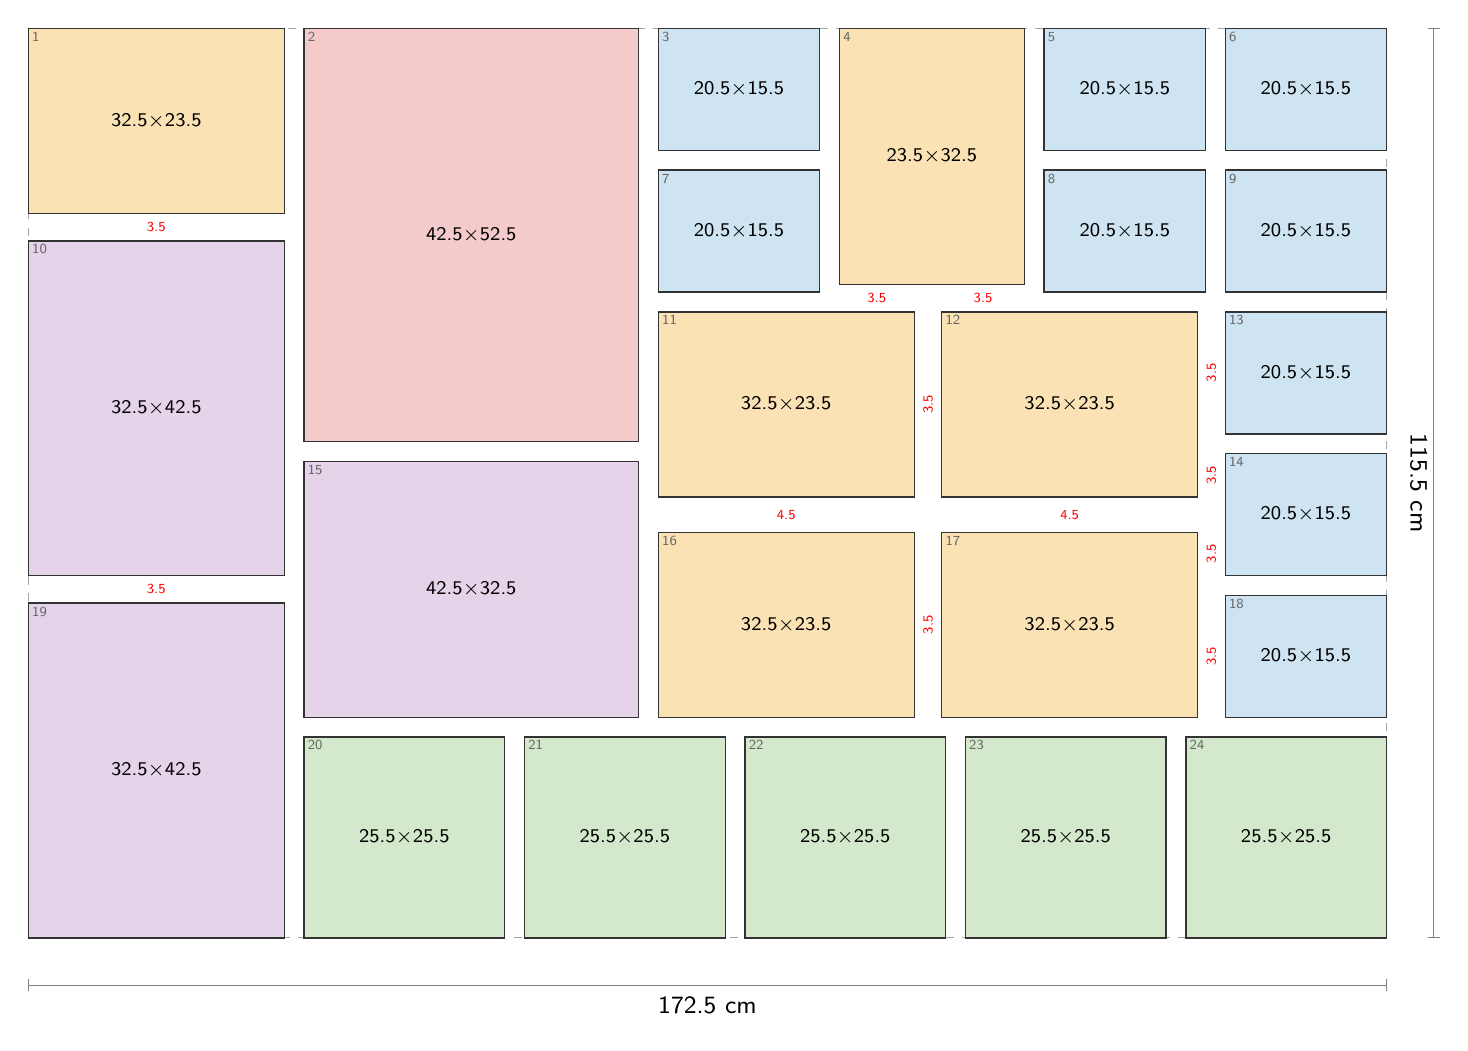
\begin{tikzpicture}[x=1mm, y=-1mm]
\draw[gray!70, dashed, line width=0.4pt] (0,0) rectangle (172.50,115.50);
\filldraw[fill=ft1, draw=black!80, line width=0.5pt] (0.00,0.00) rectangle (32.50,23.50);
\node[align=center, inner sep=0pt] at (16.25,11.75) {\scriptsize 32.5$\times$23.5};
\node[anchor=north west, inner sep=1.2pt, font=\tiny, text=black!60] at (0.00,0.00) {1};
\filldraw[fill=ft4, draw=black!80, line width=0.5pt] (35.00,0.00) rectangle (77.50,52.50);
\node[align=center, inner sep=0pt] at (56.25,26.25) {\scriptsize 42.5$\times$52.5};
\node[anchor=north west, inner sep=1.2pt, font=\tiny, text=black!60] at (35.00,0.00) {2};
\filldraw[fill=ft0, draw=black!80, line width=0.5pt] (80.00,0.00) rectangle (100.50,15.50);
\node[align=center, inner sep=0pt] at (90.25,7.75) {\scriptsize 20.5$\times$15.5};
\node[anchor=north west, inner sep=1.2pt, font=\tiny, text=black!60] at (80.00,0.00) {3};
\filldraw[fill=ft1, draw=black!80, line width=0.5pt] (103.00,0.00) rectangle (126.50,32.50);
\node[align=center, inner sep=0pt] at (114.75,16.25) {\scriptsize 23.5$\times$32.5};
\node[anchor=north west, inner sep=1.2pt, font=\tiny, text=black!60] at (103.00,0.00) {4};
\filldraw[fill=ft0, draw=black!80, line width=0.5pt] (129.00,0.00) rectangle (149.50,15.50);
\node[align=center, inner sep=0pt] at (139.25,7.75) {\scriptsize 20.5$\times$15.5};
\node[anchor=north west, inner sep=1.2pt, font=\tiny, text=black!60] at (129.00,0.00) {5};
\filldraw[fill=ft0, draw=black!80, line width=0.5pt] (152.00,0.00) rectangle (172.50,15.50);
\node[align=center, inner sep=0pt] at (162.25,7.75) {\scriptsize 20.5$\times$15.5};
\node[anchor=north west, inner sep=1.2pt, font=\tiny, text=black!60] at (152.00,0.00) {6};
\filldraw[fill=ft0, draw=black!80, line width=0.5pt] (80.00,18.00) rectangle (100.50,33.50);
\node[align=center, inner sep=0pt] at (90.25,25.75) {\scriptsize 20.5$\times$15.5};
\node[anchor=north west, inner sep=1.2pt, font=\tiny, text=black!60] at (80.00,18.00) {7};
\filldraw[fill=ft0, draw=black!80, line width=0.5pt] (129.00,18.00) rectangle (149.50,33.50);
\node[align=center, inner sep=0pt] at (139.25,25.75) {\scriptsize 20.5$\times$15.5};
\node[anchor=north west, inner sep=1.2pt, font=\tiny, text=black!60] at (129.00,18.00) {8};
\filldraw[fill=ft0, draw=black!80, line width=0.5pt] (152.00,18.00) rectangle (172.50,33.50);
\node[align=center, inner sep=0pt] at (162.25,25.75) {\scriptsize 20.5$\times$15.5};
\node[anchor=north west, inner sep=1.2pt, font=\tiny, text=black!60] at (152.00,18.00) {9};
\filldraw[fill=ft3, draw=black!80, line width=0.5pt] (0.00,27.00) rectangle (32.50,69.50);
\node[align=center, inner sep=0pt] at (16.25,48.25) {\scriptsize 32.5$\times$42.5};
\node[anchor=north west, inner sep=1.2pt, font=\tiny, text=black!60] at (0.00,27.00) {10};
\filldraw[fill=ft1, draw=black!80, line width=0.5pt] (80.00,36.00) rectangle (112.50,59.50);
\node[align=center, inner sep=0pt] at (96.25,47.75) {\scriptsize 32.5$\times$23.5};
\node[anchor=north west, inner sep=1.2pt, font=\tiny, text=black!60] at (80.00,36.00) {11};
\filldraw[fill=ft1, draw=black!80, line width=0.5pt] (116.00,36.00) rectangle (148.50,59.50);
\node[align=center, inner sep=0pt] at (132.25,47.75) {\scriptsize 32.5$\times$23.5};
\node[anchor=north west, inner sep=1.2pt, font=\tiny, text=black!60] at (116.00,36.00) {12};
\filldraw[fill=ft0, draw=black!80, line width=0.5pt] (152.00,36.00) rectangle (172.50,51.50);
\node[align=center, inner sep=0pt] at (162.25,43.75) {\scriptsize 20.5$\times$15.5};
\node[anchor=north west, inner sep=1.2pt, font=\tiny, text=black!60] at (152.00,36.00) {13};
\filldraw[fill=ft0, draw=black!80, line width=0.5pt] (152.00,54.00) rectangle (172.50,69.50);
\node[align=center, inner sep=0pt] at (162.25,61.75) {\scriptsize 20.5$\times$15.5};
\node[anchor=north west, inner sep=1.2pt, font=\tiny, text=black!60] at (152.00,54.00) {14};
\filldraw[fill=ft3, draw=black!80, line width=0.5pt] (35.00,55.00) rectangle (77.50,87.50);
\node[align=center, inner sep=0pt] at (56.25,71.25) {\scriptsize 42.5$\times$32.5};
\node[anchor=north west, inner sep=1.2pt, font=\tiny, text=black!60] at (35.00,55.00) {15};
\filldraw[fill=ft1, draw=black!80, line width=0.5pt] (80.00,64.00) rectangle (112.50,87.50);
\node[align=center, inner sep=0pt] at (96.25,75.75) {\scriptsize 32.5$\times$23.5};
\node[anchor=north west, inner sep=1.2pt, font=\tiny, text=black!60] at (80.00,64.00) {16};
\filldraw[fill=ft1, draw=black!80, line width=0.5pt] (116.00,64.00) rectangle (148.50,87.50);
\node[align=center, inner sep=0pt] at (132.25,75.75) {\scriptsize 32.5$\times$23.5};
\node[anchor=north west, inner sep=1.2pt, font=\tiny, text=black!60] at (116.00,64.00) {17};
\filldraw[fill=ft0, draw=black!80, line width=0.5pt] (152.00,72.00) rectangle (172.50,87.50);
\node[align=center, inner sep=0pt] at (162.25,79.75) {\scriptsize 20.5$\times$15.5};
\node[anchor=north west, inner sep=1.2pt, font=\tiny, text=black!60] at (152.00,72.00) {18};
\filldraw[fill=ft3, draw=black!80, line width=0.5pt] (0.00,73.00) rectangle (32.50,115.50);
\node[align=center, inner sep=0pt] at (16.25,94.25) {\scriptsize 32.5$\times$42.5};
\node[anchor=north west, inner sep=1.2pt, font=\tiny, text=black!60] at (0.00,73.00) {19};
\filldraw[fill=ft2, draw=black!80, line width=0.5pt] (35.00,90.00) rectangle (60.50,115.50);
\node[align=center, inner sep=0pt] at (47.75,102.75) {\scriptsize 25.5$\times$25.5};
\node[anchor=north west, inner sep=1.2pt, font=\tiny, text=black!60] at (35.00,90.00) {20};
\filldraw[fill=ft2, draw=black!80, line width=0.5pt] (63.00,90.00) rectangle (88.50,115.50);
\node[align=center, inner sep=0pt] at (75.75,102.75) {\scriptsize 25.5$\times$25.5};
\node[anchor=north west, inner sep=1.2pt, font=\tiny, text=black!60] at (63.00,90.00) {21};
\filldraw[fill=ft2, draw=black!80, line width=0.5pt] (91.00,90.00) rectangle (116.50,115.50);
\node[align=center, inner sep=0pt] at (103.75,102.75) {\scriptsize 25.5$\times$25.5};
\node[anchor=north west, inner sep=1.2pt, font=\tiny, text=black!60] at (91.00,90.00) {22};
\filldraw[fill=ft2, draw=black!80, line width=0.5pt] (119.00,90.00) rectangle (144.50,115.50);
\node[align=center, inner sep=0pt] at (131.75,102.75) {\scriptsize 25.5$\times$25.5};
\node[anchor=north west, inner sep=1.2pt, font=\tiny, text=black!60] at (119.00,90.00) {23};
\filldraw[fill=ft2, draw=black!80, line width=0.5pt] (147.00,90.00) rectangle (172.50,115.50);
\node[align=center, inner sep=0pt] at (159.75,102.75) {\scriptsize 25.5$\times$25.5};
\node[anchor=north west, inner sep=1.2pt, font=\tiny, text=black!60] at (147.00,90.00) {24};
\node[font=\tiny, text=red, fill=white, inner sep=0.3pt] at (16.25,25.25) {3.5};
\node[font=\tiny, text=red, fill=white, inner sep=0.3pt] at (107.75,34.25) {3.5};
\node[font=\tiny, text=red, fill=white, inner sep=0.3pt] at (121.25,34.25) {3.5};
\node[font=\tiny, text=red, fill=white, inner sep=0.3pt] at (16.25,71.25) {3.5};
\node[font=\tiny, text=red, fill=white, inner sep=0.3pt, rotate=90] at (114.25,47.75) {3.5};
\node[font=\tiny, text=red, fill=white, inner sep=0.3pt] at (96.25,61.75) {4.5};
\node[font=\tiny, text=red, fill=white, inner sep=0.3pt, rotate=90] at (150.25,43.75) {3.5};
\node[font=\tiny, text=red, fill=white, inner sep=0.3pt, rotate=90] at (150.25,56.75) {3.5};
\node[font=\tiny, text=red, fill=white, inner sep=0.3pt] at (132.25,61.75) {4.5};
\node[font=\tiny, text=red, fill=white, inner sep=0.3pt, rotate=90] at (114.25,75.75) {3.5};
\node[font=\tiny, text=red, fill=white, inner sep=0.3pt, rotate=90] at (150.25,66.75) {3.5};
\node[font=\tiny, text=red, fill=white, inner sep=0.3pt, rotate=90] at (150.25,79.75) {3.5};
\draw[Bar-Bar, gray] (0,121.50) -- (172.50,121.50) node[midway, below=1pt, font=\small, text=black] {172.5 cm};
\draw[Bar-Bar, gray] (178.50,0) -- (178.50,115.50) node[midway, right=1pt, font=\small, text=black, rotate=-90, anchor=north] {115.5 cm};
\end{tikzpicture}\\[4pt]
{\scriptsize Scale 1:10 (1 mm = 1 cm). Red numbers mark gaps that deviate from the nominal gap by more than 0.25 cm. Small grey numbers index the coordinate table.}
\end{minipage}\hfill
\begin{minipage}[t]{0.25\textwidth}\vspace{0pt}
\small
\begin{tabular}{@{}l l@{}}
\toprule
Outer size & 172.5 $\times$ 115.5 cm \\
Nominal gap & 2.5 cm \\
Actual gaps & 2.5 -- 4.5 cm \\
Max.\ deviation & 2.0 cm \\
Mean deviation & 0.30 cm \\
Border notches & none \\
Corners filled & 4 / 4 \\
Frames used & 24 of 28 \\
\bottomrule
\end{tabular}

\vspace{8pt}
\scriptsize
\begin{tabular}{@{}c l l r r@{}}
\toprule
 & outer w $\times$ h (cm) & & used & have \\
\midrule
\tikz[baseline=-0.6ex]\fill[ft0,draw=black!60] (0,0) rectangle (1.2ex,1.2ex); & 20.5$\times$15.5 & L & 9 & 9 \\
\tikz[baseline=-0.6ex]\fill[ft0,draw=black!60] (0,0) rectangle (1.2ex,1.2ex); & 15.5$\times$20.5 & P & 0 & 2 \\
\tikz[baseline=-0.6ex]\fill[ft3,draw=black!60] (0,0) rectangle (1.2ex,1.2ex); & 32.5$\times$42.5 & P & 2 & 2 \\
\tikz[baseline=-0.6ex]\fill[ft3,draw=black!60] (0,0) rectangle (1.2ex,1.2ex); & 42.5$\times$32.5 & L & 1 & 1 \\
\tikz[baseline=-0.6ex]\fill[ft1,draw=black!60] (0,0) rectangle (1.2ex,1.2ex); & 32.5$\times$23.5 & L & 5 & 5 \\
\tikz[baseline=-0.6ex]\fill[ft1,draw=black!60] (0,0) rectangle (1.2ex,1.2ex); & 23.5$\times$32.5 & P & 1 & 1 \\
\tikz[baseline=-0.6ex]\fill[ft2,draw=black!60] (0,0) rectangle (1.2ex,1.2ex); & 25.5$\times$25.5 &  & 5 & 5 \\
\tikz[baseline=-0.6ex]\fill[ft4,draw=black!60] (0,0) rectangle (1.2ex,1.2ex); & 42.5$\times$52.5 & P & 1 & 1 \\
\tikz[baseline=-0.6ex]\fill[ft4,draw=black!60] (0,0) rectangle (1.2ex,1.2ex); & 52.5$\times$42.5 & L & 0 & 2 \\
\bottomrule
\end{tabular}

\vspace{8pt}
{\bfseries Positions} (top-left corner, cm)\\[2pt]
\tiny
\begin{tabular}{@{}r l r r@{}}
\toprule
\# & frame w $\times$ h & x & y \\
\midrule
1 & 32.5 $\times$ 23.5 & 0.0 & 0.0 \\
2 & 42.5 $\times$ 52.5 & 35.0 & 0.0 \\
3 & 20.5 $\times$ 15.5 & 80.0 & 0.0 \\
4 & 23.5 $\times$ 32.5 & 103.0 & 0.0 \\
5 & 20.5 $\times$ 15.5 & 129.0 & 0.0 \\
6 & 20.5 $\times$ 15.5 & 152.0 & 0.0 \\
7 & 20.5 $\times$ 15.5 & 80.0 & 18.0 \\
8 & 20.5 $\times$ 15.5 & 129.0 & 18.0 \\
9 & 20.5 $\times$ 15.5 & 152.0 & 18.0 \\
10 & 32.5 $\times$ 42.5 & 0.0 & 27.0 \\
11 & 32.5 $\times$ 23.5 & 80.0 & 36.0 \\
12 & 32.5 $\times$ 23.5 & 116.0 & 36.0 \\
13 & 20.5 $\times$ 15.5 & 152.0 & 36.0 \\
14 & 20.5 $\times$ 15.5 & 152.0 & 54.0 \\
15 & 42.5 $\times$ 32.5 & 35.0 & 55.0 \\
16 & 32.5 $\times$ 23.5 & 80.0 & 64.0 \\
17 & 32.5 $\times$ 23.5 & 116.0 & 64.0 \\
18 & 20.5 $\times$ 15.5 & 152.0 & 72.0 \\
19 & 32.5 $\times$ 42.5 & 0.0 & 73.0 \\
20 & 25.5 $\times$ 25.5 & 35.0 & 90.0 \\
21 & 25.5 $\times$ 25.5 & 63.0 & 90.0 \\
22 & 25.5 $\times$ 25.5 & 91.0 & 90.0 \\
23 & 25.5 $\times$ 25.5 & 119.0 & 90.0 \\
24 & 25.5 $\times$ 25.5 & 147.0 & 90.0 \\
\bottomrule
\end{tabular}
\end{minipage}
\clearpage

\begin{minipage}[t]{0.74\textwidth}\vspace{0pt}
{\LARGE\bfseries Layout 2}\hspace{1.5em}{\large 181.5 $\times$ 113.5 cm \quad gap 1.5 cm \quad 23 frames}\\[8pt]
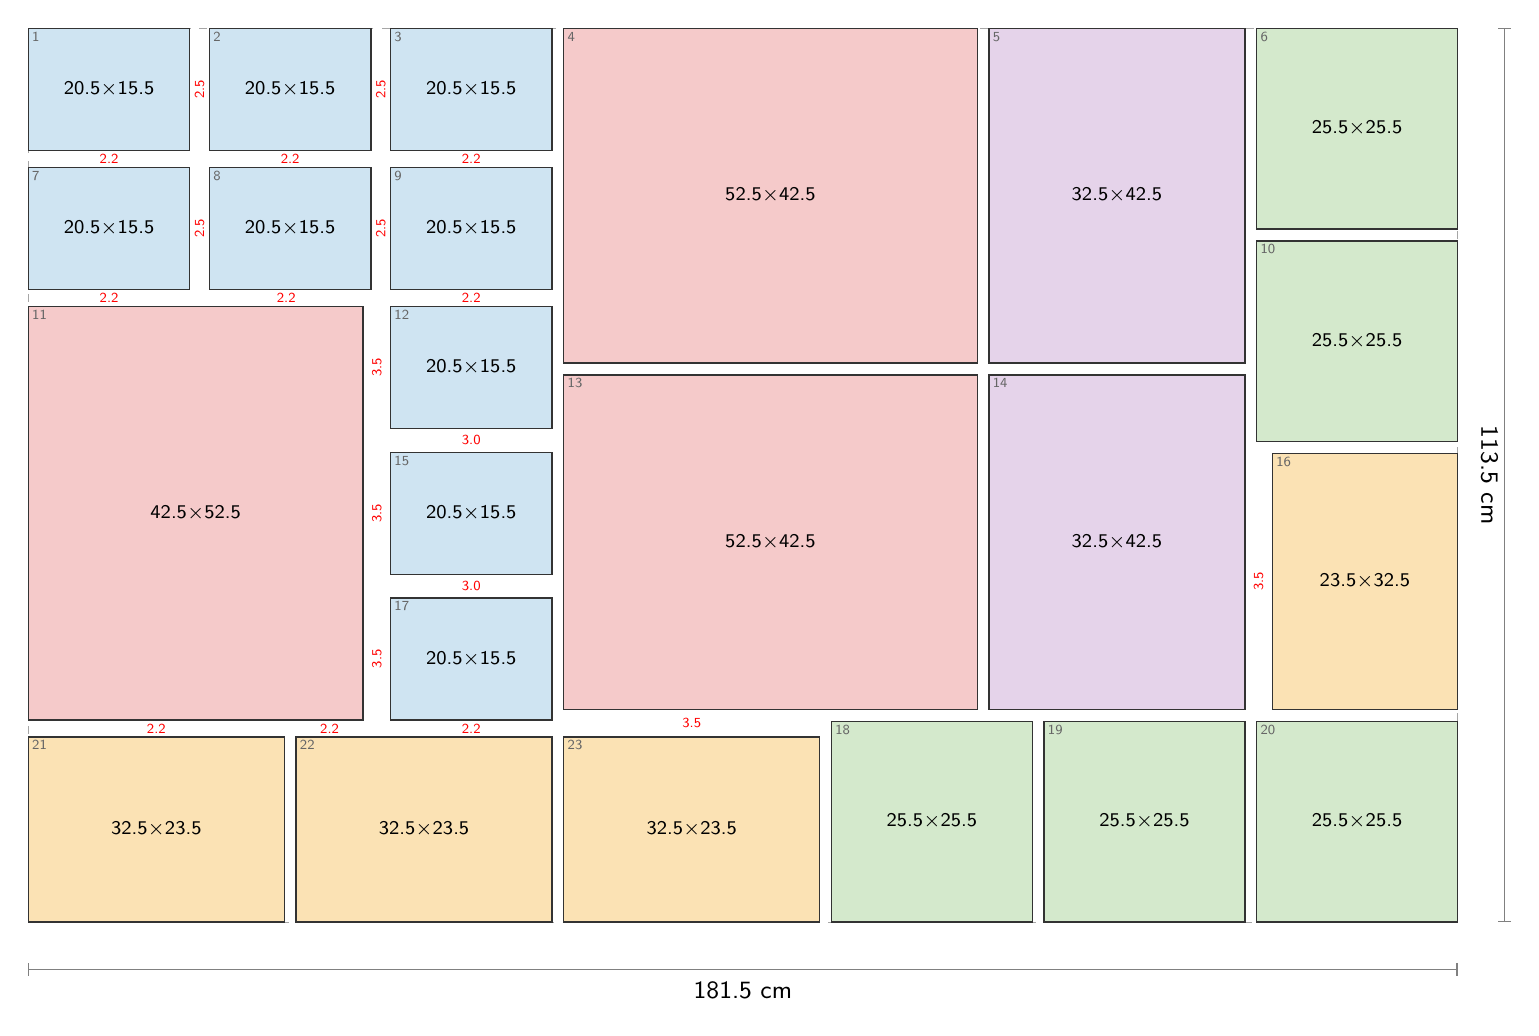
\begin{tikzpicture}[x=1mm, y=-1mm]
\draw[gray!70, dashed, line width=0.4pt] (0,0) rectangle (181.50,113.50);
\filldraw[fill=ft0, draw=black!80, line width=0.5pt] (0.00,0.00) rectangle (20.50,15.50);
\node[align=center, inner sep=0pt] at (10.25,7.75) {\scriptsize 20.5$\times$15.5};
\node[anchor=north west, inner sep=1.2pt, font=\tiny, text=black!60] at (0.00,0.00) {1};
\filldraw[fill=ft0, draw=black!80, line width=0.5pt] (23.00,0.00) rectangle (43.50,15.50);
\node[align=center, inner sep=0pt] at (33.25,7.75) {\scriptsize 20.5$\times$15.5};
\node[anchor=north west, inner sep=1.2pt, font=\tiny, text=black!60] at (23.00,0.00) {2};
\filldraw[fill=ft0, draw=black!80, line width=0.5pt] (46.00,0.00) rectangle (66.50,15.50);
\node[align=center, inner sep=0pt] at (56.25,7.75) {\scriptsize 20.5$\times$15.5};
\node[anchor=north west, inner sep=1.2pt, font=\tiny, text=black!60] at (46.00,0.00) {3};
\filldraw[fill=ft4, draw=black!80, line width=0.5pt] (68.00,0.00) rectangle (120.50,42.50);
\node[align=center, inner sep=0pt] at (94.25,21.25) {\scriptsize 52.5$\times$42.5};
\node[anchor=north west, inner sep=1.2pt, font=\tiny, text=black!60] at (68.00,0.00) {4};
\filldraw[fill=ft3, draw=black!80, line width=0.5pt] (122.00,0.00) rectangle (154.50,42.50);
\node[align=center, inner sep=0pt] at (138.25,21.25) {\scriptsize 32.5$\times$42.5};
\node[anchor=north west, inner sep=1.2pt, font=\tiny, text=black!60] at (122.00,0.00) {5};
\filldraw[fill=ft2, draw=black!80, line width=0.5pt] (156.00,0.00) rectangle (181.50,25.50);
\node[align=center, inner sep=0pt] at (168.75,12.75) {\scriptsize 25.5$\times$25.5};
\node[anchor=north west, inner sep=1.2pt, font=\tiny, text=black!60] at (156.00,0.00) {6};
\filldraw[fill=ft0, draw=black!80, line width=0.5pt] (0.00,17.67) rectangle (20.50,33.17);
\node[align=center, inner sep=0pt] at (10.25,25.42) {\scriptsize 20.5$\times$15.5};
\node[anchor=north west, inner sep=1.2pt, font=\tiny, text=black!60] at (0.00,17.67) {7};
\filldraw[fill=ft0, draw=black!80, line width=0.5pt] (23.00,17.67) rectangle (43.50,33.17);
\node[align=center, inner sep=0pt] at (33.25,25.42) {\scriptsize 20.5$\times$15.5};
\node[anchor=north west, inner sep=1.2pt, font=\tiny, text=black!60] at (23.00,17.67) {8};
\filldraw[fill=ft0, draw=black!80, line width=0.5pt] (46.00,17.67) rectangle (66.50,33.17);
\node[align=center, inner sep=0pt] at (56.25,25.42) {\scriptsize 20.5$\times$15.5};
\node[anchor=north west, inner sep=1.2pt, font=\tiny, text=black!60] at (46.00,17.67) {9};
\filldraw[fill=ft2, draw=black!80, line width=0.5pt] (156.00,27.00) rectangle (181.50,52.50);
\node[align=center, inner sep=0pt] at (168.75,39.75) {\scriptsize 25.5$\times$25.5};
\node[anchor=north west, inner sep=1.2pt, font=\tiny, text=black!60] at (156.00,27.00) {10};
\filldraw[fill=ft4, draw=black!80, line width=0.5pt] (0.00,35.33) rectangle (42.50,87.83);
\node[align=center, inner sep=0pt] at (21.25,61.58) {\scriptsize 42.5$\times$52.5};
\node[anchor=north west, inner sep=1.2pt, font=\tiny, text=black!60] at (0.00,35.33) {11};
\filldraw[fill=ft0, draw=black!80, line width=0.5pt] (46.00,35.33) rectangle (66.50,50.83);
\node[align=center, inner sep=0pt] at (56.25,43.08) {\scriptsize 20.5$\times$15.5};
\node[anchor=north west, inner sep=1.2pt, font=\tiny, text=black!60] at (46.00,35.33) {12};
\filldraw[fill=ft4, draw=black!80, line width=0.5pt] (68.00,44.00) rectangle (120.50,86.50);
\node[align=center, inner sep=0pt] at (94.25,65.25) {\scriptsize 52.5$\times$42.5};
\node[anchor=north west, inner sep=1.2pt, font=\tiny, text=black!60] at (68.00,44.00) {13};
\filldraw[fill=ft3, draw=black!80, line width=0.5pt] (122.00,44.00) rectangle (154.50,86.50);
\node[align=center, inner sep=0pt] at (138.25,65.25) {\scriptsize 32.5$\times$42.5};
\node[anchor=north west, inner sep=1.2pt, font=\tiny, text=black!60] at (122.00,44.00) {14};
\filldraw[fill=ft0, draw=black!80, line width=0.5pt] (46.00,53.83) rectangle (66.50,69.33);
\node[align=center, inner sep=0pt] at (56.25,61.58) {\scriptsize 20.5$\times$15.5};
\node[anchor=north west, inner sep=1.2pt, font=\tiny, text=black!60] at (46.00,53.83) {15};
\filldraw[fill=ft1, draw=black!80, line width=0.5pt] (158.00,54.00) rectangle (181.50,86.50);
\node[align=center, inner sep=0pt] at (169.75,70.25) {\scriptsize 23.5$\times$32.5};
\node[anchor=north west, inner sep=1.2pt, font=\tiny, text=black!60] at (158.00,54.00) {16};
\filldraw[fill=ft0, draw=black!80, line width=0.5pt] (46.00,72.33) rectangle (66.50,87.83);
\node[align=center, inner sep=0pt] at (56.25,80.08) {\scriptsize 20.5$\times$15.5};
\node[anchor=north west, inner sep=1.2pt, font=\tiny, text=black!60] at (46.00,72.33) {17};
\filldraw[fill=ft2, draw=black!80, line width=0.5pt] (102.00,88.00) rectangle (127.50,113.50);
\node[align=center, inner sep=0pt] at (114.75,100.75) {\scriptsize 25.5$\times$25.5};
\node[anchor=north west, inner sep=1.2pt, font=\tiny, text=black!60] at (102.00,88.00) {18};
\filldraw[fill=ft2, draw=black!80, line width=0.5pt] (129.00,88.00) rectangle (154.50,113.50);
\node[align=center, inner sep=0pt] at (141.75,100.75) {\scriptsize 25.5$\times$25.5};
\node[anchor=north west, inner sep=1.2pt, font=\tiny, text=black!60] at (129.00,88.00) {19};
\filldraw[fill=ft2, draw=black!80, line width=0.5pt] (156.00,88.00) rectangle (181.50,113.50);
\node[align=center, inner sep=0pt] at (168.75,100.75) {\scriptsize 25.5$\times$25.5};
\node[anchor=north west, inner sep=1.2pt, font=\tiny, text=black!60] at (156.00,88.00) {20};
\filldraw[fill=ft1, draw=black!80, line width=0.5pt] (0.00,90.00) rectangle (32.50,113.50);
\node[align=center, inner sep=0pt] at (16.25,101.75) {\scriptsize 32.5$\times$23.5};
\node[anchor=north west, inner sep=1.2pt, font=\tiny, text=black!60] at (0.00,90.00) {21};
\filldraw[fill=ft1, draw=black!80, line width=0.5pt] (34.00,90.00) rectangle (66.50,113.50);
\node[align=center, inner sep=0pt] at (50.25,101.75) {\scriptsize 32.5$\times$23.5};
\node[anchor=north west, inner sep=1.2pt, font=\tiny, text=black!60] at (34.00,90.00) {22};
\filldraw[fill=ft1, draw=black!80, line width=0.5pt] (68.00,90.00) rectangle (100.50,113.50);
\node[align=center, inner sep=0pt] at (84.25,101.75) {\scriptsize 32.5$\times$23.5};
\node[anchor=north west, inner sep=1.2pt, font=\tiny, text=black!60] at (68.00,90.00) {23};
\node[font=\tiny, text=red, fill=white, inner sep=0.3pt, rotate=90] at (21.75,7.75) {2.5};
\node[font=\tiny, text=red, fill=white, inner sep=0.3pt] at (10.25,16.58) {2.2};
\node[font=\tiny, text=red, fill=white, inner sep=0.3pt, rotate=90] at (44.75,7.75) {2.5};
\node[font=\tiny, text=red, fill=white, inner sep=0.3pt] at (33.25,16.58) {2.2};
\node[font=\tiny, text=red, fill=white, inner sep=0.3pt] at (56.25,16.58) {2.2};
\node[font=\tiny, text=red, fill=white, inner sep=0.3pt, rotate=90] at (21.75,25.42) {2.5};
\node[font=\tiny, text=red, fill=white, inner sep=0.3pt] at (10.25,34.25) {2.2};
\node[font=\tiny, text=red, fill=white, inner sep=0.3pt, rotate=90] at (44.75,25.42) {2.5};
\node[font=\tiny, text=red, fill=white, inner sep=0.3pt] at (32.75,34.25) {2.2};
\node[font=\tiny, text=red, fill=white, inner sep=0.3pt] at (56.25,34.25) {2.2};
\node[font=\tiny, text=red, fill=white, inner sep=0.3pt, rotate=90] at (44.25,43.08) {3.5};
\node[font=\tiny, text=red, fill=white, inner sep=0.3pt, rotate=90] at (44.25,61.58) {3.5};
\node[font=\tiny, text=red, fill=white, inner sep=0.3pt, rotate=90] at (44.25,80.08) {3.5};
\node[font=\tiny, text=red, fill=white, inner sep=0.3pt] at (16.25,88.92) {2.2};
\node[font=\tiny, text=red, fill=white, inner sep=0.3pt] at (38.25,88.92) {2.2};
\node[font=\tiny, text=red, fill=white, inner sep=0.3pt] at (56.25,52.33) {3.0};
\node[font=\tiny, text=red, fill=white, inner sep=0.3pt] at (84.25,88.25) {3.5};
\node[font=\tiny, text=red, fill=white, inner sep=0.3pt, rotate=90] at (156.25,70.25) {3.5};
\node[font=\tiny, text=red, fill=white, inner sep=0.3pt] at (56.25,70.83) {3.0};
\node[font=\tiny, text=red, fill=white, inner sep=0.3pt] at (56.25,88.92) {2.2};
\draw[Bar-Bar, gray] (0,119.50) -- (181.50,119.50) node[midway, below=1pt, font=\small, text=black] {181.5 cm};
\draw[Bar-Bar, gray] (187.50,0) -- (187.50,113.50) node[midway, right=1pt, font=\small, text=black, rotate=-90, anchor=north] {113.5 cm};
\end{tikzpicture}\\[4pt]
{\scriptsize Scale 1:10 (1 mm = 1 cm). Red numbers mark gaps that deviate from the nominal gap by more than 0.25 cm. Small grey numbers index the coordinate table.}
\end{minipage}\hfill
\begin{minipage}[t]{0.25\textwidth}\vspace{0pt}
\small
\begin{tabular}{@{}l l@{}}
\toprule
Outer size & 181.5 $\times$ 113.5 cm \\
Nominal gap & 1.5 cm \\
Actual gaps & 1.5 -- 3.5 cm \\
Max.\ deviation & 2.0 cm \\
Mean deviation & 0.52 cm \\
Border notches & none \\
Corners filled & 4 / 4 \\
Frames used & 23 of 28 \\
\bottomrule
\end{tabular}

\vspace{8pt}
\scriptsize
\begin{tabular}{@{}c l l r r@{}}
\toprule
 & outer w $\times$ h (cm) & & used & have \\
\midrule
\tikz[baseline=-0.6ex]\fill[ft0,draw=black!60] (0,0) rectangle (1.2ex,1.2ex); & 20.5$\times$15.5 & L & 9 & 9 \\
\tikz[baseline=-0.6ex]\fill[ft0,draw=black!60] (0,0) rectangle (1.2ex,1.2ex); & 15.5$\times$20.5 & P & 0 & 2 \\
\tikz[baseline=-0.6ex]\fill[ft3,draw=black!60] (0,0) rectangle (1.2ex,1.2ex); & 32.5$\times$42.5 & P & 2 & 2 \\
\tikz[baseline=-0.6ex]\fill[ft3,draw=black!60] (0,0) rectangle (1.2ex,1.2ex); & 42.5$\times$32.5 & L & 0 & 1 \\
\tikz[baseline=-0.6ex]\fill[ft1,draw=black!60] (0,0) rectangle (1.2ex,1.2ex); & 32.5$\times$23.5 & L & 3 & 5 \\
\tikz[baseline=-0.6ex]\fill[ft1,draw=black!60] (0,0) rectangle (1.2ex,1.2ex); & 23.5$\times$32.5 & P & 1 & 1 \\
\tikz[baseline=-0.6ex]\fill[ft2,draw=black!60] (0,0) rectangle (1.2ex,1.2ex); & 25.5$\times$25.5 &  & 5 & 5 \\
\tikz[baseline=-0.6ex]\fill[ft4,draw=black!60] (0,0) rectangle (1.2ex,1.2ex); & 42.5$\times$52.5 & P & 1 & 1 \\
\tikz[baseline=-0.6ex]\fill[ft4,draw=black!60] (0,0) rectangle (1.2ex,1.2ex); & 52.5$\times$42.5 & L & 2 & 2 \\
\bottomrule
\end{tabular}

\vspace{8pt}
{\bfseries Positions} (top-left corner, cm)\\[2pt]
\tiny
\begin{tabular}{@{}r l r r@{}}
\toprule
\# & frame w $\times$ h & x & y \\
\midrule
1 & 20.5 $\times$ 15.5 & 0.0 & 0.0 \\
2 & 20.5 $\times$ 15.5 & 23.0 & 0.0 \\
3 & 20.5 $\times$ 15.5 & 46.0 & 0.0 \\
4 & 52.5 $\times$ 42.5 & 68.0 & 0.0 \\
5 & 32.5 $\times$ 42.5 & 122.0 & 0.0 \\
6 & 25.5 $\times$ 25.5 & 156.0 & 0.0 \\
7 & 20.5 $\times$ 15.5 & 0.0 & 17.7 \\
8 & 20.5 $\times$ 15.5 & 23.0 & 17.7 \\
9 & 20.5 $\times$ 15.5 & 46.0 & 17.7 \\
10 & 25.5 $\times$ 25.5 & 156.0 & 27.0 \\
11 & 42.5 $\times$ 52.5 & 0.0 & 35.3 \\
12 & 20.5 $\times$ 15.5 & 46.0 & 35.3 \\
13 & 52.5 $\times$ 42.5 & 68.0 & 44.0 \\
14 & 32.5 $\times$ 42.5 & 122.0 & 44.0 \\
15 & 20.5 $\times$ 15.5 & 46.0 & 53.8 \\
16 & 23.5 $\times$ 32.5 & 158.0 & 54.0 \\
17 & 20.5 $\times$ 15.5 & 46.0 & 72.3 \\
18 & 25.5 $\times$ 25.5 & 102.0 & 88.0 \\
19 & 25.5 $\times$ 25.5 & 129.0 & 88.0 \\
20 & 25.5 $\times$ 25.5 & 156.0 & 88.0 \\
21 & 32.5 $\times$ 23.5 & 0.0 & 90.0 \\
22 & 32.5 $\times$ 23.5 & 34.0 & 90.0 \\
23 & 32.5 $\times$ 23.5 & 68.0 & 90.0 \\
\bottomrule
\end{tabular}
\end{minipage}
\clearpage

\begin{minipage}[t]{0.74\textwidth}\vspace{0pt}
{\LARGE\bfseries Layout 3}\hspace{1.5em}{\large 181.5 $\times$ 113.5 cm \quad gap 1.5 cm \quad 23 frames}\\[8pt]
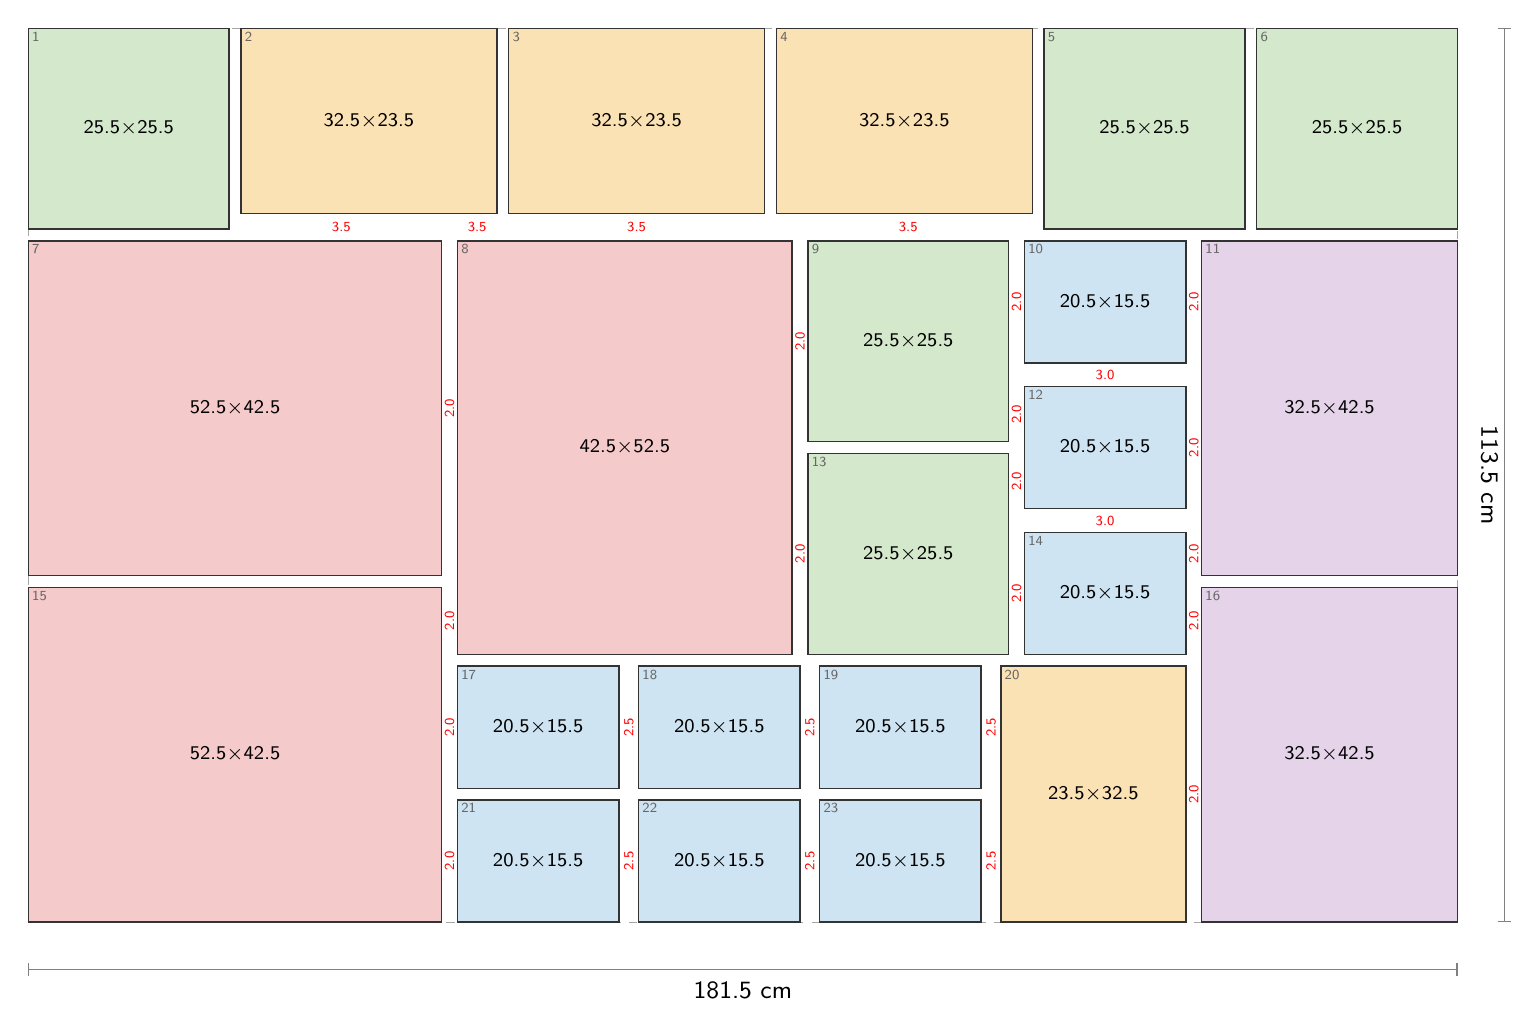
\begin{tikzpicture}[x=1mm, y=-1mm]
\draw[gray!70, dashed, line width=0.4pt] (0,0) rectangle (181.50,113.50);
\filldraw[fill=ft2, draw=black!80, line width=0.5pt] (0.00,0.00) rectangle (25.50,25.50);
\node[align=center, inner sep=0pt] at (12.75,12.75) {\scriptsize 25.5$\times$25.5};
\node[anchor=north west, inner sep=1.2pt, font=\tiny, text=black!60] at (0.00,0.00) {1};
\filldraw[fill=ft1, draw=black!80, line width=0.5pt] (27.00,0.00) rectangle (59.50,23.50);
\node[align=center, inner sep=0pt] at (43.25,11.75) {\scriptsize 32.5$\times$23.5};
\node[anchor=north west, inner sep=1.2pt, font=\tiny, text=black!60] at (27.00,0.00) {2};
\filldraw[fill=ft1, draw=black!80, line width=0.5pt] (61.00,0.00) rectangle (93.50,23.50);
\node[align=center, inner sep=0pt] at (77.25,11.75) {\scriptsize 32.5$\times$23.5};
\node[anchor=north west, inner sep=1.2pt, font=\tiny, text=black!60] at (61.00,0.00) {3};
\filldraw[fill=ft1, draw=black!80, line width=0.5pt] (95.00,0.00) rectangle (127.50,23.50);
\node[align=center, inner sep=0pt] at (111.25,11.75) {\scriptsize 32.5$\times$23.5};
\node[anchor=north west, inner sep=1.2pt, font=\tiny, text=black!60] at (95.00,0.00) {4};
\filldraw[fill=ft2, draw=black!80, line width=0.5pt] (129.00,0.00) rectangle (154.50,25.50);
\node[align=center, inner sep=0pt] at (141.75,12.75) {\scriptsize 25.5$\times$25.5};
\node[anchor=north west, inner sep=1.2pt, font=\tiny, text=black!60] at (129.00,0.00) {5};
\filldraw[fill=ft2, draw=black!80, line width=0.5pt] (156.00,0.00) rectangle (181.50,25.50);
\node[align=center, inner sep=0pt] at (168.75,12.75) {\scriptsize 25.5$\times$25.5};
\node[anchor=north west, inner sep=1.2pt, font=\tiny, text=black!60] at (156.00,0.00) {6};
\filldraw[fill=ft4, draw=black!80, line width=0.5pt] (0.00,27.00) rectangle (52.50,69.50);
\node[align=center, inner sep=0pt] at (26.25,48.25) {\scriptsize 52.5$\times$42.5};
\node[anchor=north west, inner sep=1.2pt, font=\tiny, text=black!60] at (0.00,27.00) {7};
\filldraw[fill=ft4, draw=black!80, line width=0.5pt] (54.50,27.00) rectangle (97.00,79.50);
\node[align=center, inner sep=0pt] at (75.75,53.25) {\scriptsize 42.5$\times$52.5};
\node[anchor=north west, inner sep=1.2pt, font=\tiny, text=black!60] at (54.50,27.00) {8};
\filldraw[fill=ft2, draw=black!80, line width=0.5pt] (99.00,27.00) rectangle (124.50,52.50);
\node[align=center, inner sep=0pt] at (111.75,39.75) {\scriptsize 25.5$\times$25.5};
\node[anchor=north west, inner sep=1.2pt, font=\tiny, text=black!60] at (99.00,27.00) {9};
\filldraw[fill=ft0, draw=black!80, line width=0.5pt] (126.50,27.00) rectangle (147.00,42.50);
\node[align=center, inner sep=0pt] at (136.75,34.75) {\scriptsize 20.5$\times$15.5};
\node[anchor=north west, inner sep=1.2pt, font=\tiny, text=black!60] at (126.50,27.00) {10};
\filldraw[fill=ft3, draw=black!80, line width=0.5pt] (149.00,27.00) rectangle (181.50,69.50);
\node[align=center, inner sep=0pt] at (165.25,48.25) {\scriptsize 32.5$\times$42.5};
\node[anchor=north west, inner sep=1.2pt, font=\tiny, text=black!60] at (149.00,27.00) {11};
\filldraw[fill=ft0, draw=black!80, line width=0.5pt] (126.50,45.50) rectangle (147.00,61.00);
\node[align=center, inner sep=0pt] at (136.75,53.25) {\scriptsize 20.5$\times$15.5};
\node[anchor=north west, inner sep=1.2pt, font=\tiny, text=black!60] at (126.50,45.50) {12};
\filldraw[fill=ft2, draw=black!80, line width=0.5pt] (99.00,54.00) rectangle (124.50,79.50);
\node[align=center, inner sep=0pt] at (111.75,66.75) {\scriptsize 25.5$\times$25.5};
\node[anchor=north west, inner sep=1.2pt, font=\tiny, text=black!60] at (99.00,54.00) {13};
\filldraw[fill=ft0, draw=black!80, line width=0.5pt] (126.50,64.00) rectangle (147.00,79.50);
\node[align=center, inner sep=0pt] at (136.75,71.75) {\scriptsize 20.5$\times$15.5};
\node[anchor=north west, inner sep=1.2pt, font=\tiny, text=black!60] at (126.50,64.00) {14};
\filldraw[fill=ft4, draw=black!80, line width=0.5pt] (0.00,71.00) rectangle (52.50,113.50);
\node[align=center, inner sep=0pt] at (26.25,92.25) {\scriptsize 52.5$\times$42.5};
\node[anchor=north west, inner sep=1.2pt, font=\tiny, text=black!60] at (0.00,71.00) {15};
\filldraw[fill=ft3, draw=black!80, line width=0.5pt] (149.00,71.00) rectangle (181.50,113.50);
\node[align=center, inner sep=0pt] at (165.25,92.25) {\scriptsize 32.5$\times$42.5};
\node[anchor=north west, inner sep=1.2pt, font=\tiny, text=black!60] at (149.00,71.00) {16};
\filldraw[fill=ft0, draw=black!80, line width=0.5pt] (54.50,81.00) rectangle (75.00,96.50);
\node[align=center, inner sep=0pt] at (64.75,88.75) {\scriptsize 20.5$\times$15.5};
\node[anchor=north west, inner sep=1.2pt, font=\tiny, text=black!60] at (54.50,81.00) {17};
\filldraw[fill=ft0, draw=black!80, line width=0.5pt] (77.50,81.00) rectangle (98.00,96.50);
\node[align=center, inner sep=0pt] at (87.75,88.75) {\scriptsize 20.5$\times$15.5};
\node[anchor=north west, inner sep=1.2pt, font=\tiny, text=black!60] at (77.50,81.00) {18};
\filldraw[fill=ft0, draw=black!80, line width=0.5pt] (100.50,81.00) rectangle (121.00,96.50);
\node[align=center, inner sep=0pt] at (110.75,88.75) {\scriptsize 20.5$\times$15.5};
\node[anchor=north west, inner sep=1.2pt, font=\tiny, text=black!60] at (100.50,81.00) {19};
\filldraw[fill=ft1, draw=black!80, line width=0.5pt] (123.50,81.00) rectangle (147.00,113.50);
\node[align=center, inner sep=0pt] at (135.25,97.25) {\scriptsize 23.5$\times$32.5};
\node[anchor=north west, inner sep=1.2pt, font=\tiny, text=black!60] at (123.50,81.00) {20};
\filldraw[fill=ft0, draw=black!80, line width=0.5pt] (54.50,98.00) rectangle (75.00,113.50);
\node[align=center, inner sep=0pt] at (64.75,105.75) {\scriptsize 20.5$\times$15.5};
\node[anchor=north west, inner sep=1.2pt, font=\tiny, text=black!60] at (54.50,98.00) {21};
\filldraw[fill=ft0, draw=black!80, line width=0.5pt] (77.50,98.00) rectangle (98.00,113.50);
\node[align=center, inner sep=0pt] at (87.75,105.75) {\scriptsize 20.5$\times$15.5};
\node[anchor=north west, inner sep=1.2pt, font=\tiny, text=black!60] at (77.50,98.00) {22};
\filldraw[fill=ft0, draw=black!80, line width=0.5pt] (100.50,98.00) rectangle (121.00,113.50);
\node[align=center, inner sep=0pt] at (110.75,105.75) {\scriptsize 20.5$\times$15.5};
\node[anchor=north west, inner sep=1.2pt, font=\tiny, text=black!60] at (100.50,98.00) {23};
\node[font=\tiny, text=red, fill=white, inner sep=0.3pt] at (39.75,25.25) {3.5};
\node[font=\tiny, text=red, fill=white, inner sep=0.3pt] at (57.00,25.25) {3.5};
\node[font=\tiny, text=red, fill=white, inner sep=0.3pt] at (77.25,25.25) {3.5};
\node[font=\tiny, text=red, fill=white, inner sep=0.3pt] at (111.75,25.25) {3.5};
\node[font=\tiny, text=red, fill=white, inner sep=0.3pt, rotate=90] at (53.50,48.25) {2.0};
\node[font=\tiny, text=red, fill=white, inner sep=0.3pt, rotate=90] at (98.00,39.75) {2.0};
\node[font=\tiny, text=red, fill=white, inner sep=0.3pt, rotate=90] at (98.00,66.75) {2.0};
\node[font=\tiny, text=red, fill=white, inner sep=0.3pt, rotate=90] at (125.50,34.75) {2.0};
\node[font=\tiny, text=red, fill=white, inner sep=0.3pt, rotate=90] at (125.50,49.00) {2.0};
\node[font=\tiny, text=red, fill=white, inner sep=0.3pt, rotate=90] at (148.00,34.75) {2.0};
\node[font=\tiny, text=red, fill=white, inner sep=0.3pt] at (136.75,44.00) {3.0};
\node[font=\tiny, text=red, fill=white, inner sep=0.3pt, rotate=90] at (148.00,53.25) {2.0};
\node[font=\tiny, text=red, fill=white, inner sep=0.3pt] at (136.75,62.50) {3.0};
\node[font=\tiny, text=red, fill=white, inner sep=0.3pt, rotate=90] at (125.50,57.50) {2.0};
\node[font=\tiny, text=red, fill=white, inner sep=0.3pt, rotate=90] at (125.50,71.75) {2.0};
\node[font=\tiny, text=red, fill=white, inner sep=0.3pt, rotate=90] at (148.00,66.75) {2.0};
\node[font=\tiny, text=red, fill=white, inner sep=0.3pt, rotate=90] at (148.00,75.25) {2.0};
\node[font=\tiny, text=red, fill=white, inner sep=0.3pt, rotate=90] at (53.50,75.25) {2.0};
\node[font=\tiny, text=red, fill=white, inner sep=0.3pt, rotate=90] at (53.50,88.75) {2.0};
\node[font=\tiny, text=red, fill=white, inner sep=0.3pt, rotate=90] at (53.50,105.75) {2.0};
\node[font=\tiny, text=red, fill=white, inner sep=0.3pt, rotate=90] at (76.25,88.75) {2.5};
\node[font=\tiny, text=red, fill=white, inner sep=0.3pt, rotate=90] at (99.25,88.75) {2.5};
\node[font=\tiny, text=red, fill=white, inner sep=0.3pt, rotate=90] at (122.25,88.75) {2.5};
\node[font=\tiny, text=red, fill=white, inner sep=0.3pt, rotate=90] at (148.00,97.25) {2.0};
\node[font=\tiny, text=red, fill=white, inner sep=0.3pt, rotate=90] at (76.25,105.75) {2.5};
\node[font=\tiny, text=red, fill=white, inner sep=0.3pt, rotate=90] at (99.25,105.75) {2.5};
\node[font=\tiny, text=red, fill=white, inner sep=0.3pt, rotate=90] at (122.25,105.75) {2.5};
\draw[Bar-Bar, gray] (0,119.50) -- (181.50,119.50) node[midway, below=1pt, font=\small, text=black] {181.5 cm};
\draw[Bar-Bar, gray] (187.50,0) -- (187.50,113.50) node[midway, right=1pt, font=\small, text=black, rotate=-90, anchor=north] {113.5 cm};
\end{tikzpicture}\\[4pt]
{\scriptsize Scale 1:10 (1 mm = 1 cm). Red numbers mark gaps that deviate from the nominal gap by more than 0.25 cm. Small grey numbers index the coordinate table.}
\end{minipage}\hfill
\begin{minipage}[t]{0.25\textwidth}\vspace{0pt}
\small
\begin{tabular}{@{}l l@{}}
\toprule
Outer size & 181.5 $\times$ 113.5 cm \\
Nominal gap & 1.5 cm \\
Actual gaps & 1.5 -- 3.5 cm \\
Max.\ deviation & 2.0 cm \\
Mean deviation & 0.53 cm \\
Border notches & none \\
Corners filled & 4 / 4 \\
Frames used & 23 of 28 \\
\bottomrule
\end{tabular}

\vspace{8pt}
\scriptsize
\begin{tabular}{@{}c l l r r@{}}
\toprule
 & outer w $\times$ h (cm) & & used & have \\
\midrule
\tikz[baseline=-0.6ex]\fill[ft0,draw=black!60] (0,0) rectangle (1.2ex,1.2ex); & 20.5$\times$15.5 & L & 9 & 9 \\
\tikz[baseline=-0.6ex]\fill[ft0,draw=black!60] (0,0) rectangle (1.2ex,1.2ex); & 15.5$\times$20.5 & P & 0 & 2 \\
\tikz[baseline=-0.6ex]\fill[ft3,draw=black!60] (0,0) rectangle (1.2ex,1.2ex); & 32.5$\times$42.5 & P & 2 & 2 \\
\tikz[baseline=-0.6ex]\fill[ft3,draw=black!60] (0,0) rectangle (1.2ex,1.2ex); & 42.5$\times$32.5 & L & 0 & 1 \\
\tikz[baseline=-0.6ex]\fill[ft1,draw=black!60] (0,0) rectangle (1.2ex,1.2ex); & 32.5$\times$23.5 & L & 3 & 5 \\
\tikz[baseline=-0.6ex]\fill[ft1,draw=black!60] (0,0) rectangle (1.2ex,1.2ex); & 23.5$\times$32.5 & P & 1 & 1 \\
\tikz[baseline=-0.6ex]\fill[ft2,draw=black!60] (0,0) rectangle (1.2ex,1.2ex); & 25.5$\times$25.5 &  & 5 & 5 \\
\tikz[baseline=-0.6ex]\fill[ft4,draw=black!60] (0,0) rectangle (1.2ex,1.2ex); & 42.5$\times$52.5 & P & 1 & 1 \\
\tikz[baseline=-0.6ex]\fill[ft4,draw=black!60] (0,0) rectangle (1.2ex,1.2ex); & 52.5$\times$42.5 & L & 2 & 2 \\
\bottomrule
\end{tabular}

\vspace{8pt}
{\bfseries Positions} (top-left corner, cm)\\[2pt]
\tiny
\begin{tabular}{@{}r l r r@{}}
\toprule
\# & frame w $\times$ h & x & y \\
\midrule
1 & 25.5 $\times$ 25.5 & 0.0 & 0.0 \\
2 & 32.5 $\times$ 23.5 & 27.0 & 0.0 \\
3 & 32.5 $\times$ 23.5 & 61.0 & 0.0 \\
4 & 32.5 $\times$ 23.5 & 95.0 & 0.0 \\
5 & 25.5 $\times$ 25.5 & 129.0 & 0.0 \\
6 & 25.5 $\times$ 25.5 & 156.0 & 0.0 \\
7 & 52.5 $\times$ 42.5 & 0.0 & 27.0 \\
8 & 42.5 $\times$ 52.5 & 54.5 & 27.0 \\
9 & 25.5 $\times$ 25.5 & 99.0 & 27.0 \\
10 & 20.5 $\times$ 15.5 & 126.5 & 27.0 \\
11 & 32.5 $\times$ 42.5 & 149.0 & 27.0 \\
12 & 20.5 $\times$ 15.5 & 126.5 & 45.5 \\
13 & 25.5 $\times$ 25.5 & 99.0 & 54.0 \\
14 & 20.5 $\times$ 15.5 & 126.5 & 64.0 \\
15 & 52.5 $\times$ 42.5 & 0.0 & 71.0 \\
16 & 32.5 $\times$ 42.5 & 149.0 & 71.0 \\
17 & 20.5 $\times$ 15.5 & 54.5 & 81.0 \\
18 & 20.5 $\times$ 15.5 & 77.5 & 81.0 \\
19 & 20.5 $\times$ 15.5 & 100.5 & 81.0 \\
20 & 23.5 $\times$ 32.5 & 123.5 & 81.0 \\
21 & 20.5 $\times$ 15.5 & 54.5 & 98.0 \\
22 & 20.5 $\times$ 15.5 & 77.5 & 98.0 \\
23 & 20.5 $\times$ 15.5 & 100.5 & 98.0 \\
\bottomrule
\end{tabular}
\end{minipage}
\clearpage

\begin{minipage}[t]{0.74\textwidth}\vspace{0pt}
{\LARGE\bfseries Layout 4}\hspace{1.5em}{\large 189.5 $\times$ 109.5 cm \quad gap 3.5 cm \quad 22 frames}\\[8pt]
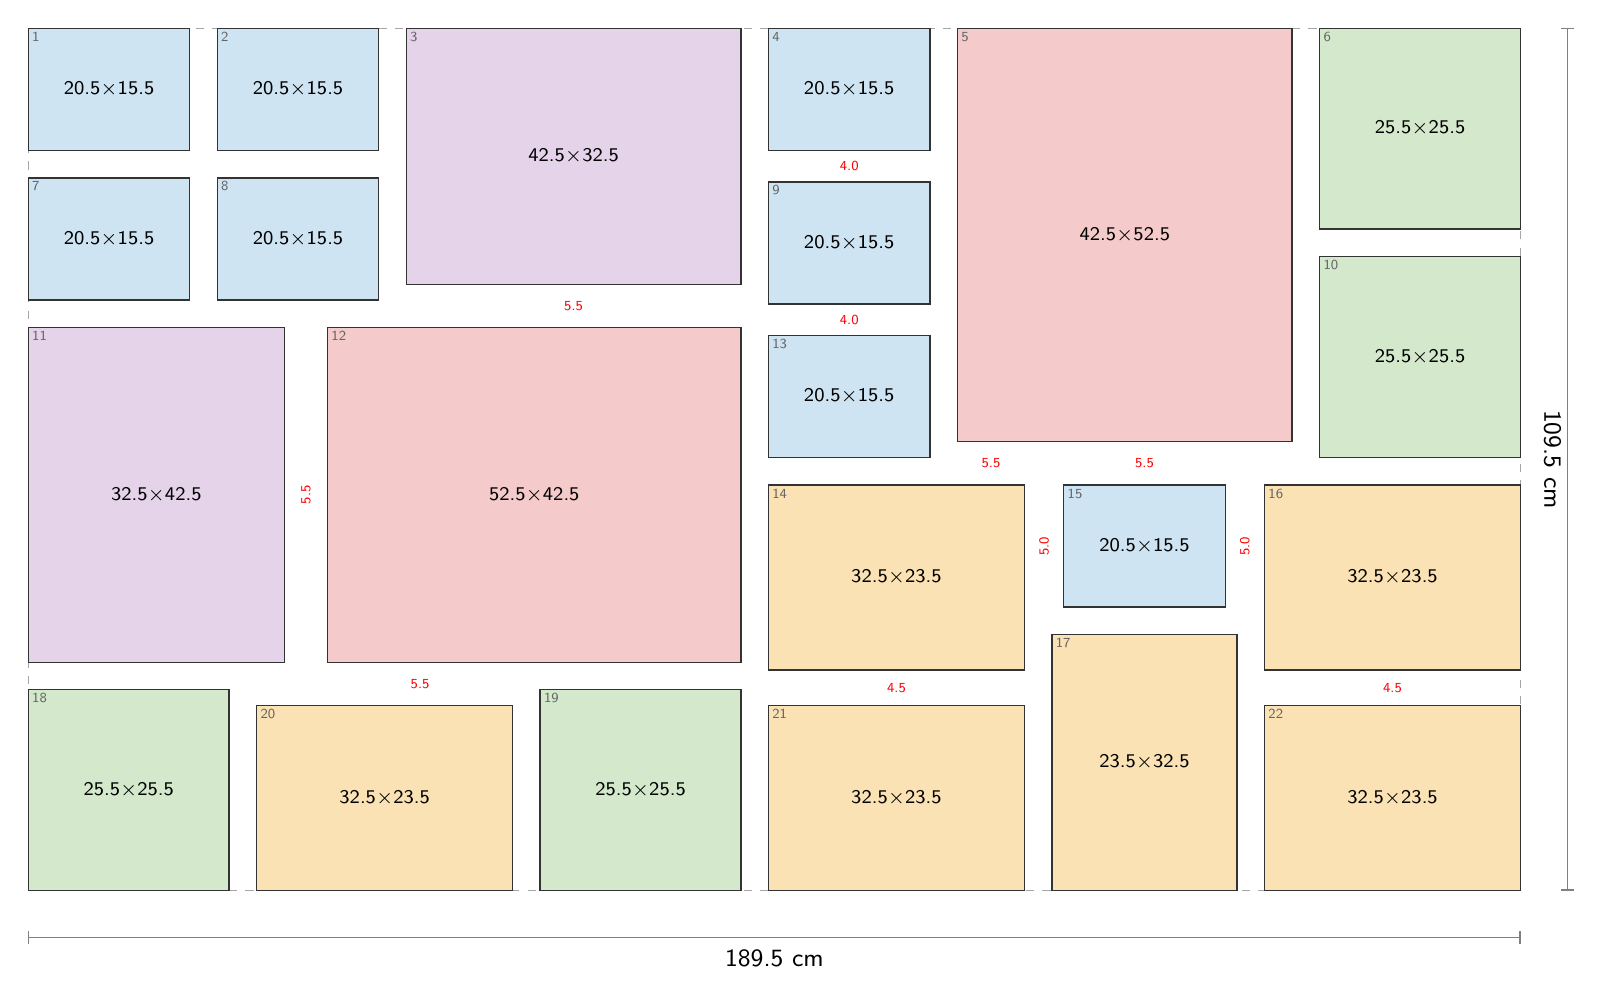
\begin{tikzpicture}[x=1mm, y=-1mm]
\draw[gray!70, dashed, line width=0.4pt] (0,0) rectangle (189.50,109.50);
\filldraw[fill=ft0, draw=black!80, line width=0.5pt] (0.00,0.00) rectangle (20.50,15.50);
\node[align=center, inner sep=0pt] at (10.25,7.75) {\scriptsize 20.5$\times$15.5};
\node[anchor=north west, inner sep=1.2pt, font=\tiny, text=black!60] at (0.00,0.00) {1};
\filldraw[fill=ft0, draw=black!80, line width=0.5pt] (24.00,0.00) rectangle (44.50,15.50);
\node[align=center, inner sep=0pt] at (34.25,7.75) {\scriptsize 20.5$\times$15.5};
\node[anchor=north west, inner sep=1.2pt, font=\tiny, text=black!60] at (24.00,0.00) {2};
\filldraw[fill=ft3, draw=black!80, line width=0.5pt] (48.00,0.00) rectangle (90.50,32.50);
\node[align=center, inner sep=0pt] at (69.25,16.25) {\scriptsize 42.5$\times$32.5};
\node[anchor=north west, inner sep=1.2pt, font=\tiny, text=black!60] at (48.00,0.00) {3};
\filldraw[fill=ft0, draw=black!80, line width=0.5pt] (94.00,0.00) rectangle (114.50,15.50);
\node[align=center, inner sep=0pt] at (104.25,7.75) {\scriptsize 20.5$\times$15.5};
\node[anchor=north west, inner sep=1.2pt, font=\tiny, text=black!60] at (94.00,0.00) {4};
\filldraw[fill=ft4, draw=black!80, line width=0.5pt] (118.00,0.00) rectangle (160.50,52.50);
\node[align=center, inner sep=0pt] at (139.25,26.25) {\scriptsize 42.5$\times$52.5};
\node[anchor=north west, inner sep=1.2pt, font=\tiny, text=black!60] at (118.00,0.00) {5};
\filldraw[fill=ft2, draw=black!80, line width=0.5pt] (164.00,0.00) rectangle (189.50,25.50);
\node[align=center, inner sep=0pt] at (176.75,12.75) {\scriptsize 25.5$\times$25.5};
\node[anchor=north west, inner sep=1.2pt, font=\tiny, text=black!60] at (164.00,0.00) {6};
\filldraw[fill=ft0, draw=black!80, line width=0.5pt] (0.00,19.00) rectangle (20.50,34.50);
\node[align=center, inner sep=0pt] at (10.25,26.75) {\scriptsize 20.5$\times$15.5};
\node[anchor=north west, inner sep=1.2pt, font=\tiny, text=black!60] at (0.00,19.00) {7};
\filldraw[fill=ft0, draw=black!80, line width=0.5pt] (24.00,19.00) rectangle (44.50,34.50);
\node[align=center, inner sep=0pt] at (34.25,26.75) {\scriptsize 20.5$\times$15.5};
\node[anchor=north west, inner sep=1.2pt, font=\tiny, text=black!60] at (24.00,19.00) {8};
\filldraw[fill=ft0, draw=black!80, line width=0.5pt] (94.00,19.50) rectangle (114.50,35.00);
\node[align=center, inner sep=0pt] at (104.25,27.25) {\scriptsize 20.5$\times$15.5};
\node[anchor=north west, inner sep=1.2pt, font=\tiny, text=black!60] at (94.00,19.50) {9};
\filldraw[fill=ft2, draw=black!80, line width=0.5pt] (164.00,29.00) rectangle (189.50,54.50);
\node[align=center, inner sep=0pt] at (176.75,41.75) {\scriptsize 25.5$\times$25.5};
\node[anchor=north west, inner sep=1.2pt, font=\tiny, text=black!60] at (164.00,29.00) {10};
\filldraw[fill=ft3, draw=black!80, line width=0.5pt] (0.00,38.00) rectangle (32.50,80.50);
\node[align=center, inner sep=0pt] at (16.25,59.25) {\scriptsize 32.5$\times$42.5};
\node[anchor=north west, inner sep=1.2pt, font=\tiny, text=black!60] at (0.00,38.00) {11};
\filldraw[fill=ft4, draw=black!80, line width=0.5pt] (38.00,38.00) rectangle (90.50,80.50);
\node[align=center, inner sep=0pt] at (64.25,59.25) {\scriptsize 52.5$\times$42.5};
\node[anchor=north west, inner sep=1.2pt, font=\tiny, text=black!60] at (38.00,38.00) {12};
\filldraw[fill=ft0, draw=black!80, line width=0.5pt] (94.00,39.00) rectangle (114.50,54.50);
\node[align=center, inner sep=0pt] at (104.25,46.75) {\scriptsize 20.5$\times$15.5};
\node[anchor=north west, inner sep=1.2pt, font=\tiny, text=black!60] at (94.00,39.00) {13};
\filldraw[fill=ft1, draw=black!80, line width=0.5pt] (94.00,58.00) rectangle (126.50,81.50);
\node[align=center, inner sep=0pt] at (110.25,69.75) {\scriptsize 32.5$\times$23.5};
\node[anchor=north west, inner sep=1.2pt, font=\tiny, text=black!60] at (94.00,58.00) {14};
\filldraw[fill=ft0, draw=black!80, line width=0.5pt] (131.50,58.00) rectangle (152.00,73.50);
\node[align=center, inner sep=0pt] at (141.75,65.75) {\scriptsize 20.5$\times$15.5};
\node[anchor=north west, inner sep=1.2pt, font=\tiny, text=black!60] at (131.50,58.00) {15};
\filldraw[fill=ft1, draw=black!80, line width=0.5pt] (157.00,58.00) rectangle (189.50,81.50);
\node[align=center, inner sep=0pt] at (173.25,69.75) {\scriptsize 32.5$\times$23.5};
\node[anchor=north west, inner sep=1.2pt, font=\tiny, text=black!60] at (157.00,58.00) {16};
\filldraw[fill=ft1, draw=black!80, line width=0.5pt] (130.00,77.00) rectangle (153.50,109.50);
\node[align=center, inner sep=0pt] at (141.75,93.25) {\scriptsize 23.5$\times$32.5};
\node[anchor=north west, inner sep=1.2pt, font=\tiny, text=black!60] at (130.00,77.00) {17};
\filldraw[fill=ft2, draw=black!80, line width=0.5pt] (0.00,84.00) rectangle (25.50,109.50);
\node[align=center, inner sep=0pt] at (12.75,96.75) {\scriptsize 25.5$\times$25.5};
\node[anchor=north west, inner sep=1.2pt, font=\tiny, text=black!60] at (0.00,84.00) {18};
\filldraw[fill=ft2, draw=black!80, line width=0.5pt] (65.00,84.00) rectangle (90.50,109.50);
\node[align=center, inner sep=0pt] at (77.75,96.75) {\scriptsize 25.5$\times$25.5};
\node[anchor=north west, inner sep=1.2pt, font=\tiny, text=black!60] at (65.00,84.00) {19};
\filldraw[fill=ft1, draw=black!80, line width=0.5pt] (29.00,86.00) rectangle (61.50,109.50);
\node[align=center, inner sep=0pt] at (45.25,97.75) {\scriptsize 32.5$\times$23.5};
\node[anchor=north west, inner sep=1.2pt, font=\tiny, text=black!60] at (29.00,86.00) {20};
\filldraw[fill=ft1, draw=black!80, line width=0.5pt] (94.00,86.00) rectangle (126.50,109.50);
\node[align=center, inner sep=0pt] at (110.25,97.75) {\scriptsize 32.5$\times$23.5};
\node[anchor=north west, inner sep=1.2pt, font=\tiny, text=black!60] at (94.00,86.00) {21};
\filldraw[fill=ft1, draw=black!80, line width=0.5pt] (157.00,86.00) rectangle (189.50,109.50);
\node[align=center, inner sep=0pt] at (173.25,97.75) {\scriptsize 32.5$\times$23.5};
\node[anchor=north west, inner sep=1.2pt, font=\tiny, text=black!60] at (157.00,86.00) {22};
\node[font=\tiny, text=red, fill=white, inner sep=0.3pt] at (69.25,35.25) {5.5};
\node[font=\tiny, text=red, fill=white, inner sep=0.3pt] at (104.25,17.50) {4.0};
\node[font=\tiny, text=red, fill=white, inner sep=0.3pt] at (122.25,55.25) {5.5};
\node[font=\tiny, text=red, fill=white, inner sep=0.3pt] at (141.75,55.25) {5.5};
\node[font=\tiny, text=red, fill=white, inner sep=0.3pt] at (104.25,37.00) {4.0};
\node[font=\tiny, text=red, fill=white, inner sep=0.3pt, rotate=90] at (35.25,59.25) {5.5};
\node[font=\tiny, text=red, fill=white, inner sep=0.3pt] at (49.75,83.25) {5.5};
\node[font=\tiny, text=red, fill=white, inner sep=0.3pt, rotate=90] at (129.00,65.75) {5.0};
\node[font=\tiny, text=red, fill=white, inner sep=0.3pt] at (110.25,83.75) {4.5};
\node[font=\tiny, text=red, fill=white, inner sep=0.3pt, rotate=90] at (154.50,65.75) {5.0};
\node[font=\tiny, text=red, fill=white, inner sep=0.3pt] at (173.25,83.75) {4.5};
\draw[Bar-Bar, gray] (0,115.50) -- (189.50,115.50) node[midway, below=1pt, font=\small, text=black] {189.5 cm};
\draw[Bar-Bar, gray] (195.50,0) -- (195.50,109.50) node[midway, right=1pt, font=\small, text=black, rotate=-90, anchor=north] {109.5 cm};
\end{tikzpicture}\\[4pt]
{\scriptsize Scale 1:10 (1 mm = 1 cm). Red numbers mark gaps that deviate from the nominal gap by more than 0.25 cm. Small grey numbers index the coordinate table.}
\end{minipage}\hfill
\begin{minipage}[t]{0.25\textwidth}\vspace{0pt}
\small
\begin{tabular}{@{}l l@{}}
\toprule
Outer size & 189.5 $\times$ 109.5 cm \\
Nominal gap & 3.5 cm \\
Actual gaps & 3.5 -- 5.5 cm \\
Max.\ deviation & 2.0 cm \\
Mean deviation & 0.40 cm \\
Border notches & none \\
Corners filled & 4 / 4 \\
Frames used & 22 of 28 \\
\bottomrule
\end{tabular}

\vspace{8pt}
\scriptsize
\begin{tabular}{@{}c l l r r@{}}
\toprule
 & outer w $\times$ h (cm) & & used & have \\
\midrule
\tikz[baseline=-0.6ex]\fill[ft0,draw=black!60] (0,0) rectangle (1.2ex,1.2ex); & 20.5$\times$15.5 & L & 8 & 9 \\
\tikz[baseline=-0.6ex]\fill[ft0,draw=black!60] (0,0) rectangle (1.2ex,1.2ex); & 15.5$\times$20.5 & P & 0 & 2 \\
\tikz[baseline=-0.6ex]\fill[ft3,draw=black!60] (0,0) rectangle (1.2ex,1.2ex); & 32.5$\times$42.5 & P & 1 & 2 \\
\tikz[baseline=-0.6ex]\fill[ft3,draw=black!60] (0,0) rectangle (1.2ex,1.2ex); & 42.5$\times$32.5 & L & 1 & 1 \\
\tikz[baseline=-0.6ex]\fill[ft1,draw=black!60] (0,0) rectangle (1.2ex,1.2ex); & 32.5$\times$23.5 & L & 5 & 5 \\
\tikz[baseline=-0.6ex]\fill[ft1,draw=black!60] (0,0) rectangle (1.2ex,1.2ex); & 23.5$\times$32.5 & P & 1 & 1 \\
\tikz[baseline=-0.6ex]\fill[ft2,draw=black!60] (0,0) rectangle (1.2ex,1.2ex); & 25.5$\times$25.5 &  & 4 & 5 \\
\tikz[baseline=-0.6ex]\fill[ft4,draw=black!60] (0,0) rectangle (1.2ex,1.2ex); & 42.5$\times$52.5 & P & 1 & 1 \\
\tikz[baseline=-0.6ex]\fill[ft4,draw=black!60] (0,0) rectangle (1.2ex,1.2ex); & 52.5$\times$42.5 & L & 1 & 2 \\
\bottomrule
\end{tabular}

\vspace{8pt}
{\bfseries Positions} (top-left corner, cm)\\[2pt]
\tiny
\begin{tabular}{@{}r l r r@{}}
\toprule
\# & frame w $\times$ h & x & y \\
\midrule
1 & 20.5 $\times$ 15.5 & 0.0 & 0.0 \\
2 & 20.5 $\times$ 15.5 & 24.0 & 0.0 \\
3 & 42.5 $\times$ 32.5 & 48.0 & 0.0 \\
4 & 20.5 $\times$ 15.5 & 94.0 & 0.0 \\
5 & 42.5 $\times$ 52.5 & 118.0 & 0.0 \\
6 & 25.5 $\times$ 25.5 & 164.0 & 0.0 \\
7 & 20.5 $\times$ 15.5 & 0.0 & 19.0 \\
8 & 20.5 $\times$ 15.5 & 24.0 & 19.0 \\
9 & 20.5 $\times$ 15.5 & 94.0 & 19.5 \\
10 & 25.5 $\times$ 25.5 & 164.0 & 29.0 \\
11 & 32.5 $\times$ 42.5 & 0.0 & 38.0 \\
12 & 52.5 $\times$ 42.5 & 38.0 & 38.0 \\
13 & 20.5 $\times$ 15.5 & 94.0 & 39.0 \\
14 & 32.5 $\times$ 23.5 & 94.0 & 58.0 \\
15 & 20.5 $\times$ 15.5 & 131.5 & 58.0 \\
16 & 32.5 $\times$ 23.5 & 157.0 & 58.0 \\
17 & 23.5 $\times$ 32.5 & 130.0 & 77.0 \\
18 & 25.5 $\times$ 25.5 & 0.0 & 84.0 \\
19 & 25.5 $\times$ 25.5 & 65.0 & 84.0 \\
20 & 32.5 $\times$ 23.5 & 29.0 & 86.0 \\
21 & 32.5 $\times$ 23.5 & 94.0 & 86.0 \\
22 & 32.5 $\times$ 23.5 & 157.0 & 86.0 \\
\bottomrule
\end{tabular}
\end{minipage}
\clearpage

\begin{minipage}[t]{0.74\textwidth}\vspace{0pt}
{\LARGE\bfseries Layout 5}\hspace{1.5em}{\large 181.5 $\times$ 113.5 cm \quad gap 1.5 cm \quad 20 frames}\\[8pt]
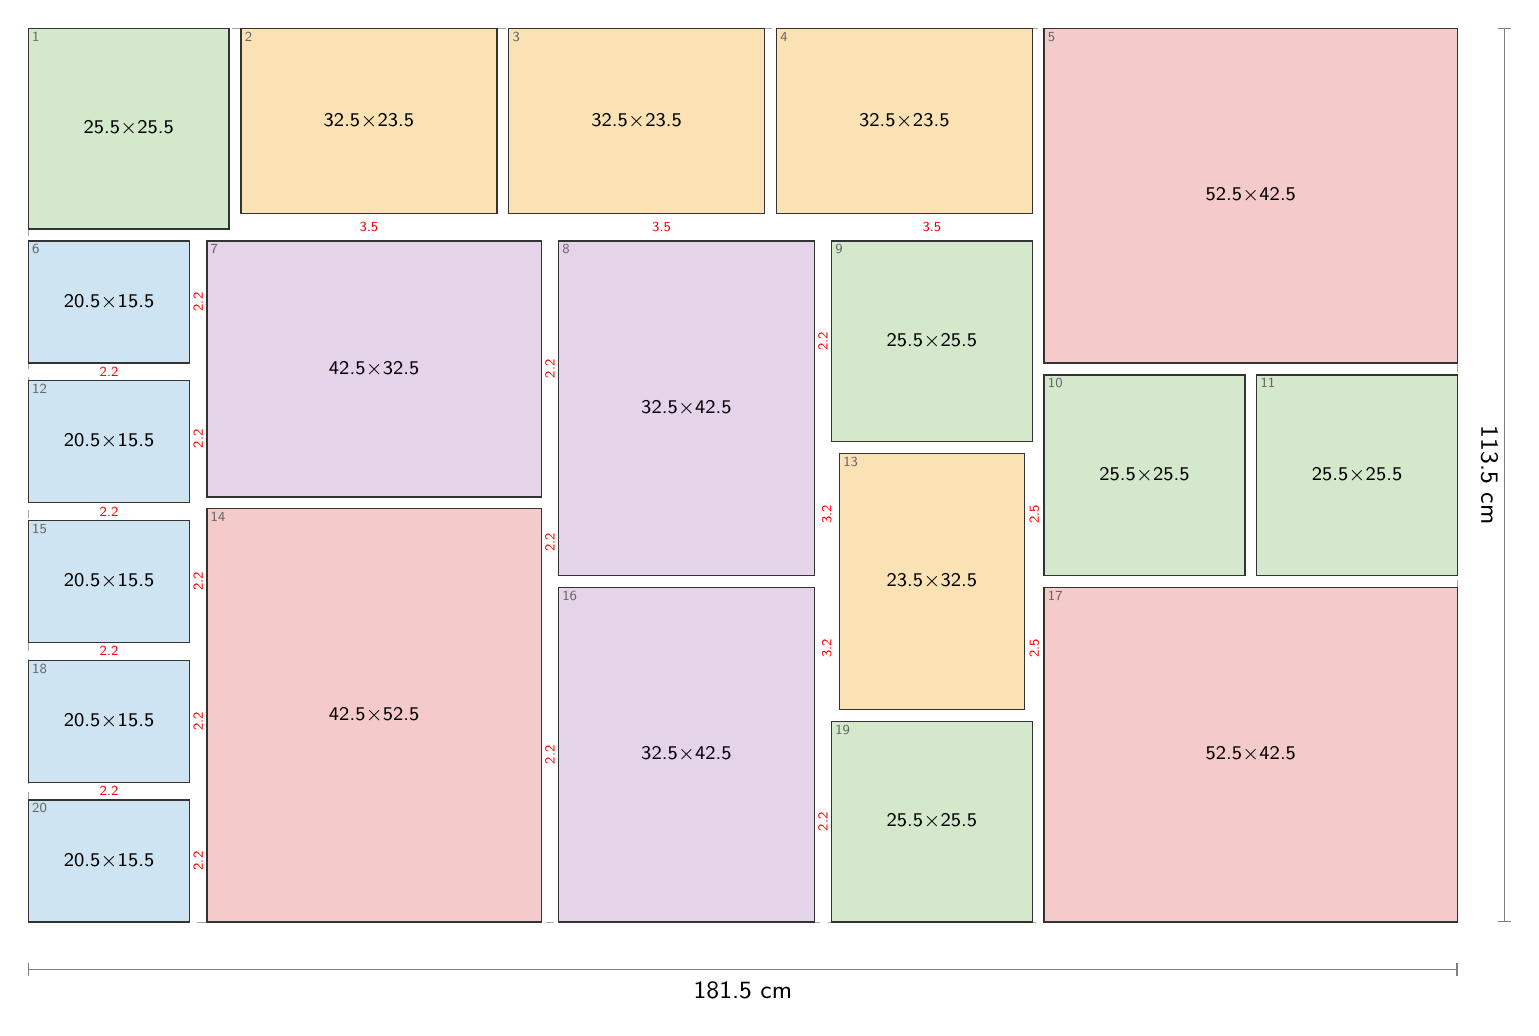
\begin{tikzpicture}[x=1mm, y=-1mm]
\draw[gray!70, dashed, line width=0.4pt] (0,0) rectangle (181.50,113.50);
\filldraw[fill=ft2, draw=black!80, line width=0.5pt] (0.00,0.00) rectangle (25.50,25.50);
\node[align=center, inner sep=0pt] at (12.75,12.75) {\scriptsize 25.5$\times$25.5};
\node[anchor=north west, inner sep=1.2pt, font=\tiny, text=black!60] at (0.00,0.00) {1};
\filldraw[fill=ft1, draw=black!80, line width=0.5pt] (27.00,0.00) rectangle (59.50,23.50);
\node[align=center, inner sep=0pt] at (43.25,11.75) {\scriptsize 32.5$\times$23.5};
\node[anchor=north west, inner sep=1.2pt, font=\tiny, text=black!60] at (27.00,0.00) {2};
\filldraw[fill=ft1, draw=black!80, line width=0.5pt] (61.00,0.00) rectangle (93.50,23.50);
\node[align=center, inner sep=0pt] at (77.25,11.75) {\scriptsize 32.5$\times$23.5};
\node[anchor=north west, inner sep=1.2pt, font=\tiny, text=black!60] at (61.00,0.00) {3};
\filldraw[fill=ft1, draw=black!80, line width=0.5pt] (95.00,0.00) rectangle (127.50,23.50);
\node[align=center, inner sep=0pt] at (111.25,11.75) {\scriptsize 32.5$\times$23.5};
\node[anchor=north west, inner sep=1.2pt, font=\tiny, text=black!60] at (95.00,0.00) {4};
\filldraw[fill=ft4, draw=black!80, line width=0.5pt] (129.00,0.00) rectangle (181.50,42.50);
\node[align=center, inner sep=0pt] at (155.25,21.25) {\scriptsize 52.5$\times$42.5};
\node[anchor=north west, inner sep=1.2pt, font=\tiny, text=black!60] at (129.00,0.00) {5};
\filldraw[fill=ft0, draw=black!80, line width=0.5pt] (0.00,27.00) rectangle (20.50,42.50);
\node[align=center, inner sep=0pt] at (10.25,34.75) {\scriptsize 20.5$\times$15.5};
\node[anchor=north west, inner sep=1.2pt, font=\tiny, text=black!60] at (0.00,27.00) {6};
\filldraw[fill=ft3, draw=black!80, line width=0.5pt] (22.67,27.00) rectangle (65.17,59.50);
\node[align=center, inner sep=0pt] at (43.92,43.25) {\scriptsize 42.5$\times$32.5};
\node[anchor=north west, inner sep=1.2pt, font=\tiny, text=black!60] at (22.67,27.00) {7};
\filldraw[fill=ft3, draw=black!80, line width=0.5pt] (67.33,27.00) rectangle (99.83,69.50);
\node[align=center, inner sep=0pt] at (83.58,48.25) {\scriptsize 32.5$\times$42.5};
\node[anchor=north west, inner sep=1.2pt, font=\tiny, text=black!60] at (67.33,27.00) {8};
\filldraw[fill=ft2, draw=black!80, line width=0.5pt] (102.00,27.00) rectangle (127.50,52.50);
\node[align=center, inner sep=0pt] at (114.75,39.75) {\scriptsize 25.5$\times$25.5};
\node[anchor=north west, inner sep=1.2pt, font=\tiny, text=black!60] at (102.00,27.00) {9};
\filldraw[fill=ft2, draw=black!80, line width=0.5pt] (129.00,44.00) rectangle (154.50,69.50);
\node[align=center, inner sep=0pt] at (141.75,56.75) {\scriptsize 25.5$\times$25.5};
\node[anchor=north west, inner sep=1.2pt, font=\tiny, text=black!60] at (129.00,44.00) {10};
\filldraw[fill=ft2, draw=black!80, line width=0.5pt] (156.00,44.00) rectangle (181.50,69.50);
\node[align=center, inner sep=0pt] at (168.75,56.75) {\scriptsize 25.5$\times$25.5};
\node[anchor=north west, inner sep=1.2pt, font=\tiny, text=black!60] at (156.00,44.00) {11};
\filldraw[fill=ft0, draw=black!80, line width=0.5pt] (0.00,44.75) rectangle (20.50,60.25);
\node[align=center, inner sep=0pt] at (10.25,52.50) {\scriptsize 20.5$\times$15.5};
\node[anchor=north west, inner sep=1.2pt, font=\tiny, text=black!60] at (0.00,44.75) {12};
\filldraw[fill=ft1, draw=black!80, line width=0.5pt] (103.00,54.00) rectangle (126.50,86.50);
\node[align=center, inner sep=0pt] at (114.75,70.25) {\scriptsize 23.5$\times$32.5};
\node[anchor=north west, inner sep=1.2pt, font=\tiny, text=black!60] at (103.00,54.00) {13};
\filldraw[fill=ft4, draw=black!80, line width=0.5pt] (22.67,61.00) rectangle (65.17,113.50);
\node[align=center, inner sep=0pt] at (43.92,87.25) {\scriptsize 42.5$\times$52.5};
\node[anchor=north west, inner sep=1.2pt, font=\tiny, text=black!60] at (22.67,61.00) {14};
\filldraw[fill=ft0, draw=black!80, line width=0.5pt] (0.00,62.50) rectangle (20.50,78.00);
\node[align=center, inner sep=0pt] at (10.25,70.25) {\scriptsize 20.5$\times$15.5};
\node[anchor=north west, inner sep=1.2pt, font=\tiny, text=black!60] at (0.00,62.50) {15};
\filldraw[fill=ft3, draw=black!80, line width=0.5pt] (67.33,71.00) rectangle (99.83,113.50);
\node[align=center, inner sep=0pt] at (83.58,92.25) {\scriptsize 32.5$\times$42.5};
\node[anchor=north west, inner sep=1.2pt, font=\tiny, text=black!60] at (67.33,71.00) {16};
\filldraw[fill=ft4, draw=black!80, line width=0.5pt] (129.00,71.00) rectangle (181.50,113.50);
\node[align=center, inner sep=0pt] at (155.25,92.25) {\scriptsize 52.5$\times$42.5};
\node[anchor=north west, inner sep=1.2pt, font=\tiny, text=black!60] at (129.00,71.00) {17};
\filldraw[fill=ft0, draw=black!80, line width=0.5pt] (0.00,80.25) rectangle (20.50,95.75);
\node[align=center, inner sep=0pt] at (10.25,88.00) {\scriptsize 20.5$\times$15.5};
\node[anchor=north west, inner sep=1.2pt, font=\tiny, text=black!60] at (0.00,80.25) {18};
\filldraw[fill=ft2, draw=black!80, line width=0.5pt] (102.00,88.00) rectangle (127.50,113.50);
\node[align=center, inner sep=0pt] at (114.75,100.75) {\scriptsize 25.5$\times$25.5};
\node[anchor=north west, inner sep=1.2pt, font=\tiny, text=black!60] at (102.00,88.00) {19};
\filldraw[fill=ft0, draw=black!80, line width=0.5pt] (0.00,98.00) rectangle (20.50,113.50);
\node[align=center, inner sep=0pt] at (10.25,105.75) {\scriptsize 20.5$\times$15.5};
\node[anchor=north west, inner sep=1.2pt, font=\tiny, text=black!60] at (0.00,98.00) {20};
\node[font=\tiny, text=red, fill=white, inner sep=0.3pt] at (43.25,25.25) {3.5};
\node[font=\tiny, text=red, fill=white, inner sep=0.3pt] at (80.42,25.25) {3.5};
\node[font=\tiny, text=red, fill=white, inner sep=0.3pt] at (114.75,25.25) {3.5};
\node[font=\tiny, text=red, fill=white, inner sep=0.3pt, rotate=90] at (21.58,34.75) {2.2};
\node[font=\tiny, text=red, fill=white, inner sep=0.3pt] at (10.25,43.62) {2.2};
\node[font=\tiny, text=red, fill=white, inner sep=0.3pt, rotate=90] at (66.25,43.25) {2.2};
\node[font=\tiny, text=red, fill=white, inner sep=0.3pt, rotate=90] at (100.92,39.75) {2.2};
\node[font=\tiny, text=red, fill=white, inner sep=0.3pt, rotate=90] at (101.42,61.75) {3.2};
\node[font=\tiny, text=red, fill=white, inner sep=0.3pt, rotate=90] at (21.58,52.12) {2.2};
\node[font=\tiny, text=red, fill=white, inner sep=0.3pt] at (10.25,61.38) {2.2};
\node[font=\tiny, text=red, fill=white, inner sep=0.3pt, rotate=90] at (127.75,61.75) {2.5};
\node[font=\tiny, text=red, fill=white, inner sep=0.3pt, rotate=90] at (127.75,78.75) {2.5};
\node[font=\tiny, text=red, fill=white, inner sep=0.3pt, rotate=90] at (66.25,65.25) {2.2};
\node[font=\tiny, text=red, fill=white, inner sep=0.3pt, rotate=90] at (66.25,92.25) {2.2};
\node[font=\tiny, text=red, fill=white, inner sep=0.3pt, rotate=90] at (21.58,70.25) {2.2};
\node[font=\tiny, text=red, fill=white, inner sep=0.3pt] at (10.25,79.12) {2.2};
\node[font=\tiny, text=red, fill=white, inner sep=0.3pt, rotate=90] at (101.42,78.75) {3.2};
\node[font=\tiny, text=red, fill=white, inner sep=0.3pt, rotate=90] at (100.92,100.75) {2.2};
\node[font=\tiny, text=red, fill=white, inner sep=0.3pt, rotate=90] at (21.58,88.00) {2.2};
\node[font=\tiny, text=red, fill=white, inner sep=0.3pt] at (10.25,96.88) {2.2};
\node[font=\tiny, text=red, fill=white, inner sep=0.3pt, rotate=90] at (21.58,105.75) {2.2};
\draw[Bar-Bar, gray] (0,119.50) -- (181.50,119.50) node[midway, below=1pt, font=\small, text=black] {181.5 cm};
\draw[Bar-Bar, gray] (187.50,0) -- (187.50,113.50) node[midway, right=1pt, font=\small, text=black, rotate=-90, anchor=north] {113.5 cm};
\end{tikzpicture}\\[4pt]
{\scriptsize Scale 1:10 (1 mm = 1 cm). Red numbers mark gaps that deviate from the nominal gap by more than 0.25 cm. Small grey numbers index the coordinate table.}
\end{minipage}\hfill
\begin{minipage}[t]{0.25\textwidth}\vspace{0pt}
\small
\begin{tabular}{@{}l l@{}}
\toprule
Outer size & 181.5 $\times$ 113.5 cm \\
Nominal gap & 1.5 cm \\
Actual gaps & 1.5 -- 3.5 cm \\
Max.\ deviation & 2.0 cm \\
Mean deviation & 0.55 cm \\
Border notches & none \\
Corners filled & 4 / 4 \\
Frames used & 20 of 28 \\
\bottomrule
\end{tabular}

\vspace{8pt}
\scriptsize
\begin{tabular}{@{}c l l r r@{}}
\toprule
 & outer w $\times$ h (cm) & & used & have \\
\midrule
\tikz[baseline=-0.6ex]\fill[ft0,draw=black!60] (0,0) rectangle (1.2ex,1.2ex); & 20.5$\times$15.5 & L & 5 & 9 \\
\tikz[baseline=-0.6ex]\fill[ft0,draw=black!60] (0,0) rectangle (1.2ex,1.2ex); & 15.5$\times$20.5 & P & 0 & 2 \\
\tikz[baseline=-0.6ex]\fill[ft3,draw=black!60] (0,0) rectangle (1.2ex,1.2ex); & 32.5$\times$42.5 & P & 2 & 2 \\
\tikz[baseline=-0.6ex]\fill[ft3,draw=black!60] (0,0) rectangle (1.2ex,1.2ex); & 42.5$\times$32.5 & L & 1 & 1 \\
\tikz[baseline=-0.6ex]\fill[ft1,draw=black!60] (0,0) rectangle (1.2ex,1.2ex); & 32.5$\times$23.5 & L & 3 & 5 \\
\tikz[baseline=-0.6ex]\fill[ft1,draw=black!60] (0,0) rectangle (1.2ex,1.2ex); & 23.5$\times$32.5 & P & 1 & 1 \\
\tikz[baseline=-0.6ex]\fill[ft2,draw=black!60] (0,0) rectangle (1.2ex,1.2ex); & 25.5$\times$25.5 &  & 5 & 5 \\
\tikz[baseline=-0.6ex]\fill[ft4,draw=black!60] (0,0) rectangle (1.2ex,1.2ex); & 42.5$\times$52.5 & P & 1 & 1 \\
\tikz[baseline=-0.6ex]\fill[ft4,draw=black!60] (0,0) rectangle (1.2ex,1.2ex); & 52.5$\times$42.5 & L & 2 & 2 \\
\bottomrule
\end{tabular}

\vspace{8pt}
{\bfseries Positions} (top-left corner, cm)\\[2pt]
\tiny
\begin{tabular}{@{}r l r r@{}}
\toprule
\# & frame w $\times$ h & x & y \\
\midrule
1 & 25.5 $\times$ 25.5 & 0.0 & 0.0 \\
2 & 32.5 $\times$ 23.5 & 27.0 & 0.0 \\
3 & 32.5 $\times$ 23.5 & 61.0 & 0.0 \\
4 & 32.5 $\times$ 23.5 & 95.0 & 0.0 \\
5 & 52.5 $\times$ 42.5 & 129.0 & 0.0 \\
6 & 20.5 $\times$ 15.5 & 0.0 & 27.0 \\
7 & 42.5 $\times$ 32.5 & 22.7 & 27.0 \\
8 & 32.5 $\times$ 42.5 & 67.3 & 27.0 \\
9 & 25.5 $\times$ 25.5 & 102.0 & 27.0 \\
10 & 25.5 $\times$ 25.5 & 129.0 & 44.0 \\
11 & 25.5 $\times$ 25.5 & 156.0 & 44.0 \\
12 & 20.5 $\times$ 15.5 & 0.0 & 44.8 \\
13 & 23.5 $\times$ 32.5 & 103.0 & 54.0 \\
14 & 42.5 $\times$ 52.5 & 22.7 & 61.0 \\
15 & 20.5 $\times$ 15.5 & 0.0 & 62.5 \\
16 & 32.5 $\times$ 42.5 & 67.3 & 71.0 \\
17 & 52.5 $\times$ 42.5 & 129.0 & 71.0 \\
18 & 20.5 $\times$ 15.5 & 0.0 & 80.2 \\
19 & 25.5 $\times$ 25.5 & 102.0 & 88.0 \\
20 & 20.5 $\times$ 15.5 & 0.0 & 98.0 \\
\bottomrule
\end{tabular}
\end{minipage}
\clearpage

\begin{minipage}[t]{0.74\textwidth}\vspace{0pt}
{\LARGE\bfseries Layout 6}\hspace{1.5em}{\large 181.5 $\times$ 113.5 cm \quad gap 1.5 cm \quad 20 frames}\\[8pt]
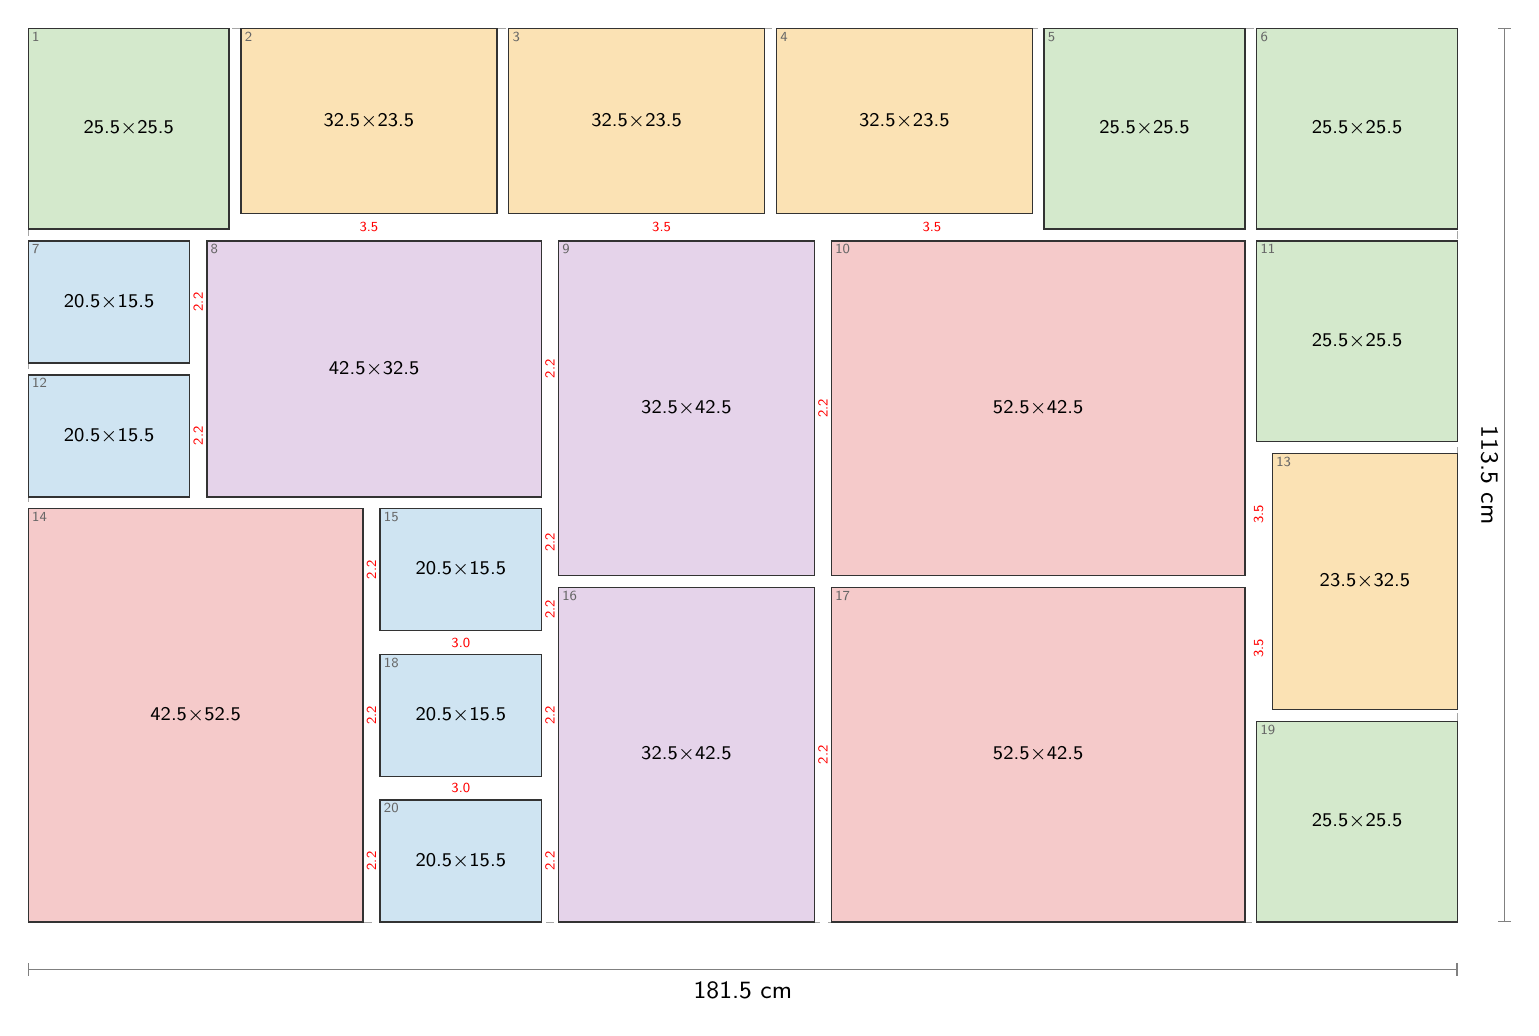
\begin{tikzpicture}[x=1mm, y=-1mm]
\draw[gray!70, dashed, line width=0.4pt] (0,0) rectangle (181.50,113.50);
\filldraw[fill=ft2, draw=black!80, line width=0.5pt] (0.00,0.00) rectangle (25.50,25.50);
\node[align=center, inner sep=0pt] at (12.75,12.75) {\scriptsize 25.5$\times$25.5};
\node[anchor=north west, inner sep=1.2pt, font=\tiny, text=black!60] at (0.00,0.00) {1};
\filldraw[fill=ft1, draw=black!80, line width=0.5pt] (27.00,0.00) rectangle (59.50,23.50);
\node[align=center, inner sep=0pt] at (43.25,11.75) {\scriptsize 32.5$\times$23.5};
\node[anchor=north west, inner sep=1.2pt, font=\tiny, text=black!60] at (27.00,0.00) {2};
\filldraw[fill=ft1, draw=black!80, line width=0.5pt] (61.00,0.00) rectangle (93.50,23.50);
\node[align=center, inner sep=0pt] at (77.25,11.75) {\scriptsize 32.5$\times$23.5};
\node[anchor=north west, inner sep=1.2pt, font=\tiny, text=black!60] at (61.00,0.00) {3};
\filldraw[fill=ft1, draw=black!80, line width=0.5pt] (95.00,0.00) rectangle (127.50,23.50);
\node[align=center, inner sep=0pt] at (111.25,11.75) {\scriptsize 32.5$\times$23.5};
\node[anchor=north west, inner sep=1.2pt, font=\tiny, text=black!60] at (95.00,0.00) {4};
\filldraw[fill=ft2, draw=black!80, line width=0.5pt] (129.00,0.00) rectangle (154.50,25.50);
\node[align=center, inner sep=0pt] at (141.75,12.75) {\scriptsize 25.5$\times$25.5};
\node[anchor=north west, inner sep=1.2pt, font=\tiny, text=black!60] at (129.00,0.00) {5};
\filldraw[fill=ft2, draw=black!80, line width=0.5pt] (156.00,0.00) rectangle (181.50,25.50);
\node[align=center, inner sep=0pt] at (168.75,12.75) {\scriptsize 25.5$\times$25.5};
\node[anchor=north west, inner sep=1.2pt, font=\tiny, text=black!60] at (156.00,0.00) {6};
\filldraw[fill=ft0, draw=black!80, line width=0.5pt] (0.00,27.00) rectangle (20.50,42.50);
\node[align=center, inner sep=0pt] at (10.25,34.75) {\scriptsize 20.5$\times$15.5};
\node[anchor=north west, inner sep=1.2pt, font=\tiny, text=black!60] at (0.00,27.00) {7};
\filldraw[fill=ft3, draw=black!80, line width=0.5pt] (22.67,27.00) rectangle (65.17,59.50);
\node[align=center, inner sep=0pt] at (43.92,43.25) {\scriptsize 42.5$\times$32.5};
\node[anchor=north west, inner sep=1.2pt, font=\tiny, text=black!60] at (22.67,27.00) {8};
\filldraw[fill=ft3, draw=black!80, line width=0.5pt] (67.33,27.00) rectangle (99.83,69.50);
\node[align=center, inner sep=0pt] at (83.58,48.25) {\scriptsize 32.5$\times$42.5};
\node[anchor=north west, inner sep=1.2pt, font=\tiny, text=black!60] at (67.33,27.00) {9};
\filldraw[fill=ft4, draw=black!80, line width=0.5pt] (102.00,27.00) rectangle (154.50,69.50);
\node[align=center, inner sep=0pt] at (128.25,48.25) {\scriptsize 52.5$\times$42.5};
\node[anchor=north west, inner sep=1.2pt, font=\tiny, text=black!60] at (102.00,27.00) {10};
\filldraw[fill=ft2, draw=black!80, line width=0.5pt] (156.00,27.00) rectangle (181.50,52.50);
\node[align=center, inner sep=0pt] at (168.75,39.75) {\scriptsize 25.5$\times$25.5};
\node[anchor=north west, inner sep=1.2pt, font=\tiny, text=black!60] at (156.00,27.00) {11};
\filldraw[fill=ft0, draw=black!80, line width=0.5pt] (0.00,44.00) rectangle (20.50,59.50);
\node[align=center, inner sep=0pt] at (10.25,51.75) {\scriptsize 20.5$\times$15.5};
\node[anchor=north west, inner sep=1.2pt, font=\tiny, text=black!60] at (0.00,44.00) {12};
\filldraw[fill=ft1, draw=black!80, line width=0.5pt] (158.00,54.00) rectangle (181.50,86.50);
\node[align=center, inner sep=0pt] at (169.75,70.25) {\scriptsize 23.5$\times$32.5};
\node[anchor=north west, inner sep=1.2pt, font=\tiny, text=black!60] at (158.00,54.00) {13};
\filldraw[fill=ft4, draw=black!80, line width=0.5pt] (0.00,61.00) rectangle (42.50,113.50);
\node[align=center, inner sep=0pt] at (21.25,87.25) {\scriptsize 42.5$\times$52.5};
\node[anchor=north west, inner sep=1.2pt, font=\tiny, text=black!60] at (0.00,61.00) {14};
\filldraw[fill=ft0, draw=black!80, line width=0.5pt] (44.67,61.00) rectangle (65.17,76.50);
\node[align=center, inner sep=0pt] at (54.92,68.75) {\scriptsize 20.5$\times$15.5};
\node[anchor=north west, inner sep=1.2pt, font=\tiny, text=black!60] at (44.67,61.00) {15};
\filldraw[fill=ft3, draw=black!80, line width=0.5pt] (67.33,71.00) rectangle (99.83,113.50);
\node[align=center, inner sep=0pt] at (83.58,92.25) {\scriptsize 32.5$\times$42.5};
\node[anchor=north west, inner sep=1.2pt, font=\tiny, text=black!60] at (67.33,71.00) {16};
\filldraw[fill=ft4, draw=black!80, line width=0.5pt] (102.00,71.00) rectangle (154.50,113.50);
\node[align=center, inner sep=0pt] at (128.25,92.25) {\scriptsize 52.5$\times$42.5};
\node[anchor=north west, inner sep=1.2pt, font=\tiny, text=black!60] at (102.00,71.00) {17};
\filldraw[fill=ft0, draw=black!80, line width=0.5pt] (44.67,79.50) rectangle (65.17,95.00);
\node[align=center, inner sep=0pt] at (54.92,87.25) {\scriptsize 20.5$\times$15.5};
\node[anchor=north west, inner sep=1.2pt, font=\tiny, text=black!60] at (44.67,79.50) {18};
\filldraw[fill=ft2, draw=black!80, line width=0.5pt] (156.00,88.00) rectangle (181.50,113.50);
\node[align=center, inner sep=0pt] at (168.75,100.75) {\scriptsize 25.5$\times$25.5};
\node[anchor=north west, inner sep=1.2pt, font=\tiny, text=black!60] at (156.00,88.00) {19};
\filldraw[fill=ft0, draw=black!80, line width=0.5pt] (44.67,98.00) rectangle (65.17,113.50);
\node[align=center, inner sep=0pt] at (54.92,105.75) {\scriptsize 20.5$\times$15.5};
\node[anchor=north west, inner sep=1.2pt, font=\tiny, text=black!60] at (44.67,98.00) {20};
\node[font=\tiny, text=red, fill=white, inner sep=0.3pt] at (43.25,25.25) {3.5};
\node[font=\tiny, text=red, fill=white, inner sep=0.3pt] at (80.42,25.25) {3.5};
\node[font=\tiny, text=red, fill=white, inner sep=0.3pt] at (114.75,25.25) {3.5};
\node[font=\tiny, text=red, fill=white, inner sep=0.3pt, rotate=90] at (21.58,34.75) {2.2};
\node[font=\tiny, text=red, fill=white, inner sep=0.3pt, rotate=90] at (66.25,43.25) {2.2};
\node[font=\tiny, text=red, fill=white, inner sep=0.3pt, rotate=90] at (100.92,48.25) {2.2};
\node[font=\tiny, text=red, fill=white, inner sep=0.3pt, rotate=90] at (156.25,61.75) {3.5};
\node[font=\tiny, text=red, fill=white, inner sep=0.3pt, rotate=90] at (21.58,51.75) {2.2};
\node[font=\tiny, text=red, fill=white, inner sep=0.3pt, rotate=90] at (43.58,68.75) {2.2};
\node[font=\tiny, text=red, fill=white, inner sep=0.3pt, rotate=90] at (43.58,87.25) {2.2};
\node[font=\tiny, text=red, fill=white, inner sep=0.3pt, rotate=90] at (43.58,105.75) {2.2};
\node[font=\tiny, text=red, fill=white, inner sep=0.3pt, rotate=90] at (66.25,65.25) {2.2};
\node[font=\tiny, text=red, fill=white, inner sep=0.3pt, rotate=90] at (66.25,73.75) {2.2};
\node[font=\tiny, text=red, fill=white, inner sep=0.3pt] at (54.92,78.00) {3.0};
\node[font=\tiny, text=red, fill=white, inner sep=0.3pt, rotate=90] at (100.92,92.25) {2.2};
\node[font=\tiny, text=red, fill=white, inner sep=0.3pt, rotate=90] at (156.25,78.75) {3.5};
\node[font=\tiny, text=red, fill=white, inner sep=0.3pt, rotate=90] at (66.25,87.25) {2.2};
\node[font=\tiny, text=red, fill=white, inner sep=0.3pt] at (54.92,96.50) {3.0};
\node[font=\tiny, text=red, fill=white, inner sep=0.3pt, rotate=90] at (66.25,105.75) {2.2};
\draw[Bar-Bar, gray] (0,119.50) -- (181.50,119.50) node[midway, below=1pt, font=\small, text=black] {181.5 cm};
\draw[Bar-Bar, gray] (187.50,0) -- (187.50,113.50) node[midway, right=1pt, font=\small, text=black, rotate=-90, anchor=north] {113.5 cm};
\end{tikzpicture}\\[4pt]
{\scriptsize Scale 1:10 (1 mm = 1 cm). Red numbers mark gaps that deviate from the nominal gap by more than 0.25 cm. Small grey numbers index the coordinate table.}
\end{minipage}\hfill
\begin{minipage}[t]{0.25\textwidth}\vspace{0pt}
\small
\begin{tabular}{@{}l l@{}}
\toprule
Outer size & 181.5 $\times$ 113.5 cm \\
Nominal gap & 1.5 cm \\
Actual gaps & 1.5 -- 3.5 cm \\
Max.\ deviation & 2.0 cm \\
Mean deviation & 0.57 cm \\
Border notches & none \\
Corners filled & 4 / 4 \\
Frames used & 20 of 28 \\
\bottomrule
\end{tabular}

\vspace{8pt}
\scriptsize
\begin{tabular}{@{}c l l r r@{}}
\toprule
 & outer w $\times$ h (cm) & & used & have \\
\midrule
\tikz[baseline=-0.6ex]\fill[ft0,draw=black!60] (0,0) rectangle (1.2ex,1.2ex); & 20.5$\times$15.5 & L & 5 & 9 \\
\tikz[baseline=-0.6ex]\fill[ft0,draw=black!60] (0,0) rectangle (1.2ex,1.2ex); & 15.5$\times$20.5 & P & 0 & 2 \\
\tikz[baseline=-0.6ex]\fill[ft3,draw=black!60] (0,0) rectangle (1.2ex,1.2ex); & 32.5$\times$42.5 & P & 2 & 2 \\
\tikz[baseline=-0.6ex]\fill[ft3,draw=black!60] (0,0) rectangle (1.2ex,1.2ex); & 42.5$\times$32.5 & L & 1 & 1 \\
\tikz[baseline=-0.6ex]\fill[ft1,draw=black!60] (0,0) rectangle (1.2ex,1.2ex); & 32.5$\times$23.5 & L & 3 & 5 \\
\tikz[baseline=-0.6ex]\fill[ft1,draw=black!60] (0,0) rectangle (1.2ex,1.2ex); & 23.5$\times$32.5 & P & 1 & 1 \\
\tikz[baseline=-0.6ex]\fill[ft2,draw=black!60] (0,0) rectangle (1.2ex,1.2ex); & 25.5$\times$25.5 &  & 5 & 5 \\
\tikz[baseline=-0.6ex]\fill[ft4,draw=black!60] (0,0) rectangle (1.2ex,1.2ex); & 42.5$\times$52.5 & P & 1 & 1 \\
\tikz[baseline=-0.6ex]\fill[ft4,draw=black!60] (0,0) rectangle (1.2ex,1.2ex); & 52.5$\times$42.5 & L & 2 & 2 \\
\bottomrule
\end{tabular}

\vspace{8pt}
{\bfseries Positions} (top-left corner, cm)\\[2pt]
\tiny
\begin{tabular}{@{}r l r r@{}}
\toprule
\# & frame w $\times$ h & x & y \\
\midrule
1 & 25.5 $\times$ 25.5 & 0.0 & 0.0 \\
2 & 32.5 $\times$ 23.5 & 27.0 & 0.0 \\
3 & 32.5 $\times$ 23.5 & 61.0 & 0.0 \\
4 & 32.5 $\times$ 23.5 & 95.0 & 0.0 \\
5 & 25.5 $\times$ 25.5 & 129.0 & 0.0 \\
6 & 25.5 $\times$ 25.5 & 156.0 & 0.0 \\
7 & 20.5 $\times$ 15.5 & 0.0 & 27.0 \\
8 & 42.5 $\times$ 32.5 & 22.7 & 27.0 \\
9 & 32.5 $\times$ 42.5 & 67.3 & 27.0 \\
10 & 52.5 $\times$ 42.5 & 102.0 & 27.0 \\
11 & 25.5 $\times$ 25.5 & 156.0 & 27.0 \\
12 & 20.5 $\times$ 15.5 & 0.0 & 44.0 \\
13 & 23.5 $\times$ 32.5 & 158.0 & 54.0 \\
14 & 42.5 $\times$ 52.5 & 0.0 & 61.0 \\
15 & 20.5 $\times$ 15.5 & 44.7 & 61.0 \\
16 & 32.5 $\times$ 42.5 & 67.3 & 71.0 \\
17 & 52.5 $\times$ 42.5 & 102.0 & 71.0 \\
18 & 20.5 $\times$ 15.5 & 44.7 & 79.5 \\
19 & 25.5 $\times$ 25.5 & 156.0 & 88.0 \\
20 & 20.5 $\times$ 15.5 & 44.7 & 98.0 \\
\bottomrule
\end{tabular}
\end{minipage}
\clearpage

\begin{minipage}[t]{0.74\textwidth}\vspace{0pt}
{\LARGE\bfseries Layout 7}\hspace{1.5em}{\large 181.5 $\times$ 113.5 cm \quad gap 1.5 cm \quad 20 frames}\\[8pt]
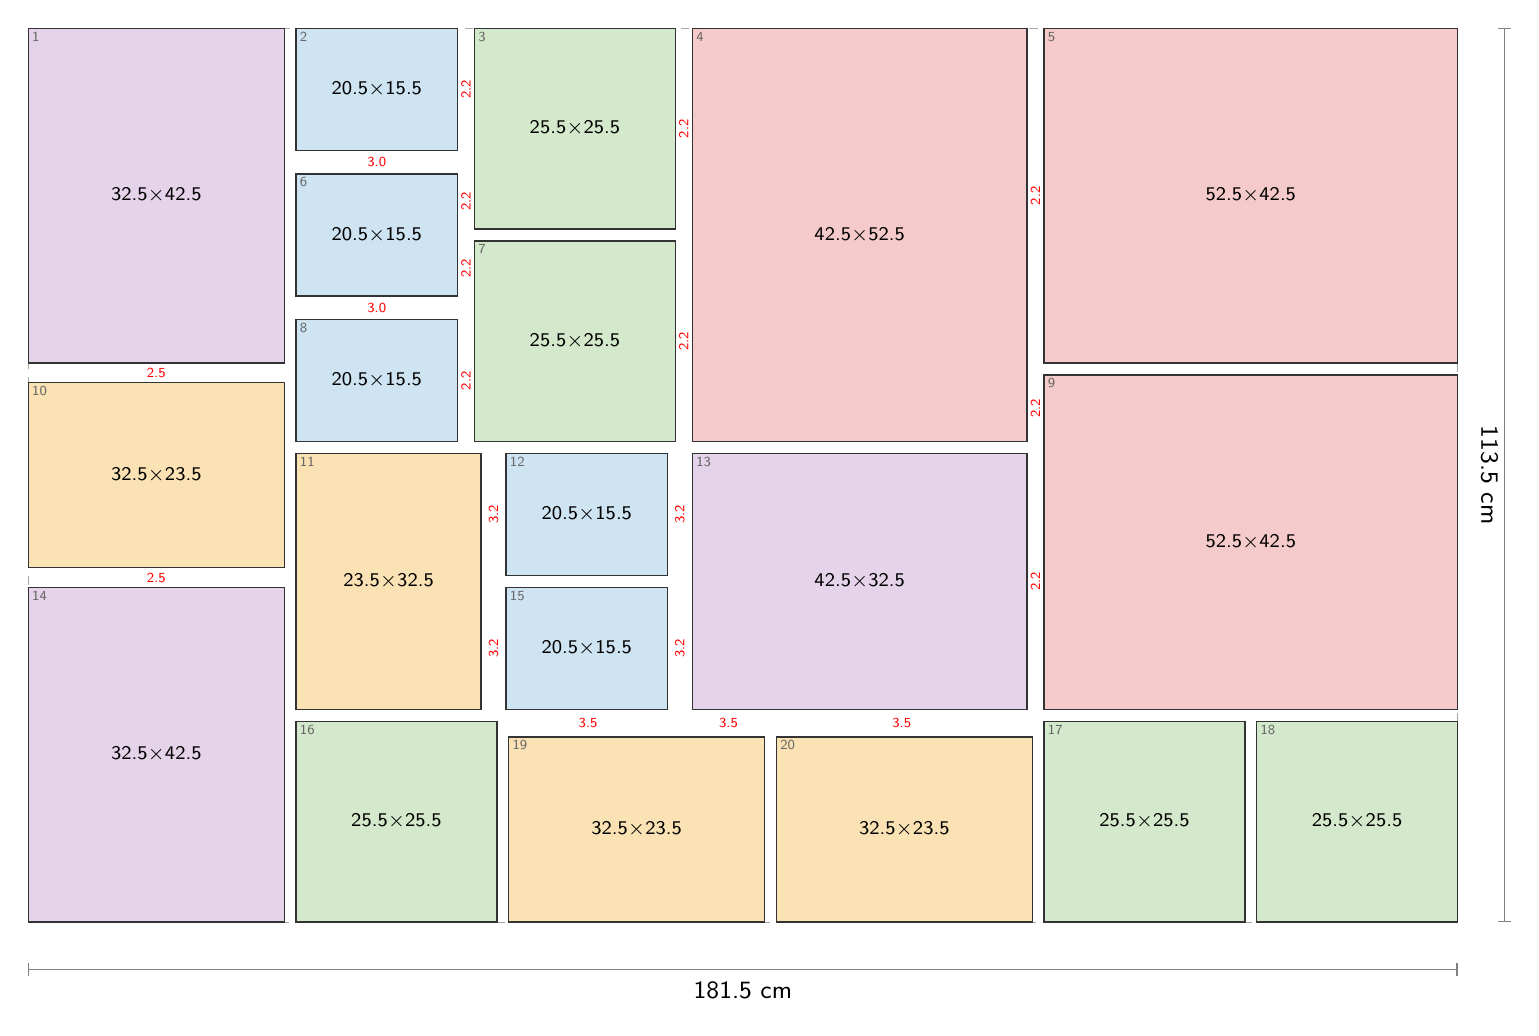
\begin{tikzpicture}[x=1mm, y=-1mm]
\draw[gray!70, dashed, line width=0.4pt] (0,0) rectangle (181.50,113.50);
\filldraw[fill=ft3, draw=black!80, line width=0.5pt] (0.00,0.00) rectangle (32.50,42.50);
\node[align=center, inner sep=0pt] at (16.25,21.25) {\scriptsize 32.5$\times$42.5};
\node[anchor=north west, inner sep=1.2pt, font=\tiny, text=black!60] at (0.00,0.00) {1};
\filldraw[fill=ft0, draw=black!80, line width=0.5pt] (34.00,0.00) rectangle (54.50,15.50);
\node[align=center, inner sep=0pt] at (44.25,7.75) {\scriptsize 20.5$\times$15.5};
\node[anchor=north west, inner sep=1.2pt, font=\tiny, text=black!60] at (34.00,0.00) {2};
\filldraw[fill=ft2, draw=black!80, line width=0.5pt] (56.67,0.00) rectangle (82.17,25.50);
\node[align=center, inner sep=0pt] at (69.42,12.75) {\scriptsize 25.5$\times$25.5};
\node[anchor=north west, inner sep=1.2pt, font=\tiny, text=black!60] at (56.67,0.00) {3};
\filldraw[fill=ft4, draw=black!80, line width=0.5pt] (84.33,0.00) rectangle (126.83,52.50);
\node[align=center, inner sep=0pt] at (105.58,26.25) {\scriptsize 42.5$\times$52.5};
\node[anchor=north west, inner sep=1.2pt, font=\tiny, text=black!60] at (84.33,0.00) {4};
\filldraw[fill=ft4, draw=black!80, line width=0.5pt] (129.00,0.00) rectangle (181.50,42.50);
\node[align=center, inner sep=0pt] at (155.25,21.25) {\scriptsize 52.5$\times$42.5};
\node[anchor=north west, inner sep=1.2pt, font=\tiny, text=black!60] at (129.00,0.00) {5};
\filldraw[fill=ft0, draw=black!80, line width=0.5pt] (34.00,18.50) rectangle (54.50,34.00);
\node[align=center, inner sep=0pt] at (44.25,26.25) {\scriptsize 20.5$\times$15.5};
\node[anchor=north west, inner sep=1.2pt, font=\tiny, text=black!60] at (34.00,18.50) {6};
\filldraw[fill=ft2, draw=black!80, line width=0.5pt] (56.67,27.00) rectangle (82.17,52.50);
\node[align=center, inner sep=0pt] at (69.42,39.75) {\scriptsize 25.5$\times$25.5};
\node[anchor=north west, inner sep=1.2pt, font=\tiny, text=black!60] at (56.67,27.00) {7};
\filldraw[fill=ft0, draw=black!80, line width=0.5pt] (34.00,37.00) rectangle (54.50,52.50);
\node[align=center, inner sep=0pt] at (44.25,44.75) {\scriptsize 20.5$\times$15.5};
\node[anchor=north west, inner sep=1.2pt, font=\tiny, text=black!60] at (34.00,37.00) {8};
\filldraw[fill=ft4, draw=black!80, line width=0.5pt] (129.00,44.00) rectangle (181.50,86.50);
\node[align=center, inner sep=0pt] at (155.25,65.25) {\scriptsize 52.5$\times$42.5};
\node[anchor=north west, inner sep=1.2pt, font=\tiny, text=black!60] at (129.00,44.00) {9};
\filldraw[fill=ft1, draw=black!80, line width=0.5pt] (0.00,45.00) rectangle (32.50,68.50);
\node[align=center, inner sep=0pt] at (16.25,56.75) {\scriptsize 32.5$\times$23.5};
\node[anchor=north west, inner sep=1.2pt, font=\tiny, text=black!60] at (0.00,45.00) {10};
\filldraw[fill=ft1, draw=black!80, line width=0.5pt] (34.00,54.00) rectangle (57.50,86.50);
\node[align=center, inner sep=0pt] at (45.75,70.25) {\scriptsize 23.5$\times$32.5};
\node[anchor=north west, inner sep=1.2pt, font=\tiny, text=black!60] at (34.00,54.00) {11};
\filldraw[fill=ft0, draw=black!80, line width=0.5pt] (60.67,54.00) rectangle (81.17,69.50);
\node[align=center, inner sep=0pt] at (70.92,61.75) {\scriptsize 20.5$\times$15.5};
\node[anchor=north west, inner sep=1.2pt, font=\tiny, text=black!60] at (60.67,54.00) {12};
\filldraw[fill=ft3, draw=black!80, line width=0.5pt] (84.33,54.00) rectangle (126.83,86.50);
\node[align=center, inner sep=0pt] at (105.58,70.25) {\scriptsize 42.5$\times$32.5};
\node[anchor=north west, inner sep=1.2pt, font=\tiny, text=black!60] at (84.33,54.00) {13};
\filldraw[fill=ft3, draw=black!80, line width=0.5pt] (0.00,71.00) rectangle (32.50,113.50);
\node[align=center, inner sep=0pt] at (16.25,92.25) {\scriptsize 32.5$\times$42.5};
\node[anchor=north west, inner sep=1.2pt, font=\tiny, text=black!60] at (0.00,71.00) {14};
\filldraw[fill=ft0, draw=black!80, line width=0.5pt] (60.67,71.00) rectangle (81.17,86.50);
\node[align=center, inner sep=0pt] at (70.92,78.75) {\scriptsize 20.5$\times$15.5};
\node[anchor=north west, inner sep=1.2pt, font=\tiny, text=black!60] at (60.67,71.00) {15};
\filldraw[fill=ft2, draw=black!80, line width=0.5pt] (34.00,88.00) rectangle (59.50,113.50);
\node[align=center, inner sep=0pt] at (46.75,100.75) {\scriptsize 25.5$\times$25.5};
\node[anchor=north west, inner sep=1.2pt, font=\tiny, text=black!60] at (34.00,88.00) {16};
\filldraw[fill=ft2, draw=black!80, line width=0.5pt] (129.00,88.00) rectangle (154.50,113.50);
\node[align=center, inner sep=0pt] at (141.75,100.75) {\scriptsize 25.5$\times$25.5};
\node[anchor=north west, inner sep=1.2pt, font=\tiny, text=black!60] at (129.00,88.00) {17};
\filldraw[fill=ft2, draw=black!80, line width=0.5pt] (156.00,88.00) rectangle (181.50,113.50);
\node[align=center, inner sep=0pt] at (168.75,100.75) {\scriptsize 25.5$\times$25.5};
\node[anchor=north west, inner sep=1.2pt, font=\tiny, text=black!60] at (156.00,88.00) {18};
\filldraw[fill=ft1, draw=black!80, line width=0.5pt] (61.00,90.00) rectangle (93.50,113.50);
\node[align=center, inner sep=0pt] at (77.25,101.75) {\scriptsize 32.5$\times$23.5};
\node[anchor=north west, inner sep=1.2pt, font=\tiny, text=black!60] at (61.00,90.00) {19};
\filldraw[fill=ft1, draw=black!80, line width=0.5pt] (95.00,90.00) rectangle (127.50,113.50);
\node[align=center, inner sep=0pt] at (111.25,101.75) {\scriptsize 32.5$\times$23.5};
\node[anchor=north west, inner sep=1.2pt, font=\tiny, text=black!60] at (95.00,90.00) {20};
\node[font=\tiny, text=red, fill=white, inner sep=0.3pt] at (16.25,43.75) {2.5};
\node[font=\tiny, text=red, fill=white, inner sep=0.3pt, rotate=90] at (55.58,7.75) {2.2};
\node[font=\tiny, text=red, fill=white, inner sep=0.3pt] at (44.25,17.00) {3.0};
\node[font=\tiny, text=red, fill=white, inner sep=0.3pt, rotate=90] at (83.25,12.75) {2.2};
\node[font=\tiny, text=red, fill=white, inner sep=0.3pt, rotate=90] at (127.92,21.25) {2.2};
\node[font=\tiny, text=red, fill=white, inner sep=0.3pt, rotate=90] at (127.92,48.25) {2.2};
\node[font=\tiny, text=red, fill=white, inner sep=0.3pt, rotate=90] at (55.58,22.00) {2.2};
\node[font=\tiny, text=red, fill=white, inner sep=0.3pt, rotate=90] at (55.58,30.50) {2.2};
\node[font=\tiny, text=red, fill=white, inner sep=0.3pt] at (44.25,35.50) {3.0};
\node[font=\tiny, text=red, fill=white, inner sep=0.3pt, rotate=90] at (83.25,39.75) {2.2};
\node[font=\tiny, text=red, fill=white, inner sep=0.3pt, rotate=90] at (55.58,44.75) {2.2};
\node[font=\tiny, text=red, fill=white, inner sep=0.3pt] at (16.25,69.75) {2.5};
\node[font=\tiny, text=red, fill=white, inner sep=0.3pt, rotate=90] at (59.08,61.75) {3.2};
\node[font=\tiny, text=red, fill=white, inner sep=0.3pt, rotate=90] at (59.08,78.75) {3.2};
\node[font=\tiny, text=red, fill=white, inner sep=0.3pt, rotate=90] at (82.75,61.75) {3.2};
\node[font=\tiny, text=red, fill=white, inner sep=0.3pt, rotate=90] at (127.92,70.25) {2.2};
\node[font=\tiny, text=red, fill=white, inner sep=0.3pt] at (88.92,88.25) {3.5};
\node[font=\tiny, text=red, fill=white, inner sep=0.3pt] at (110.92,88.25) {3.5};
\node[font=\tiny, text=red, fill=white, inner sep=0.3pt, rotate=90] at (82.75,78.75) {3.2};
\node[font=\tiny, text=red, fill=white, inner sep=0.3pt] at (71.08,88.25) {3.5};
\draw[Bar-Bar, gray] (0,119.50) -- (181.50,119.50) node[midway, below=1pt, font=\small, text=black] {181.5 cm};
\draw[Bar-Bar, gray] (187.50,0) -- (187.50,113.50) node[midway, right=1pt, font=\small, text=black, rotate=-90, anchor=north] {113.5 cm};
\end{tikzpicture}\\[4pt]
{\scriptsize Scale 1:10 (1 mm = 1 cm). Red numbers mark gaps that deviate from the nominal gap by more than 0.25 cm. Small grey numbers index the coordinate table.}
\end{minipage}\hfill
\begin{minipage}[t]{0.25\textwidth}\vspace{0pt}
\small
\begin{tabular}{@{}l l@{}}
\toprule
Outer size & 181.5 $\times$ 113.5 cm \\
Nominal gap & 1.5 cm \\
Actual gaps & 1.5 -- 3.5 cm \\
Max.\ deviation & 2.0 cm \\
Mean deviation & 0.59 cm \\
Border notches & none \\
Corners filled & 4 / 4 \\
Frames used & 20 of 28 \\
\bottomrule
\end{tabular}

\vspace{8pt}
\scriptsize
\begin{tabular}{@{}c l l r r@{}}
\toprule
 & outer w $\times$ h (cm) & & used & have \\
\midrule
\tikz[baseline=-0.6ex]\fill[ft0,draw=black!60] (0,0) rectangle (1.2ex,1.2ex); & 20.5$\times$15.5 & L & 5 & 9 \\
\tikz[baseline=-0.6ex]\fill[ft0,draw=black!60] (0,0) rectangle (1.2ex,1.2ex); & 15.5$\times$20.5 & P & 0 & 2 \\
\tikz[baseline=-0.6ex]\fill[ft3,draw=black!60] (0,0) rectangle (1.2ex,1.2ex); & 32.5$\times$42.5 & P & 2 & 2 \\
\tikz[baseline=-0.6ex]\fill[ft3,draw=black!60] (0,0) rectangle (1.2ex,1.2ex); & 42.5$\times$32.5 & L & 1 & 1 \\
\tikz[baseline=-0.6ex]\fill[ft1,draw=black!60] (0,0) rectangle (1.2ex,1.2ex); & 32.5$\times$23.5 & L & 3 & 5 \\
\tikz[baseline=-0.6ex]\fill[ft1,draw=black!60] (0,0) rectangle (1.2ex,1.2ex); & 23.5$\times$32.5 & P & 1 & 1 \\
\tikz[baseline=-0.6ex]\fill[ft2,draw=black!60] (0,0) rectangle (1.2ex,1.2ex); & 25.5$\times$25.5 &  & 5 & 5 \\
\tikz[baseline=-0.6ex]\fill[ft4,draw=black!60] (0,0) rectangle (1.2ex,1.2ex); & 42.5$\times$52.5 & P & 1 & 1 \\
\tikz[baseline=-0.6ex]\fill[ft4,draw=black!60] (0,0) rectangle (1.2ex,1.2ex); & 52.5$\times$42.5 & L & 2 & 2 \\
\bottomrule
\end{tabular}

\vspace{8pt}
{\bfseries Positions} (top-left corner, cm)\\[2pt]
\tiny
\begin{tabular}{@{}r l r r@{}}
\toprule
\# & frame w $\times$ h & x & y \\
\midrule
1 & 32.5 $\times$ 42.5 & 0.0 & 0.0 \\
2 & 20.5 $\times$ 15.5 & 34.0 & 0.0 \\
3 & 25.5 $\times$ 25.5 & 56.7 & 0.0 \\
4 & 42.5 $\times$ 52.5 & 84.3 & 0.0 \\
5 & 52.5 $\times$ 42.5 & 129.0 & 0.0 \\
6 & 20.5 $\times$ 15.5 & 34.0 & 18.5 \\
7 & 25.5 $\times$ 25.5 & 56.7 & 27.0 \\
8 & 20.5 $\times$ 15.5 & 34.0 & 37.0 \\
9 & 52.5 $\times$ 42.5 & 129.0 & 44.0 \\
10 & 32.5 $\times$ 23.5 & 0.0 & 45.0 \\
11 & 23.5 $\times$ 32.5 & 34.0 & 54.0 \\
12 & 20.5 $\times$ 15.5 & 60.7 & 54.0 \\
13 & 42.5 $\times$ 32.5 & 84.3 & 54.0 \\
14 & 32.5 $\times$ 42.5 & 0.0 & 71.0 \\
15 & 20.5 $\times$ 15.5 & 60.7 & 71.0 \\
16 & 25.5 $\times$ 25.5 & 34.0 & 88.0 \\
17 & 25.5 $\times$ 25.5 & 129.0 & 88.0 \\
18 & 25.5 $\times$ 25.5 & 156.0 & 88.0 \\
19 & 32.5 $\times$ 23.5 & 61.0 & 90.0 \\
20 & 32.5 $\times$ 23.5 & 95.0 & 90.0 \\
\bottomrule
\end{tabular}
\end{minipage}
\clearpage

\begin{minipage}[t]{0.74\textwidth}\vspace{0pt}
{\LARGE\bfseries Layout 8}\hspace{1.5em}{\large 181.5 $\times$ 113.5 cm \quad gap 1.5 cm \quad 20 frames}\\[8pt]
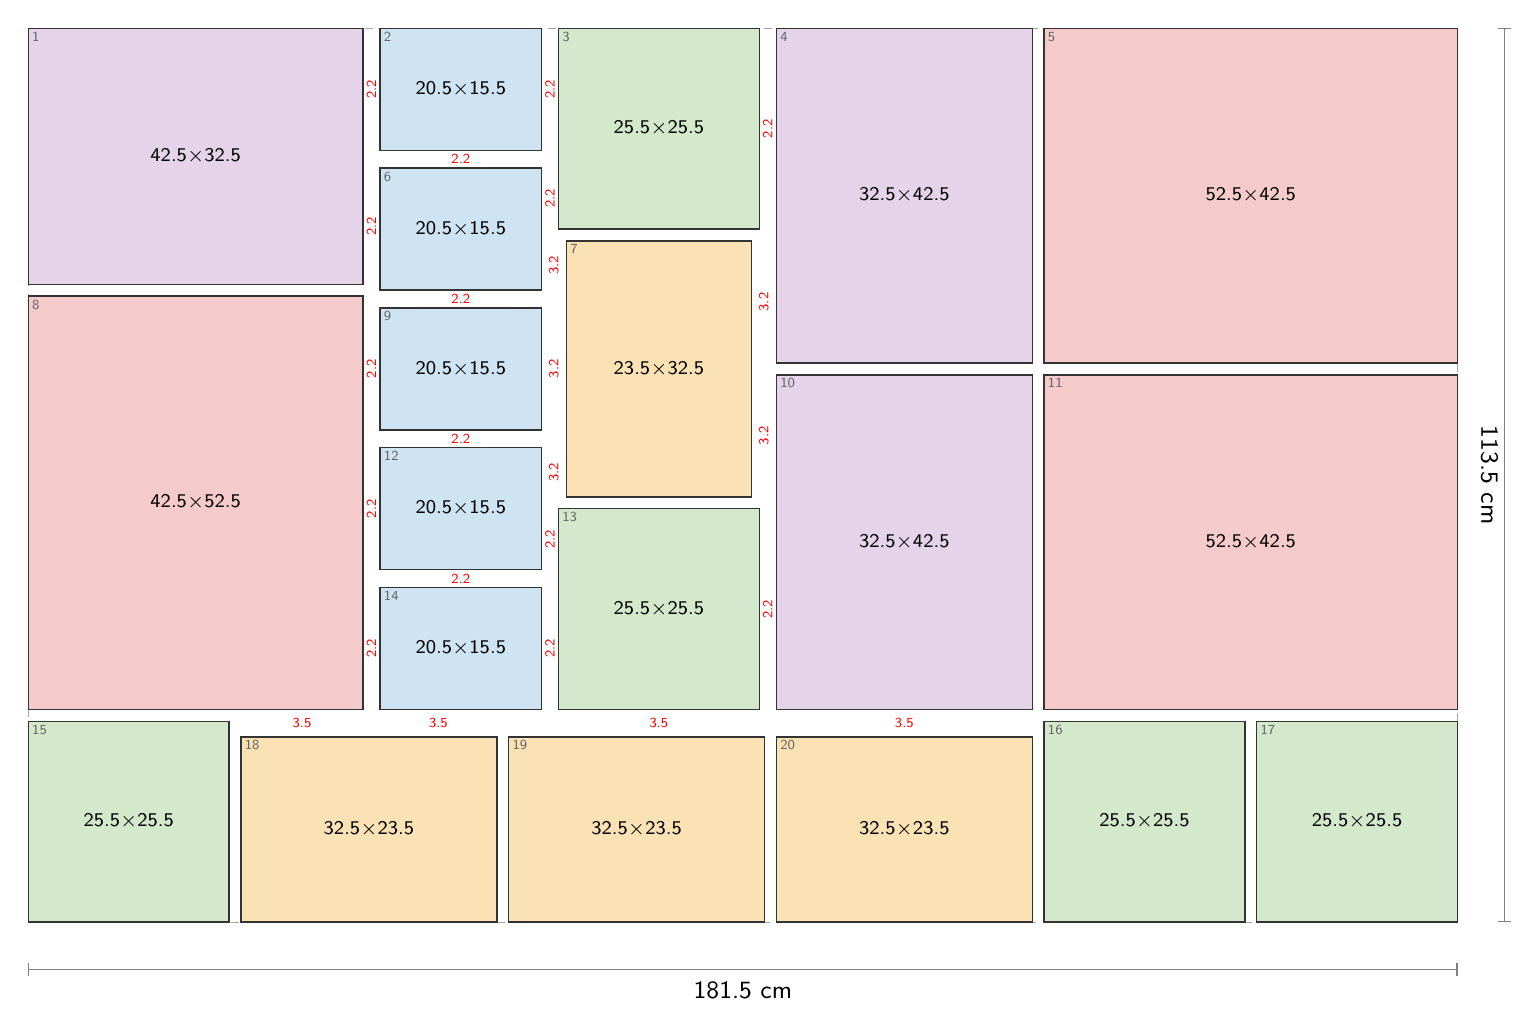
\begin{tikzpicture}[x=1mm, y=-1mm]
\draw[gray!70, dashed, line width=0.4pt] (0,0) rectangle (181.50,113.50);
\filldraw[fill=ft3, draw=black!80, line width=0.5pt] (0.00,0.00) rectangle (42.50,32.50);
\node[align=center, inner sep=0pt] at (21.25,16.25) {\scriptsize 42.5$\times$32.5};
\node[anchor=north west, inner sep=1.2pt, font=\tiny, text=black!60] at (0.00,0.00) {1};
\filldraw[fill=ft0, draw=black!80, line width=0.5pt] (44.67,0.00) rectangle (65.17,15.50);
\node[align=center, inner sep=0pt] at (54.92,7.75) {\scriptsize 20.5$\times$15.5};
\node[anchor=north west, inner sep=1.2pt, font=\tiny, text=black!60] at (44.67,0.00) {2};
\filldraw[fill=ft2, draw=black!80, line width=0.5pt] (67.33,0.00) rectangle (92.83,25.50);
\node[align=center, inner sep=0pt] at (80.08,12.75) {\scriptsize 25.5$\times$25.5};
\node[anchor=north west, inner sep=1.2pt, font=\tiny, text=black!60] at (67.33,0.00) {3};
\filldraw[fill=ft3, draw=black!80, line width=0.5pt] (95.00,0.00) rectangle (127.50,42.50);
\node[align=center, inner sep=0pt] at (111.25,21.25) {\scriptsize 32.5$\times$42.5};
\node[anchor=north west, inner sep=1.2pt, font=\tiny, text=black!60] at (95.00,0.00) {4};
\filldraw[fill=ft4, draw=black!80, line width=0.5pt] (129.00,0.00) rectangle (181.50,42.50);
\node[align=center, inner sep=0pt] at (155.25,21.25) {\scriptsize 52.5$\times$42.5};
\node[anchor=north west, inner sep=1.2pt, font=\tiny, text=black!60] at (129.00,0.00) {5};
\filldraw[fill=ft0, draw=black!80, line width=0.5pt] (44.67,17.75) rectangle (65.17,33.25);
\node[align=center, inner sep=0pt] at (54.92,25.50) {\scriptsize 20.5$\times$15.5};
\node[anchor=north west, inner sep=1.2pt, font=\tiny, text=black!60] at (44.67,17.75) {6};
\filldraw[fill=ft1, draw=black!80, line width=0.5pt] (68.33,27.00) rectangle (91.83,59.50);
\node[align=center, inner sep=0pt] at (80.08,43.25) {\scriptsize 23.5$\times$32.5};
\node[anchor=north west, inner sep=1.2pt, font=\tiny, text=black!60] at (68.33,27.00) {7};
\filldraw[fill=ft4, draw=black!80, line width=0.5pt] (0.00,34.00) rectangle (42.50,86.50);
\node[align=center, inner sep=0pt] at (21.25,60.25) {\scriptsize 42.5$\times$52.5};
\node[anchor=north west, inner sep=1.2pt, font=\tiny, text=black!60] at (0.00,34.00) {8};
\filldraw[fill=ft0, draw=black!80, line width=0.5pt] (44.67,35.50) rectangle (65.17,51.00);
\node[align=center, inner sep=0pt] at (54.92,43.25) {\scriptsize 20.5$\times$15.5};
\node[anchor=north west, inner sep=1.2pt, font=\tiny, text=black!60] at (44.67,35.50) {9};
\filldraw[fill=ft3, draw=black!80, line width=0.5pt] (95.00,44.00) rectangle (127.50,86.50);
\node[align=center, inner sep=0pt] at (111.25,65.25) {\scriptsize 32.5$\times$42.5};
\node[anchor=north west, inner sep=1.2pt, font=\tiny, text=black!60] at (95.00,44.00) {10};
\filldraw[fill=ft4, draw=black!80, line width=0.5pt] (129.00,44.00) rectangle (181.50,86.50);
\node[align=center, inner sep=0pt] at (155.25,65.25) {\scriptsize 52.5$\times$42.5};
\node[anchor=north west, inner sep=1.2pt, font=\tiny, text=black!60] at (129.00,44.00) {11};
\filldraw[fill=ft0, draw=black!80, line width=0.5pt] (44.67,53.25) rectangle (65.17,68.75);
\node[align=center, inner sep=0pt] at (54.92,61.00) {\scriptsize 20.5$\times$15.5};
\node[anchor=north west, inner sep=1.2pt, font=\tiny, text=black!60] at (44.67,53.25) {12};
\filldraw[fill=ft2, draw=black!80, line width=0.5pt] (67.33,61.00) rectangle (92.83,86.50);
\node[align=center, inner sep=0pt] at (80.08,73.75) {\scriptsize 25.5$\times$25.5};
\node[anchor=north west, inner sep=1.2pt, font=\tiny, text=black!60] at (67.33,61.00) {13};
\filldraw[fill=ft0, draw=black!80, line width=0.5pt] (44.67,71.00) rectangle (65.17,86.50);
\node[align=center, inner sep=0pt] at (54.92,78.75) {\scriptsize 20.5$\times$15.5};
\node[anchor=north west, inner sep=1.2pt, font=\tiny, text=black!60] at (44.67,71.00) {14};
\filldraw[fill=ft2, draw=black!80, line width=0.5pt] (0.00,88.00) rectangle (25.50,113.50);
\node[align=center, inner sep=0pt] at (12.75,100.75) {\scriptsize 25.5$\times$25.5};
\node[anchor=north west, inner sep=1.2pt, font=\tiny, text=black!60] at (0.00,88.00) {15};
\filldraw[fill=ft2, draw=black!80, line width=0.5pt] (129.00,88.00) rectangle (154.50,113.50);
\node[align=center, inner sep=0pt] at (141.75,100.75) {\scriptsize 25.5$\times$25.5};
\node[anchor=north west, inner sep=1.2pt, font=\tiny, text=black!60] at (129.00,88.00) {16};
\filldraw[fill=ft2, draw=black!80, line width=0.5pt] (156.00,88.00) rectangle (181.50,113.50);
\node[align=center, inner sep=0pt] at (168.75,100.75) {\scriptsize 25.5$\times$25.5};
\node[anchor=north west, inner sep=1.2pt, font=\tiny, text=black!60] at (156.00,88.00) {17};
\filldraw[fill=ft1, draw=black!80, line width=0.5pt] (27.00,90.00) rectangle (59.50,113.50);
\node[align=center, inner sep=0pt] at (43.25,101.75) {\scriptsize 32.5$\times$23.5};
\node[anchor=north west, inner sep=1.2pt, font=\tiny, text=black!60] at (27.00,90.00) {18};
\filldraw[fill=ft1, draw=black!80, line width=0.5pt] (61.00,90.00) rectangle (93.50,113.50);
\node[align=center, inner sep=0pt] at (77.25,101.75) {\scriptsize 32.5$\times$23.5};
\node[anchor=north west, inner sep=1.2pt, font=\tiny, text=black!60] at (61.00,90.00) {19};
\filldraw[fill=ft1, draw=black!80, line width=0.5pt] (95.00,90.00) rectangle (127.50,113.50);
\node[align=center, inner sep=0pt] at (111.25,101.75) {\scriptsize 32.5$\times$23.5};
\node[anchor=north west, inner sep=1.2pt, font=\tiny, text=black!60] at (95.00,90.00) {20};
\node[font=\tiny, text=red, fill=white, inner sep=0.3pt, rotate=90] at (43.58,7.75) {2.2};
\node[font=\tiny, text=red, fill=white, inner sep=0.3pt, rotate=90] at (43.58,25.12) {2.2};
\node[font=\tiny, text=red, fill=white, inner sep=0.3pt, rotate=90] at (66.25,7.75) {2.2};
\node[font=\tiny, text=red, fill=white, inner sep=0.3pt] at (54.92,16.62) {2.2};
\node[font=\tiny, text=red, fill=white, inner sep=0.3pt, rotate=90] at (93.92,12.75) {2.2};
\node[font=\tiny, text=red, fill=white, inner sep=0.3pt, rotate=90] at (66.25,21.62) {2.2};
\node[font=\tiny, text=red, fill=white, inner sep=0.3pt, rotate=90] at (66.75,30.12) {3.2};
\node[font=\tiny, text=red, fill=white, inner sep=0.3pt] at (54.92,34.38) {2.2};
\node[font=\tiny, text=red, fill=white, inner sep=0.3pt, rotate=90] at (93.42,34.75) {3.2};
\node[font=\tiny, text=red, fill=white, inner sep=0.3pt, rotate=90] at (93.42,51.75) {3.2};
\node[font=\tiny, text=red, fill=white, inner sep=0.3pt, rotate=90] at (43.58,43.25) {2.2};
\node[font=\tiny, text=red, fill=white, inner sep=0.3pt, rotate=90] at (43.58,61.00) {2.2};
\node[font=\tiny, text=red, fill=white, inner sep=0.3pt, rotate=90] at (43.58,78.75) {2.2};
\node[font=\tiny, text=red, fill=white, inner sep=0.3pt] at (34.75,88.25) {3.5};
\node[font=\tiny, text=red, fill=white, inner sep=0.3pt, rotate=90] at (66.75,43.25) {3.2};
\node[font=\tiny, text=red, fill=white, inner sep=0.3pt] at (54.92,52.12) {2.2};
\node[font=\tiny, text=red, fill=white, inner sep=0.3pt] at (111.25,88.25) {3.5};
\node[font=\tiny, text=red, fill=white, inner sep=0.3pt, rotate=90] at (66.75,56.38) {3.2};
\node[font=\tiny, text=red, fill=white, inner sep=0.3pt, rotate=90] at (66.25,64.88) {2.2};
\node[font=\tiny, text=red, fill=white, inner sep=0.3pt] at (54.92,69.88) {2.2};
\node[font=\tiny, text=red, fill=white, inner sep=0.3pt, rotate=90] at (93.92,73.75) {2.2};
\node[font=\tiny, text=red, fill=white, inner sep=0.3pt] at (80.08,88.25) {3.5};
\node[font=\tiny, text=red, fill=white, inner sep=0.3pt, rotate=90] at (66.25,78.75) {2.2};
\node[font=\tiny, text=red, fill=white, inner sep=0.3pt] at (52.08,88.25) {3.5};
\draw[Bar-Bar, gray] (0,119.50) -- (181.50,119.50) node[midway, below=1pt, font=\small, text=black] {181.5 cm};
\draw[Bar-Bar, gray] (187.50,0) -- (187.50,113.50) node[midway, right=1pt, font=\small, text=black, rotate=-90, anchor=north] {113.5 cm};
\end{tikzpicture}\\[4pt]
{\scriptsize Scale 1:10 (1 mm = 1 cm). Red numbers mark gaps that deviate from the nominal gap by more than 0.25 cm. Small grey numbers index the coordinate table.}
\end{minipage}\hfill
\begin{minipage}[t]{0.25\textwidth}\vspace{0pt}
\small
\begin{tabular}{@{}l l@{}}
\toprule
Outer size & 181.5 $\times$ 113.5 cm \\
Nominal gap & 1.5 cm \\
Actual gaps & 1.5 -- 3.5 cm \\
Max.\ deviation & 2.0 cm \\
Mean deviation & 0.68 cm \\
Border notches & none \\
Corners filled & 4 / 4 \\
Frames used & 20 of 28 \\
\bottomrule
\end{tabular}

\vspace{8pt}
\scriptsize
\begin{tabular}{@{}c l l r r@{}}
\toprule
 & outer w $\times$ h (cm) & & used & have \\
\midrule
\tikz[baseline=-0.6ex]\fill[ft0,draw=black!60] (0,0) rectangle (1.2ex,1.2ex); & 20.5$\times$15.5 & L & 5 & 9 \\
\tikz[baseline=-0.6ex]\fill[ft0,draw=black!60] (0,0) rectangle (1.2ex,1.2ex); & 15.5$\times$20.5 & P & 0 & 2 \\
\tikz[baseline=-0.6ex]\fill[ft3,draw=black!60] (0,0) rectangle (1.2ex,1.2ex); & 32.5$\times$42.5 & P & 2 & 2 \\
\tikz[baseline=-0.6ex]\fill[ft3,draw=black!60] (0,0) rectangle (1.2ex,1.2ex); & 42.5$\times$32.5 & L & 1 & 1 \\
\tikz[baseline=-0.6ex]\fill[ft1,draw=black!60] (0,0) rectangle (1.2ex,1.2ex); & 32.5$\times$23.5 & L & 3 & 5 \\
\tikz[baseline=-0.6ex]\fill[ft1,draw=black!60] (0,0) rectangle (1.2ex,1.2ex); & 23.5$\times$32.5 & P & 1 & 1 \\
\tikz[baseline=-0.6ex]\fill[ft2,draw=black!60] (0,0) rectangle (1.2ex,1.2ex); & 25.5$\times$25.5 &  & 5 & 5 \\
\tikz[baseline=-0.6ex]\fill[ft4,draw=black!60] (0,0) rectangle (1.2ex,1.2ex); & 42.5$\times$52.5 & P & 1 & 1 \\
\tikz[baseline=-0.6ex]\fill[ft4,draw=black!60] (0,0) rectangle (1.2ex,1.2ex); & 52.5$\times$42.5 & L & 2 & 2 \\
\bottomrule
\end{tabular}

\vspace{8pt}
{\bfseries Positions} (top-left corner, cm)\\[2pt]
\tiny
\begin{tabular}{@{}r l r r@{}}
\toprule
\# & frame w $\times$ h & x & y \\
\midrule
1 & 42.5 $\times$ 32.5 & 0.0 & 0.0 \\
2 & 20.5 $\times$ 15.5 & 44.7 & 0.0 \\
3 & 25.5 $\times$ 25.5 & 67.3 & 0.0 \\
4 & 32.5 $\times$ 42.5 & 95.0 & 0.0 \\
5 & 52.5 $\times$ 42.5 & 129.0 & 0.0 \\
6 & 20.5 $\times$ 15.5 & 44.7 & 17.8 \\
7 & 23.5 $\times$ 32.5 & 68.3 & 27.0 \\
8 & 42.5 $\times$ 52.5 & 0.0 & 34.0 \\
9 & 20.5 $\times$ 15.5 & 44.7 & 35.5 \\
10 & 32.5 $\times$ 42.5 & 95.0 & 44.0 \\
11 & 52.5 $\times$ 42.5 & 129.0 & 44.0 \\
12 & 20.5 $\times$ 15.5 & 44.7 & 53.2 \\
13 & 25.5 $\times$ 25.5 & 67.3 & 61.0 \\
14 & 20.5 $\times$ 15.5 & 44.7 & 71.0 \\
15 & 25.5 $\times$ 25.5 & 0.0 & 88.0 \\
16 & 25.5 $\times$ 25.5 & 129.0 & 88.0 \\
17 & 25.5 $\times$ 25.5 & 156.0 & 88.0 \\
18 & 32.5 $\times$ 23.5 & 27.0 & 90.0 \\
19 & 32.5 $\times$ 23.5 & 61.0 & 90.0 \\
20 & 32.5 $\times$ 23.5 & 95.0 & 90.0 \\
\bottomrule
\end{tabular}
\end{minipage}
\clearpage

\begin{minipage}[t]{0.74\textwidth}\vspace{0pt}
{\LARGE\bfseries Layout 9}\hspace{1.5em}{\large 179.5 $\times$ 120.5 cm \quad gap 1.5 cm \quad 26 frames}\\[8pt]
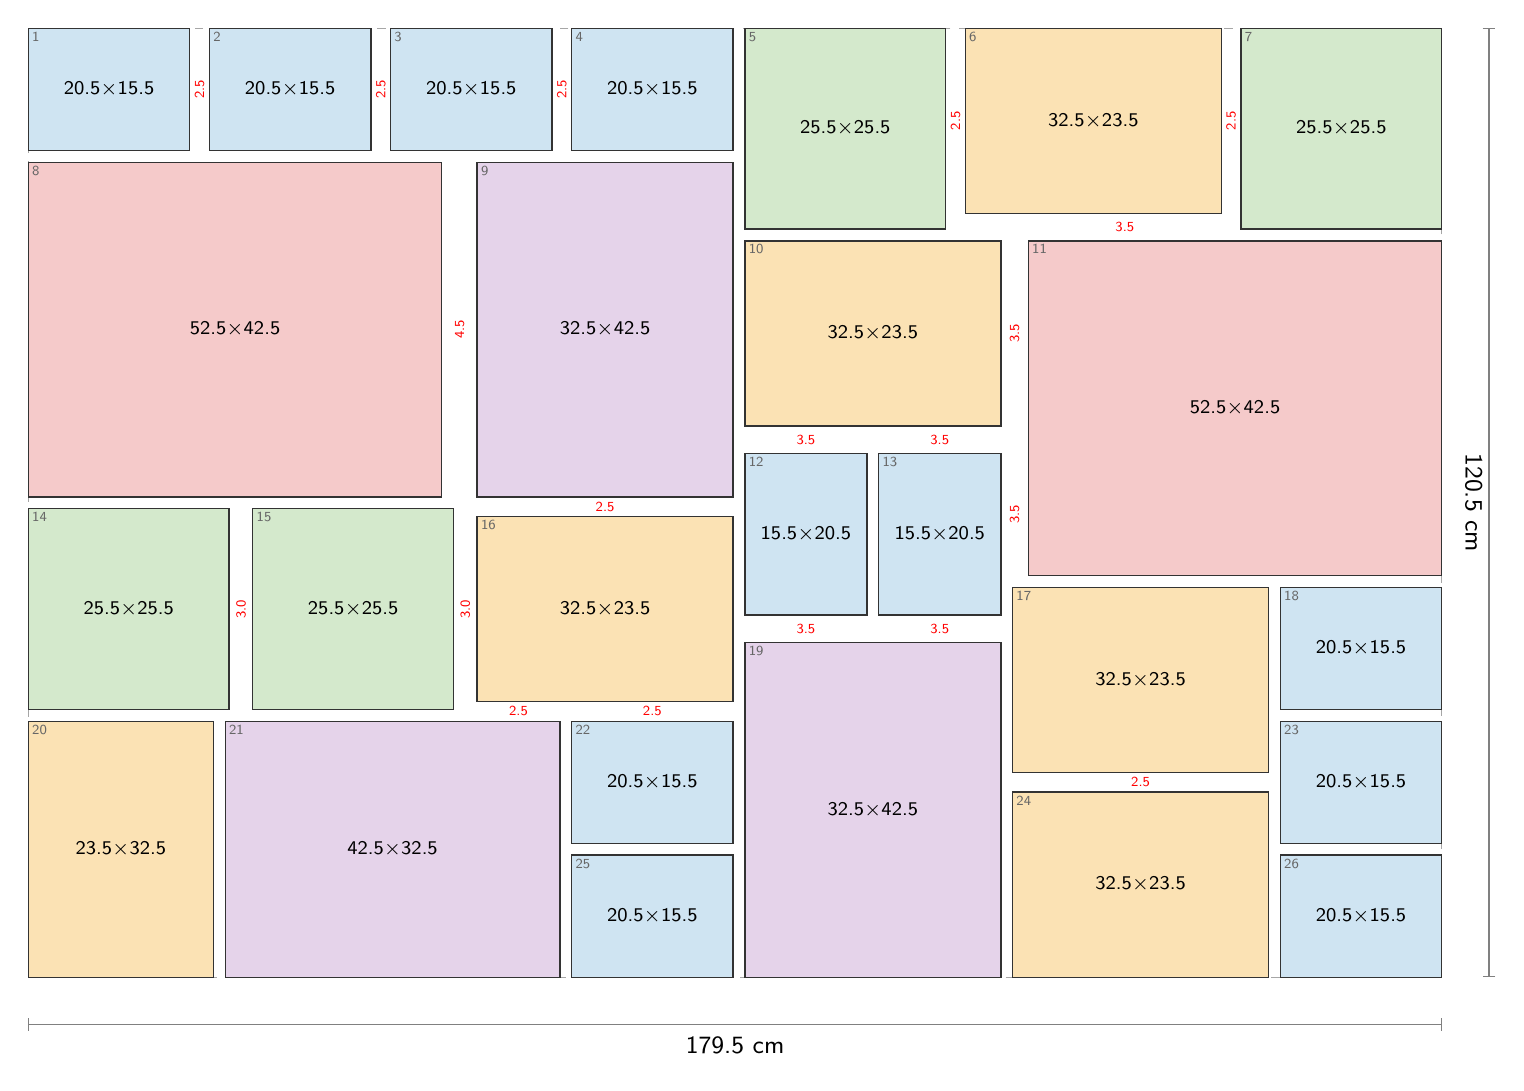
\begin{tikzpicture}[x=1mm, y=-1mm]
\draw[gray!70, dashed, line width=0.4pt] (0,0) rectangle (179.50,120.50);
\filldraw[fill=ft0, draw=black!80, line width=0.5pt] (0.00,0.00) rectangle (20.50,15.50);
\node[align=center, inner sep=0pt] at (10.25,7.75) {\scriptsize 20.5$\times$15.5};
\node[anchor=north west, inner sep=1.2pt, font=\tiny, text=black!60] at (0.00,0.00) {1};
\filldraw[fill=ft0, draw=black!80, line width=0.5pt] (23.00,0.00) rectangle (43.50,15.50);
\node[align=center, inner sep=0pt] at (33.25,7.75) {\scriptsize 20.5$\times$15.5};
\node[anchor=north west, inner sep=1.2pt, font=\tiny, text=black!60] at (23.00,0.00) {2};
\filldraw[fill=ft0, draw=black!80, line width=0.5pt] (46.00,0.00) rectangle (66.50,15.50);
\node[align=center, inner sep=0pt] at (56.25,7.75) {\scriptsize 20.5$\times$15.5};
\node[anchor=north west, inner sep=1.2pt, font=\tiny, text=black!60] at (46.00,0.00) {3};
\filldraw[fill=ft0, draw=black!80, line width=0.5pt] (69.00,0.00) rectangle (89.50,15.50);
\node[align=center, inner sep=0pt] at (79.25,7.75) {\scriptsize 20.5$\times$15.5};
\node[anchor=north west, inner sep=1.2pt, font=\tiny, text=black!60] at (69.00,0.00) {4};
\filldraw[fill=ft2, draw=black!80, line width=0.5pt] (91.00,0.00) rectangle (116.50,25.50);
\node[align=center, inner sep=0pt] at (103.75,12.75) {\scriptsize 25.5$\times$25.5};
\node[anchor=north west, inner sep=1.2pt, font=\tiny, text=black!60] at (91.00,0.00) {5};
\filldraw[fill=ft1, draw=black!80, line width=0.5pt] (119.00,0.00) rectangle (151.50,23.50);
\node[align=center, inner sep=0pt] at (135.25,11.75) {\scriptsize 32.5$\times$23.5};
\node[anchor=north west, inner sep=1.2pt, font=\tiny, text=black!60] at (119.00,0.00) {6};
\filldraw[fill=ft2, draw=black!80, line width=0.5pt] (154.00,0.00) rectangle (179.50,25.50);
\node[align=center, inner sep=0pt] at (166.75,12.75) {\scriptsize 25.5$\times$25.5};
\node[anchor=north west, inner sep=1.2pt, font=\tiny, text=black!60] at (154.00,0.00) {7};
\filldraw[fill=ft4, draw=black!80, line width=0.5pt] (0.00,17.00) rectangle (52.50,59.50);
\node[align=center, inner sep=0pt] at (26.25,38.25) {\scriptsize 52.5$\times$42.5};
\node[anchor=north west, inner sep=1.2pt, font=\tiny, text=black!60] at (0.00,17.00) {8};
\filldraw[fill=ft3, draw=black!80, line width=0.5pt] (57.00,17.00) rectangle (89.50,59.50);
\node[align=center, inner sep=0pt] at (73.25,38.25) {\scriptsize 32.5$\times$42.5};
\node[anchor=north west, inner sep=1.2pt, font=\tiny, text=black!60] at (57.00,17.00) {9};
\filldraw[fill=ft1, draw=black!80, line width=0.5pt] (91.00,27.00) rectangle (123.50,50.50);
\node[align=center, inner sep=0pt] at (107.25,38.75) {\scriptsize 32.5$\times$23.5};
\node[anchor=north west, inner sep=1.2pt, font=\tiny, text=black!60] at (91.00,27.00) {10};
\filldraw[fill=ft4, draw=black!80, line width=0.5pt] (127.00,27.00) rectangle (179.50,69.50);
\node[align=center, inner sep=0pt] at (153.25,48.25) {\scriptsize 52.5$\times$42.5};
\node[anchor=north west, inner sep=1.2pt, font=\tiny, text=black!60] at (127.00,27.00) {11};
\filldraw[fill=ft0, draw=black!80, line width=0.5pt] (91.00,54.00) rectangle (106.50,74.50);
\node[align=center, inner sep=0pt] at (98.75,64.25) {\scriptsize 15.5$\times$20.5};
\node[anchor=north west, inner sep=1.2pt, font=\tiny, text=black!60] at (91.00,54.00) {12};
\filldraw[fill=ft0, draw=black!80, line width=0.5pt] (108.00,54.00) rectangle (123.50,74.50);
\node[align=center, inner sep=0pt] at (115.75,64.25) {\scriptsize 15.5$\times$20.5};
\node[anchor=north west, inner sep=1.2pt, font=\tiny, text=black!60] at (108.00,54.00) {13};
\filldraw[fill=ft2, draw=black!80, line width=0.5pt] (0.00,61.00) rectangle (25.50,86.50);
\node[align=center, inner sep=0pt] at (12.75,73.75) {\scriptsize 25.5$\times$25.5};
\node[anchor=north west, inner sep=1.2pt, font=\tiny, text=black!60] at (0.00,61.00) {14};
\filldraw[fill=ft2, draw=black!80, line width=0.5pt] (28.50,61.00) rectangle (54.00,86.50);
\node[align=center, inner sep=0pt] at (41.25,73.75) {\scriptsize 25.5$\times$25.5};
\node[anchor=north west, inner sep=1.2pt, font=\tiny, text=black!60] at (28.50,61.00) {15};
\filldraw[fill=ft1, draw=black!80, line width=0.5pt] (57.00,62.00) rectangle (89.50,85.50);
\node[align=center, inner sep=0pt] at (73.25,73.75) {\scriptsize 32.5$\times$23.5};
\node[anchor=north west, inner sep=1.2pt, font=\tiny, text=black!60] at (57.00,62.00) {16};
\filldraw[fill=ft1, draw=black!80, line width=0.5pt] (125.00,71.00) rectangle (157.50,94.50);
\node[align=center, inner sep=0pt] at (141.25,82.75) {\scriptsize 32.5$\times$23.5};
\node[anchor=north west, inner sep=1.2pt, font=\tiny, text=black!60] at (125.00,71.00) {17};
\filldraw[fill=ft0, draw=black!80, line width=0.5pt] (159.00,71.00) rectangle (179.50,86.50);
\node[align=center, inner sep=0pt] at (169.25,78.75) {\scriptsize 20.5$\times$15.5};
\node[anchor=north west, inner sep=1.2pt, font=\tiny, text=black!60] at (159.00,71.00) {18};
\filldraw[fill=ft3, draw=black!80, line width=0.5pt] (91.00,78.00) rectangle (123.50,120.50);
\node[align=center, inner sep=0pt] at (107.25,99.25) {\scriptsize 32.5$\times$42.5};
\node[anchor=north west, inner sep=1.2pt, font=\tiny, text=black!60] at (91.00,78.00) {19};
\filldraw[fill=ft1, draw=black!80, line width=0.5pt] (0.00,88.00) rectangle (23.50,120.50);
\node[align=center, inner sep=0pt] at (11.75,104.25) {\scriptsize 23.5$\times$32.5};
\node[anchor=north west, inner sep=1.2pt, font=\tiny, text=black!60] at (0.00,88.00) {20};
\filldraw[fill=ft3, draw=black!80, line width=0.5pt] (25.00,88.00) rectangle (67.50,120.50);
\node[align=center, inner sep=0pt] at (46.25,104.25) {\scriptsize 42.5$\times$32.5};
\node[anchor=north west, inner sep=1.2pt, font=\tiny, text=black!60] at (25.00,88.00) {21};
\filldraw[fill=ft0, draw=black!80, line width=0.5pt] (69.00,88.00) rectangle (89.50,103.50);
\node[align=center, inner sep=0pt] at (79.25,95.75) {\scriptsize 20.5$\times$15.5};
\node[anchor=north west, inner sep=1.2pt, font=\tiny, text=black!60] at (69.00,88.00) {22};
\filldraw[fill=ft0, draw=black!80, line width=0.5pt] (159.00,88.00) rectangle (179.50,103.50);
\node[align=center, inner sep=0pt] at (169.25,95.75) {\scriptsize 20.5$\times$15.5};
\node[anchor=north west, inner sep=1.2pt, font=\tiny, text=black!60] at (159.00,88.00) {23};
\filldraw[fill=ft1, draw=black!80, line width=0.5pt] (125.00,97.00) rectangle (157.50,120.50);
\node[align=center, inner sep=0pt] at (141.25,108.75) {\scriptsize 32.5$\times$23.5};
\node[anchor=north west, inner sep=1.2pt, font=\tiny, text=black!60] at (125.00,97.00) {24};
\filldraw[fill=ft0, draw=black!80, line width=0.5pt] (69.00,105.00) rectangle (89.50,120.50);
\node[align=center, inner sep=0pt] at (79.25,112.75) {\scriptsize 20.5$\times$15.5};
\node[anchor=north west, inner sep=1.2pt, font=\tiny, text=black!60] at (69.00,105.00) {25};
\filldraw[fill=ft0, draw=black!80, line width=0.5pt] (159.00,105.00) rectangle (179.50,120.50);
\node[align=center, inner sep=0pt] at (169.25,112.75) {\scriptsize 20.5$\times$15.5};
\node[anchor=north west, inner sep=1.2pt, font=\tiny, text=black!60] at (159.00,105.00) {26};
\node[font=\tiny, text=red, fill=white, inner sep=0.3pt, rotate=90] at (21.75,7.75) {2.5};
\node[font=\tiny, text=red, fill=white, inner sep=0.3pt, rotate=90] at (44.75,7.75) {2.5};
\node[font=\tiny, text=red, fill=white, inner sep=0.3pt, rotate=90] at (67.75,7.75) {2.5};
\node[font=\tiny, text=red, fill=white, inner sep=0.3pt, rotate=90] at (117.75,11.75) {2.5};
\node[font=\tiny, text=red, fill=white, inner sep=0.3pt, rotate=90] at (152.75,11.75) {2.5};
\node[font=\tiny, text=red, fill=white, inner sep=0.3pt] at (139.25,25.25) {3.5};
\node[font=\tiny, text=red, fill=white, inner sep=0.3pt, rotate=90] at (54.75,38.25) {4.5};
\node[font=\tiny, text=red, fill=white, inner sep=0.3pt] at (73.25,60.75) {2.5};
\node[font=\tiny, text=red, fill=white, inner sep=0.3pt, rotate=90] at (125.25,38.75) {3.5};
\node[font=\tiny, text=red, fill=white, inner sep=0.3pt] at (98.75,52.25) {3.5};
\node[font=\tiny, text=red, fill=white, inner sep=0.3pt] at (115.75,52.25) {3.5};
\node[font=\tiny, text=red, fill=white, inner sep=0.3pt] at (98.75,76.25) {3.5};
\node[font=\tiny, text=red, fill=white, inner sep=0.3pt, rotate=90] at (125.25,61.75) {3.5};
\node[font=\tiny, text=red, fill=white, inner sep=0.3pt] at (115.75,76.25) {3.5};
\node[font=\tiny, text=red, fill=white, inner sep=0.3pt, rotate=90] at (27.00,73.75) {3.0};
\node[font=\tiny, text=red, fill=white, inner sep=0.3pt, rotate=90] at (55.50,73.75) {3.0};
\node[font=\tiny, text=red, fill=white, inner sep=0.3pt] at (62.25,86.75) {2.5};
\node[font=\tiny, text=red, fill=white, inner sep=0.3pt] at (79.25,86.75) {2.5};
\node[font=\tiny, text=red, fill=white, inner sep=0.3pt] at (141.25,95.75) {2.5};
\draw[Bar-Bar, gray] (0,126.50) -- (179.50,126.50) node[midway, below=1pt, font=\small, text=black] {179.5 cm};
\draw[Bar-Bar, gray] (185.50,0) -- (185.50,120.50) node[midway, right=1pt, font=\small, text=black, rotate=-90, anchor=north] {120.5 cm};
\end{tikzpicture}\\[4pt]
{\scriptsize Scale 1:10 (1 mm = 1 cm). Red numbers mark gaps that deviate from the nominal gap by more than 0.25 cm. Small grey numbers index the coordinate table.}
\end{minipage}\hfill
\begin{minipage}[t]{0.25\textwidth}\vspace{0pt}
\small
\begin{tabular}{@{}l l@{}}
\toprule
Outer size & 179.5 $\times$ 120.5 cm \\
Nominal gap & 1.5 cm \\
Actual gaps & 1.5 -- 4.5 cm \\
Max.\ deviation & 3.0 cm \\
Mean deviation & 0.55 cm \\
Border notches & none \\
Corners filled & 4 / 4 \\
Frames used & 26 of 28 \\
\bottomrule
\end{tabular}

\vspace{8pt}
\scriptsize
\begin{tabular}{@{}c l l r r@{}}
\toprule
 & outer w $\times$ h (cm) & & used & have \\
\midrule
\tikz[baseline=-0.6ex]\fill[ft0,draw=black!60] (0,0) rectangle (1.2ex,1.2ex); & 20.5$\times$15.5 & L & 9 & 9 \\
\tikz[baseline=-0.6ex]\fill[ft0,draw=black!60] (0,0) rectangle (1.2ex,1.2ex); & 15.5$\times$20.5 & P & 2 & 2 \\
\tikz[baseline=-0.6ex]\fill[ft3,draw=black!60] (0,0) rectangle (1.2ex,1.2ex); & 32.5$\times$42.5 & P & 2 & 2 \\
\tikz[baseline=-0.6ex]\fill[ft3,draw=black!60] (0,0) rectangle (1.2ex,1.2ex); & 42.5$\times$32.5 & L & 1 & 1 \\
\tikz[baseline=-0.6ex]\fill[ft1,draw=black!60] (0,0) rectangle (1.2ex,1.2ex); & 32.5$\times$23.5 & L & 5 & 5 \\
\tikz[baseline=-0.6ex]\fill[ft1,draw=black!60] (0,0) rectangle (1.2ex,1.2ex); & 23.5$\times$32.5 & P & 1 & 1 \\
\tikz[baseline=-0.6ex]\fill[ft2,draw=black!60] (0,0) rectangle (1.2ex,1.2ex); & 25.5$\times$25.5 &  & 4 & 5 \\
\tikz[baseline=-0.6ex]\fill[ft4,draw=black!60] (0,0) rectangle (1.2ex,1.2ex); & 42.5$\times$52.5 & P & 0 & 1 \\
\tikz[baseline=-0.6ex]\fill[ft4,draw=black!60] (0,0) rectangle (1.2ex,1.2ex); & 52.5$\times$42.5 & L & 2 & 2 \\
\bottomrule
\end{tabular}

\vspace{8pt}
{\bfseries Positions} (top-left corner, cm)\\[2pt]
\tiny
\begin{tabular}{@{}r l r r@{}}
\toprule
\# & frame w $\times$ h & x & y \\
\midrule
1 & 20.5 $\times$ 15.5 & 0.0 & 0.0 \\
2 & 20.5 $\times$ 15.5 & 23.0 & 0.0 \\
3 & 20.5 $\times$ 15.5 & 46.0 & 0.0 \\
4 & 20.5 $\times$ 15.5 & 69.0 & 0.0 \\
5 & 25.5 $\times$ 25.5 & 91.0 & 0.0 \\
6 & 32.5 $\times$ 23.5 & 119.0 & 0.0 \\
7 & 25.5 $\times$ 25.5 & 154.0 & 0.0 \\
8 & 52.5 $\times$ 42.5 & 0.0 & 17.0 \\
9 & 32.5 $\times$ 42.5 & 57.0 & 17.0 \\
10 & 32.5 $\times$ 23.5 & 91.0 & 27.0 \\
11 & 52.5 $\times$ 42.5 & 127.0 & 27.0 \\
12 & 15.5 $\times$ 20.5 & 91.0 & 54.0 \\
13 & 15.5 $\times$ 20.5 & 108.0 & 54.0 \\
14 & 25.5 $\times$ 25.5 & 0.0 & 61.0 \\
15 & 25.5 $\times$ 25.5 & 28.5 & 61.0 \\
16 & 32.5 $\times$ 23.5 & 57.0 & 62.0 \\
17 & 32.5 $\times$ 23.5 & 125.0 & 71.0 \\
18 & 20.5 $\times$ 15.5 & 159.0 & 71.0 \\
19 & 32.5 $\times$ 42.5 & 91.0 & 78.0 \\
20 & 23.5 $\times$ 32.5 & 0.0 & 88.0 \\
21 & 42.5 $\times$ 32.5 & 25.0 & 88.0 \\
22 & 20.5 $\times$ 15.5 & 69.0 & 88.0 \\
23 & 20.5 $\times$ 15.5 & 159.0 & 88.0 \\
24 & 32.5 $\times$ 23.5 & 125.0 & 97.0 \\
25 & 20.5 $\times$ 15.5 & 69.0 & 105.0 \\
26 & 20.5 $\times$ 15.5 & 159.0 & 105.0 \\
\bottomrule
\end{tabular}
\end{minipage}
\clearpage

\begin{minipage}[t]{0.74\textwidth}\vspace{0pt}
{\LARGE\bfseries Layout 10}\hspace{1.5em}{\large 181.5 $\times$ 114.5 cm \quad gap 1.5 cm \quad 25 frames}\\[8pt]
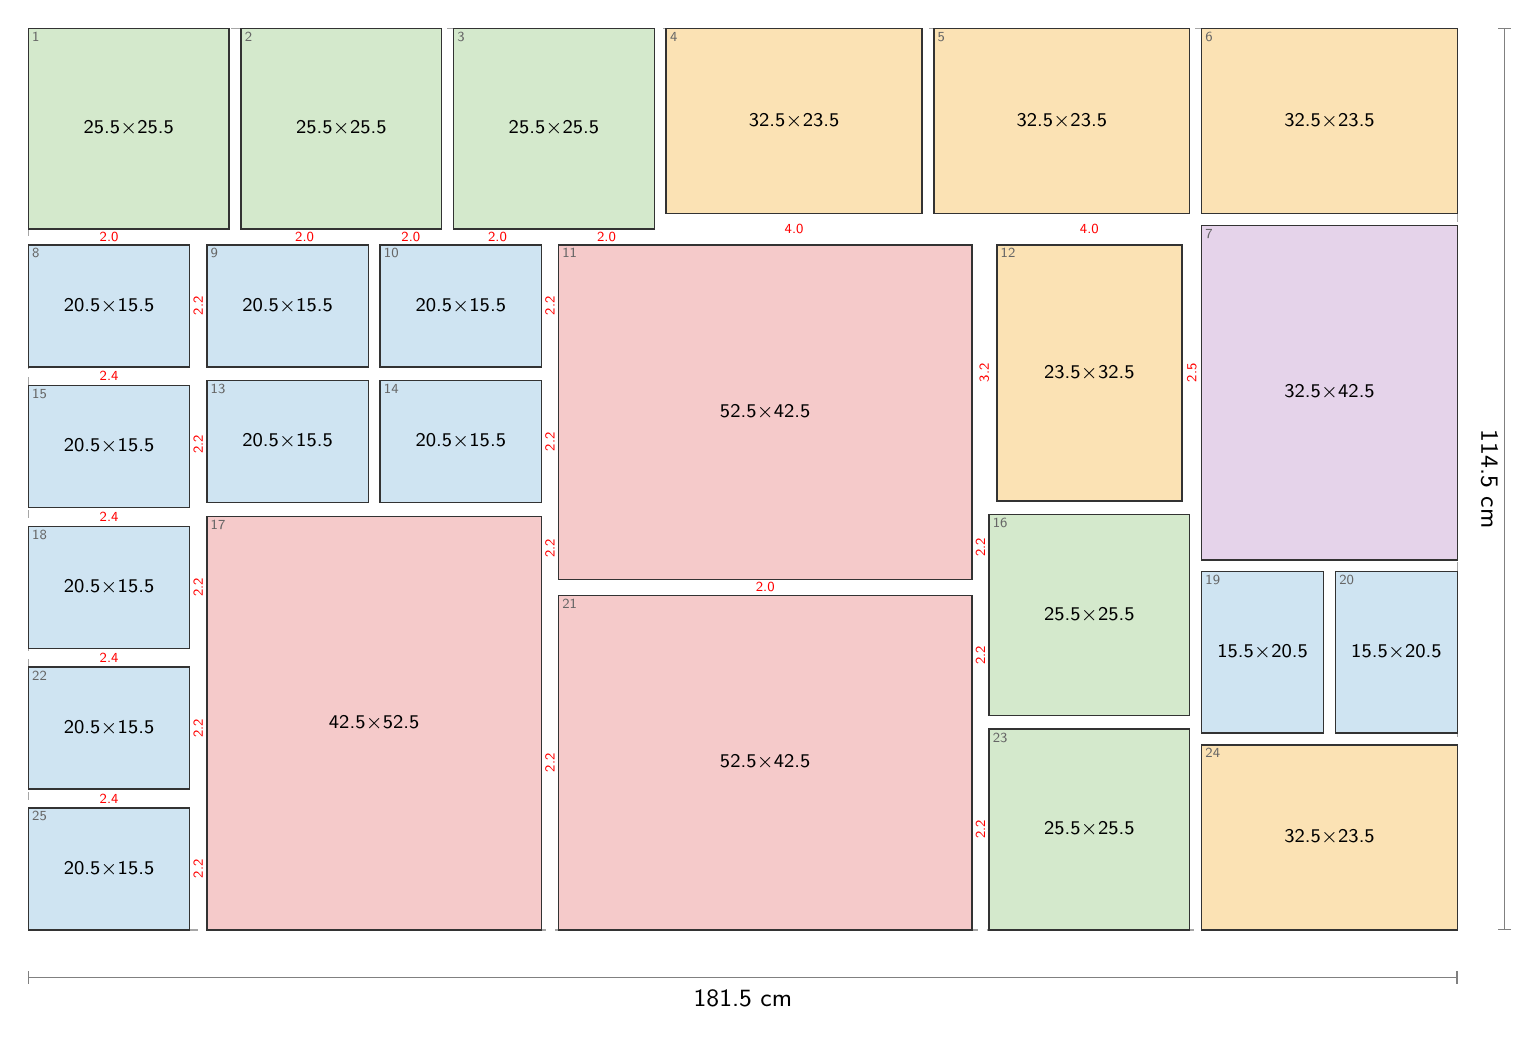
\begin{tikzpicture}[x=1mm, y=-1mm]
\draw[gray!70, dashed, line width=0.4pt] (0,0) rectangle (181.50,114.50);
\filldraw[fill=ft2, draw=black!80, line width=0.5pt] (0.00,0.00) rectangle (25.50,25.50);
\node[align=center, inner sep=0pt] at (12.75,12.75) {\scriptsize 25.5$\times$25.5};
\node[anchor=north west, inner sep=1.2pt, font=\tiny, text=black!60] at (0.00,0.00) {1};
\filldraw[fill=ft2, draw=black!80, line width=0.5pt] (27.00,0.00) rectangle (52.50,25.50);
\node[align=center, inner sep=0pt] at (39.75,12.75) {\scriptsize 25.5$\times$25.5};
\node[anchor=north west, inner sep=1.2pt, font=\tiny, text=black!60] at (27.00,0.00) {2};
\filldraw[fill=ft2, draw=black!80, line width=0.5pt] (54.00,0.00) rectangle (79.50,25.50);
\node[align=center, inner sep=0pt] at (66.75,12.75) {\scriptsize 25.5$\times$25.5};
\node[anchor=north west, inner sep=1.2pt, font=\tiny, text=black!60] at (54.00,0.00) {3};
\filldraw[fill=ft1, draw=black!80, line width=0.5pt] (81.00,0.00) rectangle (113.50,23.50);
\node[align=center, inner sep=0pt] at (97.25,11.75) {\scriptsize 32.5$\times$23.5};
\node[anchor=north west, inner sep=1.2pt, font=\tiny, text=black!60] at (81.00,0.00) {4};
\filldraw[fill=ft1, draw=black!80, line width=0.5pt] (115.00,0.00) rectangle (147.50,23.50);
\node[align=center, inner sep=0pt] at (131.25,11.75) {\scriptsize 32.5$\times$23.5};
\node[anchor=north west, inner sep=1.2pt, font=\tiny, text=black!60] at (115.00,0.00) {5};
\filldraw[fill=ft1, draw=black!80, line width=0.5pt] (149.00,0.00) rectangle (181.50,23.50);
\node[align=center, inner sep=0pt] at (165.25,11.75) {\scriptsize 32.5$\times$23.5};
\node[anchor=north west, inner sep=1.2pt, font=\tiny, text=black!60] at (149.00,0.00) {6};
\filldraw[fill=ft3, draw=black!80, line width=0.5pt] (149.00,25.00) rectangle (181.50,67.50);
\node[align=center, inner sep=0pt] at (165.25,46.25) {\scriptsize 32.5$\times$42.5};
\node[anchor=north west, inner sep=1.2pt, font=\tiny, text=black!60] at (149.00,25.00) {7};
\filldraw[fill=ft0, draw=black!80, line width=0.5pt] (0.00,27.50) rectangle (20.50,43.00);
\node[align=center, inner sep=0pt] at (10.25,35.25) {\scriptsize 20.5$\times$15.5};
\node[anchor=north west, inner sep=1.2pt, font=\tiny, text=black!60] at (0.00,27.50) {8};
\filldraw[fill=ft0, draw=black!80, line width=0.5pt] (22.67,27.50) rectangle (43.17,43.00);
\node[align=center, inner sep=0pt] at (32.92,35.25) {\scriptsize 20.5$\times$15.5};
\node[anchor=north west, inner sep=1.2pt, font=\tiny, text=black!60] at (22.67,27.50) {9};
\filldraw[fill=ft0, draw=black!80, line width=0.5pt] (44.67,27.50) rectangle (65.17,43.00);
\node[align=center, inner sep=0pt] at (54.92,35.25) {\scriptsize 20.5$\times$15.5};
\node[anchor=north west, inner sep=1.2pt, font=\tiny, text=black!60] at (44.67,27.50) {10};
\filldraw[fill=ft4, draw=black!80, line width=0.5pt] (67.33,27.50) rectangle (119.83,70.00);
\node[align=center, inner sep=0pt] at (93.58,48.75) {\scriptsize 52.5$\times$42.5};
\node[anchor=north west, inner sep=1.2pt, font=\tiny, text=black!60] at (67.33,27.50) {11};
\filldraw[fill=ft1, draw=black!80, line width=0.5pt] (123.00,27.50) rectangle (146.50,60.00);
\node[align=center, inner sep=0pt] at (134.75,43.75) {\scriptsize 23.5$\times$32.5};
\node[anchor=north west, inner sep=1.2pt, font=\tiny, text=black!60] at (123.00,27.50) {12};
\filldraw[fill=ft0, draw=black!80, line width=0.5pt] (22.67,44.75) rectangle (43.17,60.25);
\node[align=center, inner sep=0pt] at (32.92,52.50) {\scriptsize 20.5$\times$15.5};
\node[anchor=north west, inner sep=1.2pt, font=\tiny, text=black!60] at (22.67,44.75) {13};
\filldraw[fill=ft0, draw=black!80, line width=0.5pt] (44.67,44.75) rectangle (65.17,60.25);
\node[align=center, inner sep=0pt] at (54.92,52.50) {\scriptsize 20.5$\times$15.5};
\node[anchor=north west, inner sep=1.2pt, font=\tiny, text=black!60] at (44.67,44.75) {14};
\filldraw[fill=ft0, draw=black!80, line width=0.5pt] (0.00,45.38) rectangle (20.50,60.88);
\node[align=center, inner sep=0pt] at (10.25,53.12) {\scriptsize 20.5$\times$15.5};
\node[anchor=north west, inner sep=1.2pt, font=\tiny, text=black!60] at (0.00,45.38) {15};
\filldraw[fill=ft2, draw=black!80, line width=0.5pt] (122.00,61.75) rectangle (147.50,87.25);
\node[align=center, inner sep=0pt] at (134.75,74.50) {\scriptsize 25.5$\times$25.5};
\node[anchor=north west, inner sep=1.2pt, font=\tiny, text=black!60] at (122.00,61.75) {16};
\filldraw[fill=ft4, draw=black!80, line width=0.5pt] (22.67,62.00) rectangle (65.17,114.50);
\node[align=center, inner sep=0pt] at (43.92,88.25) {\scriptsize 42.5$\times$52.5};
\node[anchor=north west, inner sep=1.2pt, font=\tiny, text=black!60] at (22.67,62.00) {17};
\filldraw[fill=ft0, draw=black!80, line width=0.5pt] (0.00,63.25) rectangle (20.50,78.75);
\node[align=center, inner sep=0pt] at (10.25,71.00) {\scriptsize 20.5$\times$15.5};
\node[anchor=north west, inner sep=1.2pt, font=\tiny, text=black!60] at (0.00,63.25) {18};
\filldraw[fill=ft0, draw=black!80, line width=0.5pt] (149.00,69.00) rectangle (164.50,89.50);
\node[align=center, inner sep=0pt] at (156.75,79.25) {\scriptsize 15.5$\times$20.5};
\node[anchor=north west, inner sep=1.2pt, font=\tiny, text=black!60] at (149.00,69.00) {19};
\filldraw[fill=ft0, draw=black!80, line width=0.5pt] (166.00,69.00) rectangle (181.50,89.50);
\node[align=center, inner sep=0pt] at (173.75,79.25) {\scriptsize 15.5$\times$20.5};
\node[anchor=north west, inner sep=1.2pt, font=\tiny, text=black!60] at (166.00,69.00) {20};
\filldraw[fill=ft4, draw=black!80, line width=0.5pt] (67.33,72.00) rectangle (119.83,114.50);
\node[align=center, inner sep=0pt] at (93.58,93.25) {\scriptsize 52.5$\times$42.5};
\node[anchor=north west, inner sep=1.2pt, font=\tiny, text=black!60] at (67.33,72.00) {21};
\filldraw[fill=ft0, draw=black!80, line width=0.5pt] (0.00,81.12) rectangle (20.50,96.62);
\node[align=center, inner sep=0pt] at (10.25,88.88) {\scriptsize 20.5$\times$15.5};
\node[anchor=north west, inner sep=1.2pt, font=\tiny, text=black!60] at (0.00,81.12) {22};
\filldraw[fill=ft2, draw=black!80, line width=0.5pt] (122.00,89.00) rectangle (147.50,114.50);
\node[align=center, inner sep=0pt] at (134.75,101.75) {\scriptsize 25.5$\times$25.5};
\node[anchor=north west, inner sep=1.2pt, font=\tiny, text=black!60] at (122.00,89.00) {23};
\filldraw[fill=ft1, draw=black!80, line width=0.5pt] (149.00,91.00) rectangle (181.50,114.50);
\node[align=center, inner sep=0pt] at (165.25,102.75) {\scriptsize 32.5$\times$23.5};
\node[anchor=north west, inner sep=1.2pt, font=\tiny, text=black!60] at (149.00,91.00) {24};
\filldraw[fill=ft0, draw=black!80, line width=0.5pt] (0.00,99.00) rectangle (20.50,114.50);
\node[align=center, inner sep=0pt] at (10.25,106.75) {\scriptsize 20.5$\times$15.5};
\node[anchor=north west, inner sep=1.2pt, font=\tiny, text=black!60] at (0.00,99.00) {25};
\node[font=\tiny, text=red, fill=white, inner sep=0.3pt] at (10.25,26.50) {2.0};
\node[font=\tiny, text=red, fill=white, inner sep=0.3pt] at (35.08,26.50) {2.0};
\node[font=\tiny, text=red, fill=white, inner sep=0.3pt] at (48.58,26.50) {2.0};
\node[font=\tiny, text=red, fill=white, inner sep=0.3pt] at (59.58,26.50) {2.0};
\node[font=\tiny, text=red, fill=white, inner sep=0.3pt] at (73.42,26.50) {2.0};
\node[font=\tiny, text=red, fill=white, inner sep=0.3pt] at (97.25,25.50) {4.0};
\node[font=\tiny, text=red, fill=white, inner sep=0.3pt] at (134.75,25.50) {4.0};
\node[font=\tiny, text=red, fill=white, inner sep=0.3pt, rotate=90] at (21.58,35.25) {2.2};
\node[font=\tiny, text=red, fill=white, inner sep=0.3pt] at (10.25,44.19) {2.4};
\node[font=\tiny, text=red, fill=white, inner sep=0.3pt, rotate=90] at (66.25,35.25) {2.2};
\node[font=\tiny, text=red, fill=white, inner sep=0.3pt, rotate=90] at (121.42,43.75) {3.2};
\node[font=\tiny, text=red, fill=white, inner sep=0.3pt, rotate=90] at (120.92,65.88) {2.2};
\node[font=\tiny, text=red, fill=white, inner sep=0.3pt] at (93.58,71.00) {2.0};
\node[font=\tiny, text=red, fill=white, inner sep=0.3pt, rotate=90] at (147.75,43.75) {2.5};
\node[font=\tiny, text=red, fill=white, inner sep=0.3pt, rotate=90] at (66.25,52.50) {2.2};
\node[font=\tiny, text=red, fill=white, inner sep=0.3pt, rotate=90] at (21.58,52.81) {2.2};
\node[font=\tiny, text=red, fill=white, inner sep=0.3pt] at (10.25,62.06) {2.4};
\node[font=\tiny, text=red, fill=white, inner sep=0.3pt, rotate=90] at (66.25,66.00) {2.2};
\node[font=\tiny, text=red, fill=white, inner sep=0.3pt, rotate=90] at (66.25,93.25) {2.2};
\node[font=\tiny, text=red, fill=white, inner sep=0.3pt, rotate=90] at (21.58,71.00) {2.2};
\node[font=\tiny, text=red, fill=white, inner sep=0.3pt] at (10.25,79.94) {2.4};
\node[font=\tiny, text=red, fill=white, inner sep=0.3pt, rotate=90] at (120.92,79.62) {2.2};
\node[font=\tiny, text=red, fill=white, inner sep=0.3pt, rotate=90] at (120.92,101.75) {2.2};
\node[font=\tiny, text=red, fill=white, inner sep=0.3pt, rotate=90] at (21.58,88.88) {2.2};
\node[font=\tiny, text=red, fill=white, inner sep=0.3pt] at (10.25,97.81) {2.4};
\node[font=\tiny, text=red, fill=white, inner sep=0.3pt, rotate=90] at (21.58,106.75) {2.2};
\draw[Bar-Bar, gray] (0,120.50) -- (181.50,120.50) node[midway, below=1pt, font=\small, text=black] {181.5 cm};
\draw[Bar-Bar, gray] (187.50,0) -- (187.50,114.50) node[midway, right=1pt, font=\small, text=black, rotate=-90, anchor=north] {114.5 cm};
\end{tikzpicture}\\[4pt]
{\scriptsize Scale 1:10 (1 mm = 1 cm). Red numbers mark gaps that deviate from the nominal gap by more than 0.25 cm. Small grey numbers index the coordinate table.}
\end{minipage}\hfill
\begin{minipage}[t]{0.25\textwidth}\vspace{0pt}
\small
\begin{tabular}{@{}l l@{}}
\toprule
Outer size & 181.5 $\times$ 114.5 cm \\
Nominal gap & 1.5 cm \\
Actual gaps & 1.5 -- 4.0 cm \\
Max.\ deviation & 2.5 cm \\
Mean deviation & 0.49 cm \\
Border notches & none \\
Corners filled & 4 / 4 \\
Frames used & 25 of 28 \\
\bottomrule
\end{tabular}

\vspace{8pt}
\scriptsize
\begin{tabular}{@{}c l l r r@{}}
\toprule
 & outer w $\times$ h (cm) & & used & have \\
\midrule
\tikz[baseline=-0.6ex]\fill[ft0,draw=black!60] (0,0) rectangle (1.2ex,1.2ex); & 20.5$\times$15.5 & L & 9 & 9 \\
\tikz[baseline=-0.6ex]\fill[ft0,draw=black!60] (0,0) rectangle (1.2ex,1.2ex); & 15.5$\times$20.5 & P & 2 & 2 \\
\tikz[baseline=-0.6ex]\fill[ft3,draw=black!60] (0,0) rectangle (1.2ex,1.2ex); & 32.5$\times$42.5 & P & 1 & 2 \\
\tikz[baseline=-0.6ex]\fill[ft3,draw=black!60] (0,0) rectangle (1.2ex,1.2ex); & 42.5$\times$32.5 & L & 0 & 1 \\
\tikz[baseline=-0.6ex]\fill[ft1,draw=black!60] (0,0) rectangle (1.2ex,1.2ex); & 32.5$\times$23.5 & L & 4 & 5 \\
\tikz[baseline=-0.6ex]\fill[ft1,draw=black!60] (0,0) rectangle (1.2ex,1.2ex); & 23.5$\times$32.5 & P & 1 & 1 \\
\tikz[baseline=-0.6ex]\fill[ft2,draw=black!60] (0,0) rectangle (1.2ex,1.2ex); & 25.5$\times$25.5 &  & 5 & 5 \\
\tikz[baseline=-0.6ex]\fill[ft4,draw=black!60] (0,0) rectangle (1.2ex,1.2ex); & 42.5$\times$52.5 & P & 1 & 1 \\
\tikz[baseline=-0.6ex]\fill[ft4,draw=black!60] (0,0) rectangle (1.2ex,1.2ex); & 52.5$\times$42.5 & L & 2 & 2 \\
\bottomrule
\end{tabular}

\vspace{8pt}
{\bfseries Positions} (top-left corner, cm)\\[2pt]
\tiny
\begin{tabular}{@{}r l r r@{}}
\toprule
\# & frame w $\times$ h & x & y \\
\midrule
1 & 25.5 $\times$ 25.5 & 0.0 & 0.0 \\
2 & 25.5 $\times$ 25.5 & 27.0 & 0.0 \\
3 & 25.5 $\times$ 25.5 & 54.0 & 0.0 \\
4 & 32.5 $\times$ 23.5 & 81.0 & 0.0 \\
5 & 32.5 $\times$ 23.5 & 115.0 & 0.0 \\
6 & 32.5 $\times$ 23.5 & 149.0 & 0.0 \\
7 & 32.5 $\times$ 42.5 & 149.0 & 25.0 \\
8 & 20.5 $\times$ 15.5 & 0.0 & 27.5 \\
9 & 20.5 $\times$ 15.5 & 22.7 & 27.5 \\
10 & 20.5 $\times$ 15.5 & 44.7 & 27.5 \\
11 & 52.5 $\times$ 42.5 & 67.3 & 27.5 \\
12 & 23.5 $\times$ 32.5 & 123.0 & 27.5 \\
13 & 20.5 $\times$ 15.5 & 22.7 & 44.8 \\
14 & 20.5 $\times$ 15.5 & 44.7 & 44.8 \\
15 & 20.5 $\times$ 15.5 & 0.0 & 45.4 \\
16 & 25.5 $\times$ 25.5 & 122.0 & 61.8 \\
17 & 42.5 $\times$ 52.5 & 22.7 & 62.0 \\
18 & 20.5 $\times$ 15.5 & 0.0 & 63.2 \\
19 & 15.5 $\times$ 20.5 & 149.0 & 69.0 \\
20 & 15.5 $\times$ 20.5 & 166.0 & 69.0 \\
21 & 52.5 $\times$ 42.5 & 67.3 & 72.0 \\
22 & 20.5 $\times$ 15.5 & 0.0 & 81.1 \\
23 & 25.5 $\times$ 25.5 & 122.0 & 89.0 \\
24 & 32.5 $\times$ 23.5 & 149.0 & 91.0 \\
25 & 20.5 $\times$ 15.5 & 0.0 & 99.0 \\
\bottomrule
\end{tabular}
\end{minipage}
\clearpage

\begin{minipage}[t]{0.74\textwidth}\vspace{0pt}
{\LARGE\bfseries Layout 11}\hspace{1.5em}{\large 181.5 $\times$ 114.5 cm \quad gap 1.5 cm \quad 25 frames}\\[8pt]
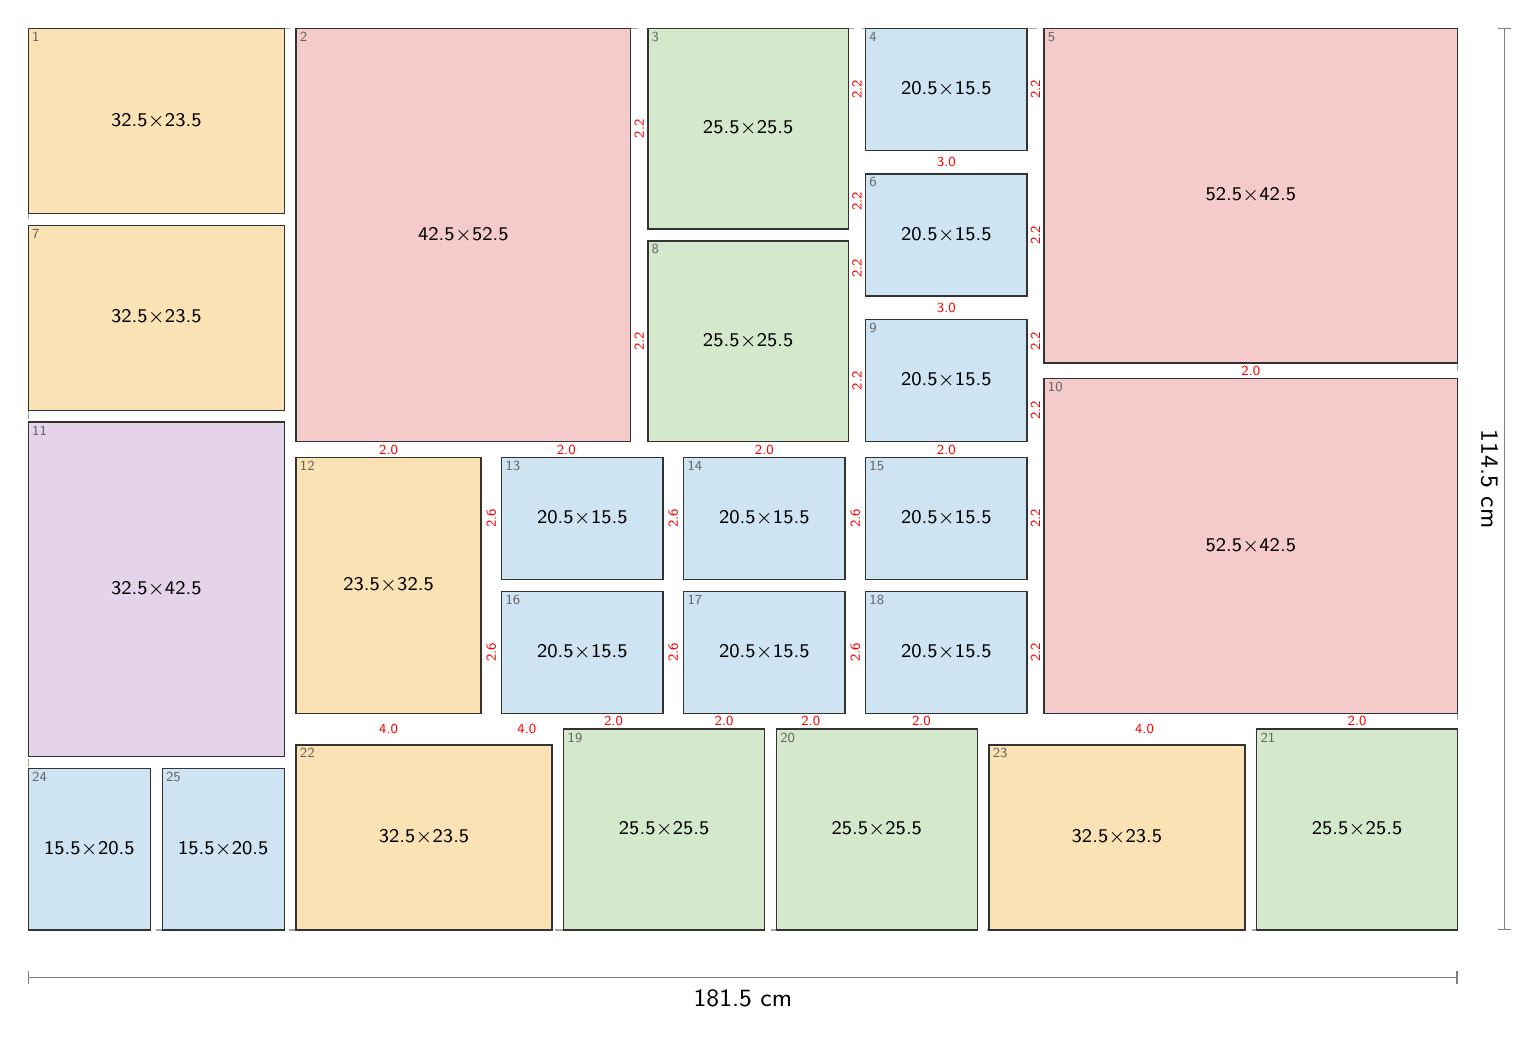
\begin{tikzpicture}[x=1mm, y=-1mm]
\draw[gray!70, dashed, line width=0.4pt] (0,0) rectangle (181.50,114.50);
\filldraw[fill=ft1, draw=black!80, line width=0.5pt] (0.00,0.00) rectangle (32.50,23.50);
\node[align=center, inner sep=0pt] at (16.25,11.75) {\scriptsize 32.5$\times$23.5};
\node[anchor=north west, inner sep=1.2pt, font=\tiny, text=black!60] at (0.00,0.00) {1};
\filldraw[fill=ft4, draw=black!80, line width=0.5pt] (34.00,0.00) rectangle (76.50,52.50);
\node[align=center, inner sep=0pt] at (55.25,26.25) {\scriptsize 42.5$\times$52.5};
\node[anchor=north west, inner sep=1.2pt, font=\tiny, text=black!60] at (34.00,0.00) {2};
\filldraw[fill=ft2, draw=black!80, line width=0.5pt] (78.67,0.00) rectangle (104.17,25.50);
\node[align=center, inner sep=0pt] at (91.42,12.75) {\scriptsize 25.5$\times$25.5};
\node[anchor=north west, inner sep=1.2pt, font=\tiny, text=black!60] at (78.67,0.00) {3};
\filldraw[fill=ft0, draw=black!80, line width=0.5pt] (106.33,0.00) rectangle (126.83,15.50);
\node[align=center, inner sep=0pt] at (116.58,7.75) {\scriptsize 20.5$\times$15.5};
\node[anchor=north west, inner sep=1.2pt, font=\tiny, text=black!60] at (106.33,0.00) {4};
\filldraw[fill=ft4, draw=black!80, line width=0.5pt] (129.00,0.00) rectangle (181.50,42.50);
\node[align=center, inner sep=0pt] at (155.25,21.25) {\scriptsize 52.5$\times$42.5};
\node[anchor=north west, inner sep=1.2pt, font=\tiny, text=black!60] at (129.00,0.00) {5};
\filldraw[fill=ft0, draw=black!80, line width=0.5pt] (106.33,18.50) rectangle (126.83,34.00);
\node[align=center, inner sep=0pt] at (116.58,26.25) {\scriptsize 20.5$\times$15.5};
\node[anchor=north west, inner sep=1.2pt, font=\tiny, text=black!60] at (106.33,18.50) {6};
\filldraw[fill=ft1, draw=black!80, line width=0.5pt] (0.00,25.00) rectangle (32.50,48.50);
\node[align=center, inner sep=0pt] at (16.25,36.75) {\scriptsize 32.5$\times$23.5};
\node[anchor=north west, inner sep=1.2pt, font=\tiny, text=black!60] at (0.00,25.00) {7};
\filldraw[fill=ft2, draw=black!80, line width=0.5pt] (78.67,27.00) rectangle (104.17,52.50);
\node[align=center, inner sep=0pt] at (91.42,39.75) {\scriptsize 25.5$\times$25.5};
\node[anchor=north west, inner sep=1.2pt, font=\tiny, text=black!60] at (78.67,27.00) {8};
\filldraw[fill=ft0, draw=black!80, line width=0.5pt] (106.33,37.00) rectangle (126.83,52.50);
\node[align=center, inner sep=0pt] at (116.58,44.75) {\scriptsize 20.5$\times$15.5};
\node[anchor=north west, inner sep=1.2pt, font=\tiny, text=black!60] at (106.33,37.00) {9};
\filldraw[fill=ft4, draw=black!80, line width=0.5pt] (129.00,44.50) rectangle (181.50,87.00);
\node[align=center, inner sep=0pt] at (155.25,65.75) {\scriptsize 52.5$\times$42.5};
\node[anchor=north west, inner sep=1.2pt, font=\tiny, text=black!60] at (129.00,44.50) {10};
\filldraw[fill=ft3, draw=black!80, line width=0.5pt] (0.00,50.00) rectangle (32.50,92.50);
\node[align=center, inner sep=0pt] at (16.25,71.25) {\scriptsize 32.5$\times$42.5};
\node[anchor=north west, inner sep=1.2pt, font=\tiny, text=black!60] at (0.00,50.00) {11};
\filldraw[fill=ft1, draw=black!80, line width=0.5pt] (34.00,54.50) rectangle (57.50,87.00);
\node[align=center, inner sep=0pt] at (45.75,70.75) {\scriptsize 23.5$\times$32.5};
\node[anchor=north west, inner sep=1.2pt, font=\tiny, text=black!60] at (34.00,54.50) {12};
\filldraw[fill=ft0, draw=black!80, line width=0.5pt] (60.11,54.50) rectangle (80.61,70.00);
\node[align=center, inner sep=0pt] at (70.36,62.25) {\scriptsize 20.5$\times$15.5};
\node[anchor=north west, inner sep=1.2pt, font=\tiny, text=black!60] at (60.11,54.50) {13};
\filldraw[fill=ft0, draw=black!80, line width=0.5pt] (83.22,54.50) rectangle (103.72,70.00);
\node[align=center, inner sep=0pt] at (93.47,62.25) {\scriptsize 20.5$\times$15.5};
\node[anchor=north west, inner sep=1.2pt, font=\tiny, text=black!60] at (83.22,54.50) {14};
\filldraw[fill=ft0, draw=black!80, line width=0.5pt] (106.33,54.50) rectangle (126.83,70.00);
\node[align=center, inner sep=0pt] at (116.58,62.25) {\scriptsize 20.5$\times$15.5};
\node[anchor=north west, inner sep=1.2pt, font=\tiny, text=black!60] at (106.33,54.50) {15};
\filldraw[fill=ft0, draw=black!80, line width=0.5pt] (60.11,71.50) rectangle (80.61,87.00);
\node[align=center, inner sep=0pt] at (70.36,79.25) {\scriptsize 20.5$\times$15.5};
\node[anchor=north west, inner sep=1.2pt, font=\tiny, text=black!60] at (60.11,71.50) {16};
\filldraw[fill=ft0, draw=black!80, line width=0.5pt] (83.22,71.50) rectangle (103.72,87.00);
\node[align=center, inner sep=0pt] at (93.47,79.25) {\scriptsize 20.5$\times$15.5};
\node[anchor=north west, inner sep=1.2pt, font=\tiny, text=black!60] at (83.22,71.50) {17};
\filldraw[fill=ft0, draw=black!80, line width=0.5pt] (106.33,71.50) rectangle (126.83,87.00);
\node[align=center, inner sep=0pt] at (116.58,79.25) {\scriptsize 20.5$\times$15.5};
\node[anchor=north west, inner sep=1.2pt, font=\tiny, text=black!60] at (106.33,71.50) {18};
\filldraw[fill=ft2, draw=black!80, line width=0.5pt] (68.00,89.00) rectangle (93.50,114.50);
\node[align=center, inner sep=0pt] at (80.75,101.75) {\scriptsize 25.5$\times$25.5};
\node[anchor=north west, inner sep=1.2pt, font=\tiny, text=black!60] at (68.00,89.00) {19};
\filldraw[fill=ft2, draw=black!80, line width=0.5pt] (95.00,89.00) rectangle (120.50,114.50);
\node[align=center, inner sep=0pt] at (107.75,101.75) {\scriptsize 25.5$\times$25.5};
\node[anchor=north west, inner sep=1.2pt, font=\tiny, text=black!60] at (95.00,89.00) {20};
\filldraw[fill=ft2, draw=black!80, line width=0.5pt] (156.00,89.00) rectangle (181.50,114.50);
\node[align=center, inner sep=0pt] at (168.75,101.75) {\scriptsize 25.5$\times$25.5};
\node[anchor=north west, inner sep=1.2pt, font=\tiny, text=black!60] at (156.00,89.00) {21};
\filldraw[fill=ft1, draw=black!80, line width=0.5pt] (34.00,91.00) rectangle (66.50,114.50);
\node[align=center, inner sep=0pt] at (50.25,102.75) {\scriptsize 32.5$\times$23.5};
\node[anchor=north west, inner sep=1.2pt, font=\tiny, text=black!60] at (34.00,91.00) {22};
\filldraw[fill=ft1, draw=black!80, line width=0.5pt] (122.00,91.00) rectangle (154.50,114.50);
\node[align=center, inner sep=0pt] at (138.25,102.75) {\scriptsize 32.5$\times$23.5};
\node[anchor=north west, inner sep=1.2pt, font=\tiny, text=black!60] at (122.00,91.00) {23};
\filldraw[fill=ft0, draw=black!80, line width=0.5pt] (0.00,94.00) rectangle (15.50,114.50);
\node[align=center, inner sep=0pt] at (7.75,104.25) {\scriptsize 15.5$\times$20.5};
\node[anchor=north west, inner sep=1.2pt, font=\tiny, text=black!60] at (0.00,94.00) {24};
\filldraw[fill=ft0, draw=black!80, line width=0.5pt] (17.00,94.00) rectangle (32.50,114.50);
\node[align=center, inner sep=0pt] at (24.75,104.25) {\scriptsize 15.5$\times$20.5};
\node[anchor=north west, inner sep=1.2pt, font=\tiny, text=black!60] at (17.00,94.00) {25};
\node[font=\tiny, text=red, fill=white, inner sep=0.3pt, rotate=90] at (77.58,12.75) {2.2};
\node[font=\tiny, text=red, fill=white, inner sep=0.3pt, rotate=90] at (77.58,39.75) {2.2};
\node[font=\tiny, text=red, fill=white, inner sep=0.3pt] at (45.75,53.50) {2.0};
\node[font=\tiny, text=red, fill=white, inner sep=0.3pt] at (68.31,53.50) {2.0};
\node[font=\tiny, text=red, fill=white, inner sep=0.3pt, rotate=90] at (105.25,7.75) {2.2};
\node[font=\tiny, text=red, fill=white, inner sep=0.3pt, rotate=90] at (105.25,22.00) {2.2};
\node[font=\tiny, text=red, fill=white, inner sep=0.3pt, rotate=90] at (127.92,7.75) {2.2};
\node[font=\tiny, text=red, fill=white, inner sep=0.3pt] at (116.58,17.00) {3.0};
\node[font=\tiny, text=red, fill=white, inner sep=0.3pt] at (155.25,43.50) {2.0};
\node[font=\tiny, text=red, fill=white, inner sep=0.3pt, rotate=90] at (127.92,26.25) {2.2};
\node[font=\tiny, text=red, fill=white, inner sep=0.3pt] at (116.58,35.50) {3.0};
\node[font=\tiny, text=red, fill=white, inner sep=0.3pt, rotate=90] at (105.25,30.50) {2.2};
\node[font=\tiny, text=red, fill=white, inner sep=0.3pt, rotate=90] at (105.25,44.75) {2.2};
\node[font=\tiny, text=red, fill=white, inner sep=0.3pt] at (93.47,53.50) {2.0};
\node[font=\tiny, text=red, fill=white, inner sep=0.3pt, rotate=90] at (127.92,39.75) {2.2};
\node[font=\tiny, text=red, fill=white, inner sep=0.3pt, rotate=90] at (127.92,48.50) {2.2};
\node[font=\tiny, text=red, fill=white, inner sep=0.3pt] at (116.58,53.50) {2.0};
\node[font=\tiny, text=red, fill=white, inner sep=0.3pt] at (168.75,88.00) {2.0};
\node[font=\tiny, text=red, fill=white, inner sep=0.3pt] at (141.75,89.00) {4.0};
\node[font=\tiny, text=red, fill=white, inner sep=0.3pt, rotate=90] at (58.81,62.25) {2.6};
\node[font=\tiny, text=red, fill=white, inner sep=0.3pt, rotate=90] at (58.81,79.25) {2.6};
\node[font=\tiny, text=red, fill=white, inner sep=0.3pt] at (45.75,89.00) {4.0};
\node[font=\tiny, text=red, fill=white, inner sep=0.3pt, rotate=90] at (81.92,62.25) {2.6};
\node[font=\tiny, text=red, fill=white, inner sep=0.3pt, rotate=90] at (105.03,62.25) {2.6};
\node[font=\tiny, text=red, fill=white, inner sep=0.3pt, rotate=90] at (127.92,62.25) {2.2};
\node[font=\tiny, text=red, fill=white, inner sep=0.3pt, rotate=90] at (81.92,79.25) {2.6};
\node[font=\tiny, text=red, fill=white, inner sep=0.3pt] at (74.31,88.00) {2.0};
\node[font=\tiny, text=red, fill=white, inner sep=0.3pt] at (63.31,89.00) {4.0};
\node[font=\tiny, text=red, fill=white, inner sep=0.3pt, rotate=90] at (105.03,79.25) {2.6};
\node[font=\tiny, text=red, fill=white, inner sep=0.3pt] at (88.36,88.00) {2.0};
\node[font=\tiny, text=red, fill=white, inner sep=0.3pt] at (99.36,88.00) {2.0};
\node[font=\tiny, text=red, fill=white, inner sep=0.3pt, rotate=90] at (127.92,79.25) {2.2};
\node[font=\tiny, text=red, fill=white, inner sep=0.3pt] at (113.42,88.00) {2.0};
\draw[Bar-Bar, gray] (0,120.50) -- (181.50,120.50) node[midway, below=1pt, font=\small, text=black] {181.5 cm};
\draw[Bar-Bar, gray] (187.50,0) -- (187.50,114.50) node[midway, right=1pt, font=\small, text=black, rotate=-90, anchor=north] {114.5 cm};
\end{tikzpicture}\\[4pt]
{\scriptsize Scale 1:10 (1 mm = 1 cm). Red numbers mark gaps that deviate from the nominal gap by more than 0.25 cm. Small grey numbers index the coordinate table.}
\end{minipage}\hfill
\begin{minipage}[t]{0.25\textwidth}\vspace{0pt}
\small
\begin{tabular}{@{}l l@{}}
\toprule
Outer size & 181.5 $\times$ 114.5 cm \\
Nominal gap & 1.5 cm \\
Actual gaps & 1.5 -- 4.0 cm \\
Max.\ deviation & 2.5 cm \\
Mean deviation & 0.60 cm \\
Border notches & none \\
Corners filled & 4 / 4 \\
Frames used & 25 of 28 \\
\bottomrule
\end{tabular}

\vspace{8pt}
\scriptsize
\begin{tabular}{@{}c l l r r@{}}
\toprule
 & outer w $\times$ h (cm) & & used & have \\
\midrule
\tikz[baseline=-0.6ex]\fill[ft0,draw=black!60] (0,0) rectangle (1.2ex,1.2ex); & 20.5$\times$15.5 & L & 9 & 9 \\
\tikz[baseline=-0.6ex]\fill[ft0,draw=black!60] (0,0) rectangle (1.2ex,1.2ex); & 15.5$\times$20.5 & P & 2 & 2 \\
\tikz[baseline=-0.6ex]\fill[ft3,draw=black!60] (0,0) rectangle (1.2ex,1.2ex); & 32.5$\times$42.5 & P & 1 & 2 \\
\tikz[baseline=-0.6ex]\fill[ft3,draw=black!60] (0,0) rectangle (1.2ex,1.2ex); & 42.5$\times$32.5 & L & 0 & 1 \\
\tikz[baseline=-0.6ex]\fill[ft1,draw=black!60] (0,0) rectangle (1.2ex,1.2ex); & 32.5$\times$23.5 & L & 4 & 5 \\
\tikz[baseline=-0.6ex]\fill[ft1,draw=black!60] (0,0) rectangle (1.2ex,1.2ex); & 23.5$\times$32.5 & P & 1 & 1 \\
\tikz[baseline=-0.6ex]\fill[ft2,draw=black!60] (0,0) rectangle (1.2ex,1.2ex); & 25.5$\times$25.5 &  & 5 & 5 \\
\tikz[baseline=-0.6ex]\fill[ft4,draw=black!60] (0,0) rectangle (1.2ex,1.2ex); & 42.5$\times$52.5 & P & 1 & 1 \\
\tikz[baseline=-0.6ex]\fill[ft4,draw=black!60] (0,0) rectangle (1.2ex,1.2ex); & 52.5$\times$42.5 & L & 2 & 2 \\
\bottomrule
\end{tabular}

\vspace{8pt}
{\bfseries Positions} (top-left corner, cm)\\[2pt]
\tiny
\begin{tabular}{@{}r l r r@{}}
\toprule
\# & frame w $\times$ h & x & y \\
\midrule
1 & 32.5 $\times$ 23.5 & 0.0 & 0.0 \\
2 & 42.5 $\times$ 52.5 & 34.0 & 0.0 \\
3 & 25.5 $\times$ 25.5 & 78.7 & 0.0 \\
4 & 20.5 $\times$ 15.5 & 106.3 & 0.0 \\
5 & 52.5 $\times$ 42.5 & 129.0 & 0.0 \\
6 & 20.5 $\times$ 15.5 & 106.3 & 18.5 \\
7 & 32.5 $\times$ 23.5 & 0.0 & 25.0 \\
8 & 25.5 $\times$ 25.5 & 78.7 & 27.0 \\
9 & 20.5 $\times$ 15.5 & 106.3 & 37.0 \\
10 & 52.5 $\times$ 42.5 & 129.0 & 44.5 \\
11 & 32.5 $\times$ 42.5 & 0.0 & 50.0 \\
12 & 23.5 $\times$ 32.5 & 34.0 & 54.5 \\
13 & 20.5 $\times$ 15.5 & 60.1 & 54.5 \\
14 & 20.5 $\times$ 15.5 & 83.2 & 54.5 \\
15 & 20.5 $\times$ 15.5 & 106.3 & 54.5 \\
16 & 20.5 $\times$ 15.5 & 60.1 & 71.5 \\
17 & 20.5 $\times$ 15.5 & 83.2 & 71.5 \\
18 & 20.5 $\times$ 15.5 & 106.3 & 71.5 \\
19 & 25.5 $\times$ 25.5 & 68.0 & 89.0 \\
20 & 25.5 $\times$ 25.5 & 95.0 & 89.0 \\
21 & 25.5 $\times$ 25.5 & 156.0 & 89.0 \\
22 & 32.5 $\times$ 23.5 & 34.0 & 91.0 \\
23 & 32.5 $\times$ 23.5 & 122.0 & 91.0 \\
24 & 15.5 $\times$ 20.5 & 0.0 & 94.0 \\
25 & 15.5 $\times$ 20.5 & 17.0 & 94.0 \\
\bottomrule
\end{tabular}
\end{minipage}
\clearpage

\begin{minipage}[t]{0.74\textwidth}\vspace{0pt}
{\LARGE\bfseries Layout 12}\hspace{1.5em}{\large 181.5 $\times$ 114.5 cm \quad gap 1.5 cm \quad 25 frames}\\[8pt]
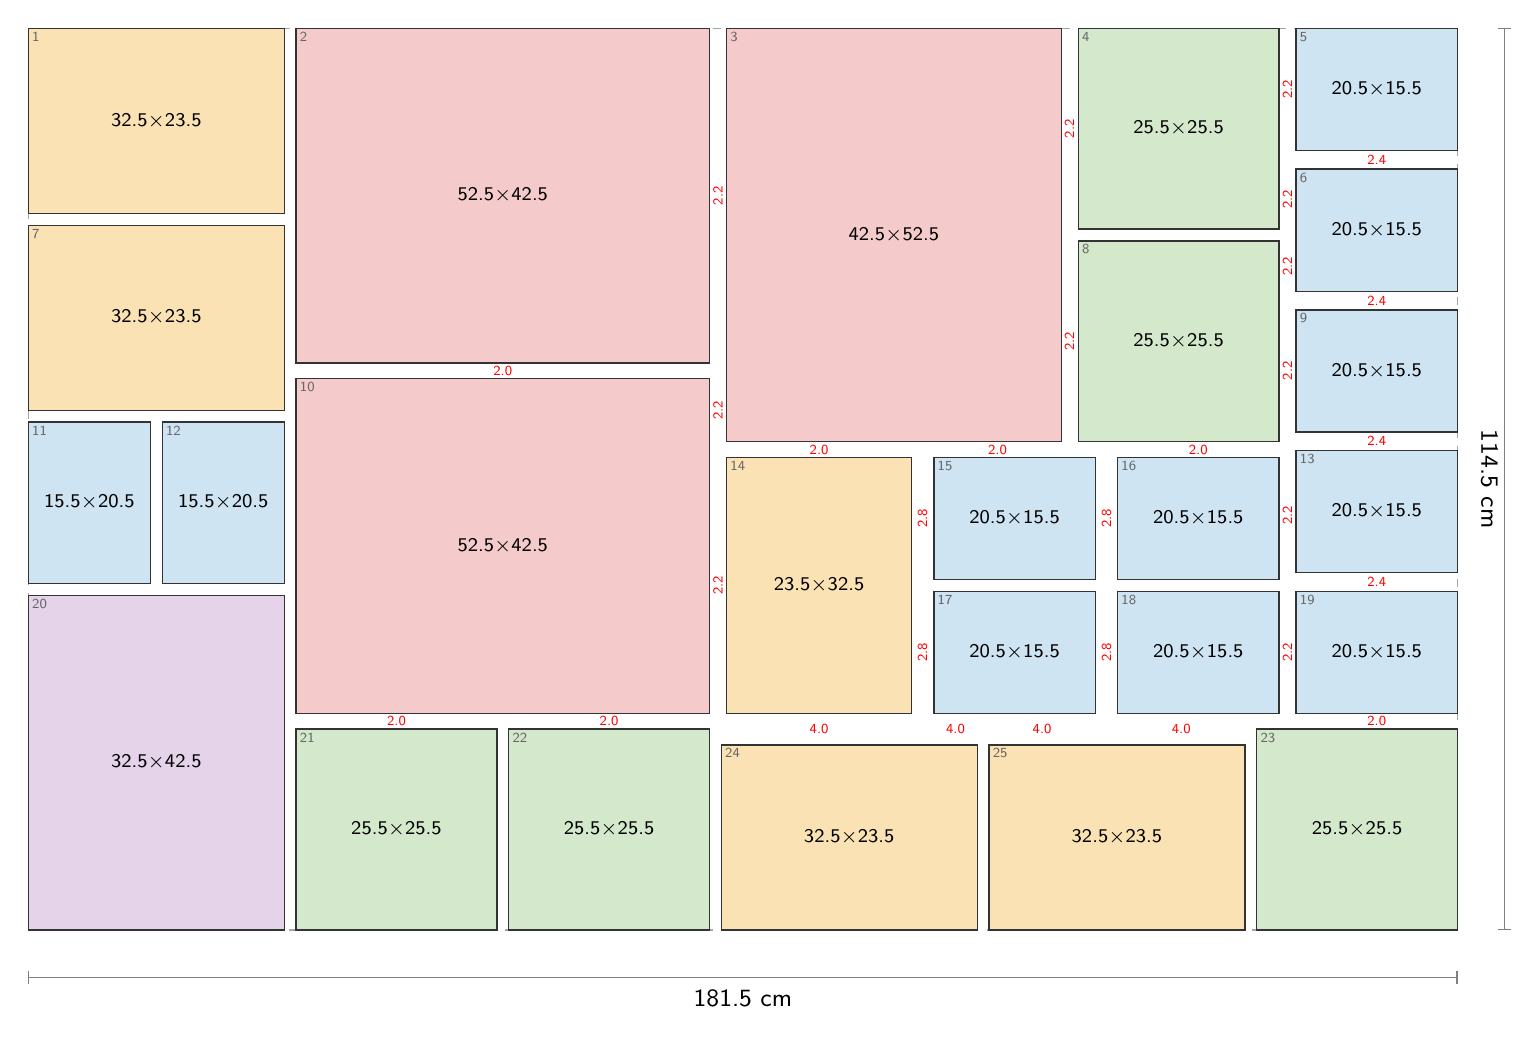
\begin{tikzpicture}[x=1mm, y=-1mm]
\draw[gray!70, dashed, line width=0.4pt] (0,0) rectangle (181.50,114.50);
\filldraw[fill=ft1, draw=black!80, line width=0.5pt] (0.00,0.00) rectangle (32.50,23.50);
\node[align=center, inner sep=0pt] at (16.25,11.75) {\scriptsize 32.5$\times$23.5};
\node[anchor=north west, inner sep=1.2pt, font=\tiny, text=black!60] at (0.00,0.00) {1};
\filldraw[fill=ft4, draw=black!80, line width=0.5pt] (34.00,0.00) rectangle (86.50,42.50);
\node[align=center, inner sep=0pt] at (60.25,21.25) {\scriptsize 52.5$\times$42.5};
\node[anchor=north west, inner sep=1.2pt, font=\tiny, text=black!60] at (34.00,0.00) {2};
\filldraw[fill=ft4, draw=black!80, line width=0.5pt] (88.67,0.00) rectangle (131.17,52.50);
\node[align=center, inner sep=0pt] at (109.92,26.25) {\scriptsize 42.5$\times$52.5};
\node[anchor=north west, inner sep=1.2pt, font=\tiny, text=black!60] at (88.67,0.00) {3};
\filldraw[fill=ft2, draw=black!80, line width=0.5pt] (133.33,0.00) rectangle (158.83,25.50);
\node[align=center, inner sep=0pt] at (146.08,12.75) {\scriptsize 25.5$\times$25.5};
\node[anchor=north west, inner sep=1.2pt, font=\tiny, text=black!60] at (133.33,0.00) {4};
\filldraw[fill=ft0, draw=black!80, line width=0.5pt] (161.00,0.00) rectangle (181.50,15.50);
\node[align=center, inner sep=0pt] at (171.25,7.75) {\scriptsize 20.5$\times$15.5};
\node[anchor=north west, inner sep=1.2pt, font=\tiny, text=black!60] at (161.00,0.00) {5};
\filldraw[fill=ft0, draw=black!80, line width=0.5pt] (161.00,17.88) rectangle (181.50,33.38);
\node[align=center, inner sep=0pt] at (171.25,25.62) {\scriptsize 20.5$\times$15.5};
\node[anchor=north west, inner sep=1.2pt, font=\tiny, text=black!60] at (161.00,17.88) {6};
\filldraw[fill=ft1, draw=black!80, line width=0.5pt] (0.00,25.00) rectangle (32.50,48.50);
\node[align=center, inner sep=0pt] at (16.25,36.75) {\scriptsize 32.5$\times$23.5};
\node[anchor=north west, inner sep=1.2pt, font=\tiny, text=black!60] at (0.00,25.00) {7};
\filldraw[fill=ft2, draw=black!80, line width=0.5pt] (133.33,27.00) rectangle (158.83,52.50);
\node[align=center, inner sep=0pt] at (146.08,39.75) {\scriptsize 25.5$\times$25.5};
\node[anchor=north west, inner sep=1.2pt, font=\tiny, text=black!60] at (133.33,27.00) {8};
\filldraw[fill=ft0, draw=black!80, line width=0.5pt] (161.00,35.75) rectangle (181.50,51.25);
\node[align=center, inner sep=0pt] at (171.25,43.50) {\scriptsize 20.5$\times$15.5};
\node[anchor=north west, inner sep=1.2pt, font=\tiny, text=black!60] at (161.00,35.75) {9};
\filldraw[fill=ft4, draw=black!80, line width=0.5pt] (34.00,44.50) rectangle (86.50,87.00);
\node[align=center, inner sep=0pt] at (60.25,65.75) {\scriptsize 52.5$\times$42.5};
\node[anchor=north west, inner sep=1.2pt, font=\tiny, text=black!60] at (34.00,44.50) {10};
\filldraw[fill=ft0, draw=black!80, line width=0.5pt] (0.00,50.00) rectangle (15.50,70.50);
\node[align=center, inner sep=0pt] at (7.75,60.25) {\scriptsize 15.5$\times$20.5};
\node[anchor=north west, inner sep=1.2pt, font=\tiny, text=black!60] at (0.00,50.00) {11};
\filldraw[fill=ft0, draw=black!80, line width=0.5pt] (17.00,50.00) rectangle (32.50,70.50);
\node[align=center, inner sep=0pt] at (24.75,60.25) {\scriptsize 15.5$\times$20.5};
\node[anchor=north west, inner sep=1.2pt, font=\tiny, text=black!60] at (17.00,50.00) {12};
\filldraw[fill=ft0, draw=black!80, line width=0.5pt] (161.00,53.62) rectangle (181.50,69.12);
\node[align=center, inner sep=0pt] at (171.25,61.38) {\scriptsize 20.5$\times$15.5};
\node[anchor=north west, inner sep=1.2pt, font=\tiny, text=black!60] at (161.00,53.62) {13};
\filldraw[fill=ft1, draw=black!80, line width=0.5pt] (88.67,54.50) rectangle (112.17,87.00);
\node[align=center, inner sep=0pt] at (100.42,70.75) {\scriptsize 23.5$\times$32.5};
\node[anchor=north west, inner sep=1.2pt, font=\tiny, text=black!60] at (88.67,54.50) {14};
\filldraw[fill=ft0, draw=black!80, line width=0.5pt] (115.00,54.50) rectangle (135.50,70.00);
\node[align=center, inner sep=0pt] at (125.25,62.25) {\scriptsize 20.5$\times$15.5};
\node[anchor=north west, inner sep=1.2pt, font=\tiny, text=black!60] at (115.00,54.50) {15};
\filldraw[fill=ft0, draw=black!80, line width=0.5pt] (138.33,54.50) rectangle (158.83,70.00);
\node[align=center, inner sep=0pt] at (148.58,62.25) {\scriptsize 20.5$\times$15.5};
\node[anchor=north west, inner sep=1.2pt, font=\tiny, text=black!60] at (138.33,54.50) {16};
\filldraw[fill=ft0, draw=black!80, line width=0.5pt] (115.00,71.50) rectangle (135.50,87.00);
\node[align=center, inner sep=0pt] at (125.25,79.25) {\scriptsize 20.5$\times$15.5};
\node[anchor=north west, inner sep=1.2pt, font=\tiny, text=black!60] at (115.00,71.50) {17};
\filldraw[fill=ft0, draw=black!80, line width=0.5pt] (138.33,71.50) rectangle (158.83,87.00);
\node[align=center, inner sep=0pt] at (148.58,79.25) {\scriptsize 20.5$\times$15.5};
\node[anchor=north west, inner sep=1.2pt, font=\tiny, text=black!60] at (138.33,71.50) {18};
\filldraw[fill=ft0, draw=black!80, line width=0.5pt] (161.00,71.50) rectangle (181.50,87.00);
\node[align=center, inner sep=0pt] at (171.25,79.25) {\scriptsize 20.5$\times$15.5};
\node[anchor=north west, inner sep=1.2pt, font=\tiny, text=black!60] at (161.00,71.50) {19};
\filldraw[fill=ft3, draw=black!80, line width=0.5pt] (0.00,72.00) rectangle (32.50,114.50);
\node[align=center, inner sep=0pt] at (16.25,93.25) {\scriptsize 32.5$\times$42.5};
\node[anchor=north west, inner sep=1.2pt, font=\tiny, text=black!60] at (0.00,72.00) {20};
\filldraw[fill=ft2, draw=black!80, line width=0.5pt] (34.00,89.00) rectangle (59.50,114.50);
\node[align=center, inner sep=0pt] at (46.75,101.75) {\scriptsize 25.5$\times$25.5};
\node[anchor=north west, inner sep=1.2pt, font=\tiny, text=black!60] at (34.00,89.00) {21};
\filldraw[fill=ft2, draw=black!80, line width=0.5pt] (61.00,89.00) rectangle (86.50,114.50);
\node[align=center, inner sep=0pt] at (73.75,101.75) {\scriptsize 25.5$\times$25.5};
\node[anchor=north west, inner sep=1.2pt, font=\tiny, text=black!60] at (61.00,89.00) {22};
\filldraw[fill=ft2, draw=black!80, line width=0.5pt] (156.00,89.00) rectangle (181.50,114.50);
\node[align=center, inner sep=0pt] at (168.75,101.75) {\scriptsize 25.5$\times$25.5};
\node[anchor=north west, inner sep=1.2pt, font=\tiny, text=black!60] at (156.00,89.00) {23};
\filldraw[fill=ft1, draw=black!80, line width=0.5pt] (88.00,91.00) rectangle (120.50,114.50);
\node[align=center, inner sep=0pt] at (104.25,102.75) {\scriptsize 32.5$\times$23.5};
\node[anchor=north west, inner sep=1.2pt, font=\tiny, text=black!60] at (88.00,91.00) {24};
\filldraw[fill=ft1, draw=black!80, line width=0.5pt] (122.00,91.00) rectangle (154.50,114.50);
\node[align=center, inner sep=0pt] at (138.25,102.75) {\scriptsize 32.5$\times$23.5};
\node[anchor=north west, inner sep=1.2pt, font=\tiny, text=black!60] at (122.00,91.00) {25};
\node[font=\tiny, text=red, fill=white, inner sep=0.3pt, rotate=90] at (87.58,21.25) {2.2};
\node[font=\tiny, text=red, fill=white, inner sep=0.3pt] at (60.25,43.50) {2.0};
\node[font=\tiny, text=red, fill=white, inner sep=0.3pt, rotate=90] at (132.25,12.75) {2.2};
\node[font=\tiny, text=red, fill=white, inner sep=0.3pt, rotate=90] at (132.25,39.75) {2.2};
\node[font=\tiny, text=red, fill=white, inner sep=0.3pt] at (100.42,53.50) {2.0};
\node[font=\tiny, text=red, fill=white, inner sep=0.3pt] at (123.08,53.50) {2.0};
\node[font=\tiny, text=red, fill=white, inner sep=0.3pt, rotate=90] at (159.92,7.75) {2.2};
\node[font=\tiny, text=red, fill=white, inner sep=0.3pt, rotate=90] at (159.92,21.69) {2.2};
\node[font=\tiny, text=red, fill=white, inner sep=0.3pt] at (171.25,16.69) {2.4};
\node[font=\tiny, text=red, fill=white, inner sep=0.3pt] at (171.25,34.56) {2.4};
\node[font=\tiny, text=red, fill=white, inner sep=0.3pt, rotate=90] at (159.92,30.19) {2.2};
\node[font=\tiny, text=red, fill=white, inner sep=0.3pt, rotate=90] at (159.92,43.50) {2.2};
\node[font=\tiny, text=red, fill=white, inner sep=0.3pt] at (148.58,53.50) {2.0};
\node[font=\tiny, text=red, fill=white, inner sep=0.3pt] at (171.25,52.44) {2.4};
\node[font=\tiny, text=red, fill=white, inner sep=0.3pt, rotate=90] at (87.58,48.50) {2.2};
\node[font=\tiny, text=red, fill=white, inner sep=0.3pt, rotate=90] at (87.58,70.75) {2.2};
\node[font=\tiny, text=red, fill=white, inner sep=0.3pt] at (46.75,88.00) {2.0};
\node[font=\tiny, text=red, fill=white, inner sep=0.3pt] at (73.75,88.00) {2.0};
\node[font=\tiny, text=red, fill=white, inner sep=0.3pt] at (171.25,70.31) {2.4};
\node[font=\tiny, text=red, fill=white, inner sep=0.3pt, rotate=90] at (113.58,62.25) {2.8};
\node[font=\tiny, text=red, fill=white, inner sep=0.3pt, rotate=90] at (113.58,79.25) {2.8};
\node[font=\tiny, text=red, fill=white, inner sep=0.3pt] at (100.42,89.00) {4.0};
\node[font=\tiny, text=red, fill=white, inner sep=0.3pt, rotate=90] at (136.92,62.25) {2.8};
\node[font=\tiny, text=red, fill=white, inner sep=0.3pt, rotate=90] at (159.92,61.81) {2.2};
\node[font=\tiny, text=red, fill=white, inner sep=0.3pt, rotate=90] at (136.92,79.25) {2.8};
\node[font=\tiny, text=red, fill=white, inner sep=0.3pt] at (117.75,89.00) {4.0};
\node[font=\tiny, text=red, fill=white, inner sep=0.3pt] at (128.75,89.00) {4.0};
\node[font=\tiny, text=red, fill=white, inner sep=0.3pt, rotate=90] at (159.92,79.25) {2.2};
\node[font=\tiny, text=red, fill=white, inner sep=0.3pt] at (146.42,89.00) {4.0};
\node[font=\tiny, text=red, fill=white, inner sep=0.3pt] at (171.25,88.00) {2.0};
\draw[Bar-Bar, gray] (0,120.50) -- (181.50,120.50) node[midway, below=1pt, font=\small, text=black] {181.5 cm};
\draw[Bar-Bar, gray] (187.50,0) -- (187.50,114.50) node[midway, right=1pt, font=\small, text=black, rotate=-90, anchor=north] {114.5 cm};
\end{tikzpicture}\\[4pt]
{\scriptsize Scale 1:10 (1 mm = 1 cm). Red numbers mark gaps that deviate from the nominal gap by more than 0.25 cm. Small grey numbers index the coordinate table.}
\end{minipage}\hfill
\begin{minipage}[t]{0.25\textwidth}\vspace{0pt}
\small
\begin{tabular}{@{}l l@{}}
\toprule
Outer size & 181.5 $\times$ 114.5 cm \\
Nominal gap & 1.5 cm \\
Actual gaps & 1.5 -- 4.0 cm \\
Max.\ deviation & 2.5 cm \\
Mean deviation & 0.62 cm \\
Border notches & none \\
Corners filled & 4 / 4 \\
Frames used & 25 of 28 \\
\bottomrule
\end{tabular}

\vspace{8pt}
\scriptsize
\begin{tabular}{@{}c l l r r@{}}
\toprule
 & outer w $\times$ h (cm) & & used & have \\
\midrule
\tikz[baseline=-0.6ex]\fill[ft0,draw=black!60] (0,0) rectangle (1.2ex,1.2ex); & 20.5$\times$15.5 & L & 9 & 9 \\
\tikz[baseline=-0.6ex]\fill[ft0,draw=black!60] (0,0) rectangle (1.2ex,1.2ex); & 15.5$\times$20.5 & P & 2 & 2 \\
\tikz[baseline=-0.6ex]\fill[ft3,draw=black!60] (0,0) rectangle (1.2ex,1.2ex); & 32.5$\times$42.5 & P & 1 & 2 \\
\tikz[baseline=-0.6ex]\fill[ft3,draw=black!60] (0,0) rectangle (1.2ex,1.2ex); & 42.5$\times$32.5 & L & 0 & 1 \\
\tikz[baseline=-0.6ex]\fill[ft1,draw=black!60] (0,0) rectangle (1.2ex,1.2ex); & 32.5$\times$23.5 & L & 4 & 5 \\
\tikz[baseline=-0.6ex]\fill[ft1,draw=black!60] (0,0) rectangle (1.2ex,1.2ex); & 23.5$\times$32.5 & P & 1 & 1 \\
\tikz[baseline=-0.6ex]\fill[ft2,draw=black!60] (0,0) rectangle (1.2ex,1.2ex); & 25.5$\times$25.5 &  & 5 & 5 \\
\tikz[baseline=-0.6ex]\fill[ft4,draw=black!60] (0,0) rectangle (1.2ex,1.2ex); & 42.5$\times$52.5 & P & 1 & 1 \\
\tikz[baseline=-0.6ex]\fill[ft4,draw=black!60] (0,0) rectangle (1.2ex,1.2ex); & 52.5$\times$42.5 & L & 2 & 2 \\
\bottomrule
\end{tabular}

\vspace{8pt}
{\bfseries Positions} (top-left corner, cm)\\[2pt]
\tiny
\begin{tabular}{@{}r l r r@{}}
\toprule
\# & frame w $\times$ h & x & y \\
\midrule
1 & 32.5 $\times$ 23.5 & 0.0 & 0.0 \\
2 & 52.5 $\times$ 42.5 & 34.0 & 0.0 \\
3 & 42.5 $\times$ 52.5 & 88.7 & 0.0 \\
4 & 25.5 $\times$ 25.5 & 133.3 & 0.0 \\
5 & 20.5 $\times$ 15.5 & 161.0 & 0.0 \\
6 & 20.5 $\times$ 15.5 & 161.0 & 17.9 \\
7 & 32.5 $\times$ 23.5 & 0.0 & 25.0 \\
8 & 25.5 $\times$ 25.5 & 133.3 & 27.0 \\
9 & 20.5 $\times$ 15.5 & 161.0 & 35.8 \\
10 & 52.5 $\times$ 42.5 & 34.0 & 44.5 \\
11 & 15.5 $\times$ 20.5 & 0.0 & 50.0 \\
12 & 15.5 $\times$ 20.5 & 17.0 & 50.0 \\
13 & 20.5 $\times$ 15.5 & 161.0 & 53.6 \\
14 & 23.5 $\times$ 32.5 & 88.7 & 54.5 \\
15 & 20.5 $\times$ 15.5 & 115.0 & 54.5 \\
16 & 20.5 $\times$ 15.5 & 138.3 & 54.5 \\
17 & 20.5 $\times$ 15.5 & 115.0 & 71.5 \\
18 & 20.5 $\times$ 15.5 & 138.3 & 71.5 \\
19 & 20.5 $\times$ 15.5 & 161.0 & 71.5 \\
20 & 32.5 $\times$ 42.5 & 0.0 & 72.0 \\
21 & 25.5 $\times$ 25.5 & 34.0 & 89.0 \\
22 & 25.5 $\times$ 25.5 & 61.0 & 89.0 \\
23 & 25.5 $\times$ 25.5 & 156.0 & 89.0 \\
24 & 32.5 $\times$ 23.5 & 88.0 & 91.0 \\
25 & 32.5 $\times$ 23.5 & 122.0 & 91.0 \\
\bottomrule
\end{tabular}
\end{minipage}
\clearpage

\begin{minipage}[t]{0.74\textwidth}\vspace{0pt}
{\LARGE\bfseries Layout 13}\hspace{1.5em}{\large 185.5 $\times$ 113.5 cm \quad gap 1.5 cm \quad 24 frames}\\[8pt]
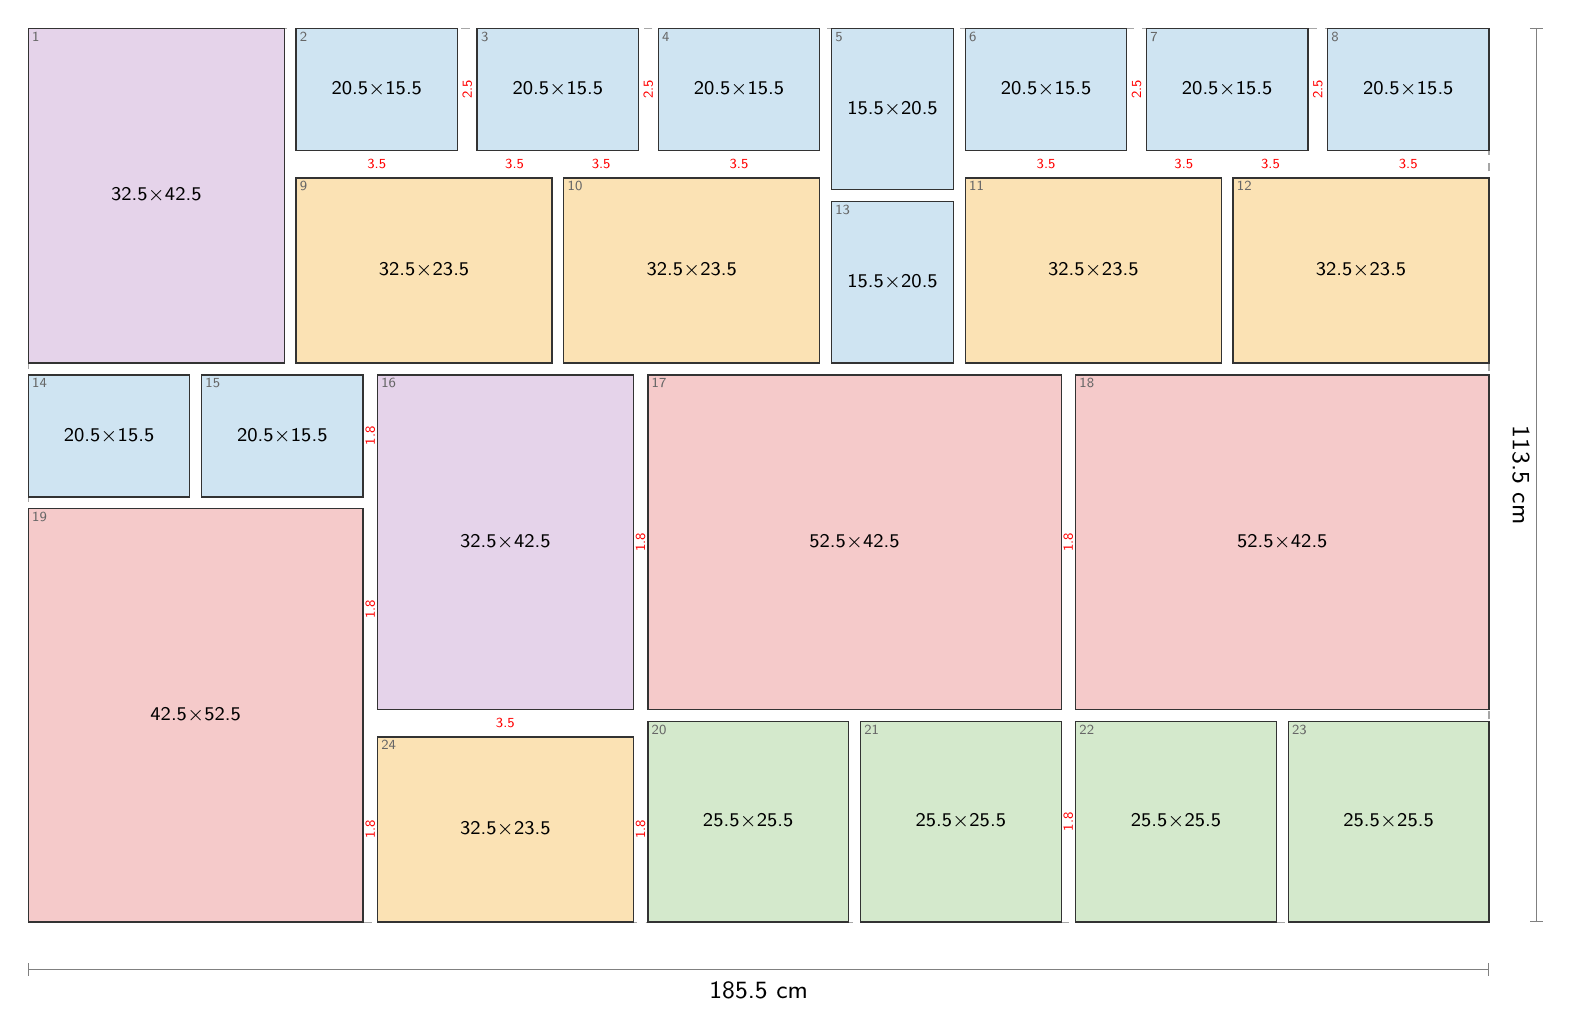
\begin{tikzpicture}[x=1mm, y=-1mm]
\draw[gray!70, dashed, line width=0.4pt] (0,0) rectangle (185.50,113.50);
\filldraw[fill=ft3, draw=black!80, line width=0.5pt] (0.00,0.00) rectangle (32.50,42.50);
\node[align=center, inner sep=0pt] at (16.25,21.25) {\scriptsize 32.5$\times$42.5};
\node[anchor=north west, inner sep=1.2pt, font=\tiny, text=black!60] at (0.00,0.00) {1};
\filldraw[fill=ft0, draw=black!80, line width=0.5pt] (34.00,0.00) rectangle (54.50,15.50);
\node[align=center, inner sep=0pt] at (44.25,7.75) {\scriptsize 20.5$\times$15.5};
\node[anchor=north west, inner sep=1.2pt, font=\tiny, text=black!60] at (34.00,0.00) {2};
\filldraw[fill=ft0, draw=black!80, line width=0.5pt] (57.00,0.00) rectangle (77.50,15.50);
\node[align=center, inner sep=0pt] at (67.25,7.75) {\scriptsize 20.5$\times$15.5};
\node[anchor=north west, inner sep=1.2pt, font=\tiny, text=black!60] at (57.00,0.00) {3};
\filldraw[fill=ft0, draw=black!80, line width=0.5pt] (80.00,0.00) rectangle (100.50,15.50);
\node[align=center, inner sep=0pt] at (90.25,7.75) {\scriptsize 20.5$\times$15.5};
\node[anchor=north west, inner sep=1.2pt, font=\tiny, text=black!60] at (80.00,0.00) {4};
\filldraw[fill=ft0, draw=black!80, line width=0.5pt] (102.00,0.00) rectangle (117.50,20.50);
\node[align=center, inner sep=0pt] at (109.75,10.25) {\scriptsize 15.5$\times$20.5};
\node[anchor=north west, inner sep=1.2pt, font=\tiny, text=black!60] at (102.00,0.00) {5};
\filldraw[fill=ft0, draw=black!80, line width=0.5pt] (119.00,0.00) rectangle (139.50,15.50);
\node[align=center, inner sep=0pt] at (129.25,7.75) {\scriptsize 20.5$\times$15.5};
\node[anchor=north west, inner sep=1.2pt, font=\tiny, text=black!60] at (119.00,0.00) {6};
\filldraw[fill=ft0, draw=black!80, line width=0.5pt] (142.00,0.00) rectangle (162.50,15.50);
\node[align=center, inner sep=0pt] at (152.25,7.75) {\scriptsize 20.5$\times$15.5};
\node[anchor=north west, inner sep=1.2pt, font=\tiny, text=black!60] at (142.00,0.00) {7};
\filldraw[fill=ft0, draw=black!80, line width=0.5pt] (165.00,0.00) rectangle (185.50,15.50);
\node[align=center, inner sep=0pt] at (175.25,7.75) {\scriptsize 20.5$\times$15.5};
\node[anchor=north west, inner sep=1.2pt, font=\tiny, text=black!60] at (165.00,0.00) {8};
\filldraw[fill=ft1, draw=black!80, line width=0.5pt] (34.00,19.00) rectangle (66.50,42.50);
\node[align=center, inner sep=0pt] at (50.25,30.75) {\scriptsize 32.5$\times$23.5};
\node[anchor=north west, inner sep=1.2pt, font=\tiny, text=black!60] at (34.00,19.00) {9};
\filldraw[fill=ft1, draw=black!80, line width=0.5pt] (68.00,19.00) rectangle (100.50,42.50);
\node[align=center, inner sep=0pt] at (84.25,30.75) {\scriptsize 32.5$\times$23.5};
\node[anchor=north west, inner sep=1.2pt, font=\tiny, text=black!60] at (68.00,19.00) {10};
\filldraw[fill=ft1, draw=black!80, line width=0.5pt] (119.00,19.00) rectangle (151.50,42.50);
\node[align=center, inner sep=0pt] at (135.25,30.75) {\scriptsize 32.5$\times$23.5};
\node[anchor=north west, inner sep=1.2pt, font=\tiny, text=black!60] at (119.00,19.00) {11};
\filldraw[fill=ft1, draw=black!80, line width=0.5pt] (153.00,19.00) rectangle (185.50,42.50);
\node[align=center, inner sep=0pt] at (169.25,30.75) {\scriptsize 32.5$\times$23.5};
\node[anchor=north west, inner sep=1.2pt, font=\tiny, text=black!60] at (153.00,19.00) {12};
\filldraw[fill=ft0, draw=black!80, line width=0.5pt] (102.00,22.00) rectangle (117.50,42.50);
\node[align=center, inner sep=0pt] at (109.75,32.25) {\scriptsize 15.5$\times$20.5};
\node[anchor=north west, inner sep=1.2pt, font=\tiny, text=black!60] at (102.00,22.00) {13};
\filldraw[fill=ft0, draw=black!80, line width=0.5pt] (0.00,44.00) rectangle (20.50,59.50);
\node[align=center, inner sep=0pt] at (10.25,51.75) {\scriptsize 20.5$\times$15.5};
\node[anchor=north west, inner sep=1.2pt, font=\tiny, text=black!60] at (0.00,44.00) {14};
\filldraw[fill=ft0, draw=black!80, line width=0.5pt] (22.00,44.00) rectangle (42.50,59.50);
\node[align=center, inner sep=0pt] at (32.25,51.75) {\scriptsize 20.5$\times$15.5};
\node[anchor=north west, inner sep=1.2pt, font=\tiny, text=black!60] at (22.00,44.00) {15};
\filldraw[fill=ft3, draw=black!80, line width=0.5pt] (44.33,44.00) rectangle (76.83,86.50);
\node[align=center, inner sep=0pt] at (60.58,65.25) {\scriptsize 32.5$\times$42.5};
\node[anchor=north west, inner sep=1.2pt, font=\tiny, text=black!60] at (44.33,44.00) {16};
\filldraw[fill=ft4, draw=black!80, line width=0.5pt] (78.67,44.00) rectangle (131.17,86.50);
\node[align=center, inner sep=0pt] at (104.92,65.25) {\scriptsize 52.5$\times$42.5};
\node[anchor=north west, inner sep=1.2pt, font=\tiny, text=black!60] at (78.67,44.00) {17};
\filldraw[fill=ft4, draw=black!80, line width=0.5pt] (133.00,44.00) rectangle (185.50,86.50);
\node[align=center, inner sep=0pt] at (159.25,65.25) {\scriptsize 52.5$\times$42.5};
\node[anchor=north west, inner sep=1.2pt, font=\tiny, text=black!60] at (133.00,44.00) {18};
\filldraw[fill=ft4, draw=black!80, line width=0.5pt] (0.00,61.00) rectangle (42.50,113.50);
\node[align=center, inner sep=0pt] at (21.25,87.25) {\scriptsize 42.5$\times$52.5};
\node[anchor=north west, inner sep=1.2pt, font=\tiny, text=black!60] at (0.00,61.00) {19};
\filldraw[fill=ft2, draw=black!80, line width=0.5pt] (78.67,88.00) rectangle (104.17,113.50);
\node[align=center, inner sep=0pt] at (91.42,100.75) {\scriptsize 25.5$\times$25.5};
\node[anchor=north west, inner sep=1.2pt, font=\tiny, text=black!60] at (78.67,88.00) {20};
\filldraw[fill=ft2, draw=black!80, line width=0.5pt] (105.67,88.00) rectangle (131.17,113.50);
\node[align=center, inner sep=0pt] at (118.42,100.75) {\scriptsize 25.5$\times$25.5};
\node[anchor=north west, inner sep=1.2pt, font=\tiny, text=black!60] at (105.67,88.00) {21};
\filldraw[fill=ft2, draw=black!80, line width=0.5pt] (133.00,88.00) rectangle (158.50,113.50);
\node[align=center, inner sep=0pt] at (145.75,100.75) {\scriptsize 25.5$\times$25.5};
\node[anchor=north west, inner sep=1.2pt, font=\tiny, text=black!60] at (133.00,88.00) {22};
\filldraw[fill=ft2, draw=black!80, line width=0.5pt] (160.00,88.00) rectangle (185.50,113.50);
\node[align=center, inner sep=0pt] at (172.75,100.75) {\scriptsize 25.5$\times$25.5};
\node[anchor=north west, inner sep=1.2pt, font=\tiny, text=black!60] at (160.00,88.00) {23};
\filldraw[fill=ft1, draw=black!80, line width=0.5pt] (44.33,90.00) rectangle (76.83,113.50);
\node[align=center, inner sep=0pt] at (60.58,101.75) {\scriptsize 32.5$\times$23.5};
\node[anchor=north west, inner sep=1.2pt, font=\tiny, text=black!60] at (44.33,90.00) {24};
\node[font=\tiny, text=red, fill=white, inner sep=0.3pt, rotate=90] at (55.75,7.75) {2.5};
\node[font=\tiny, text=red, fill=white, inner sep=0.3pt] at (44.25,17.25) {3.5};
\node[font=\tiny, text=red, fill=white, inner sep=0.3pt, rotate=90] at (78.75,7.75) {2.5};
\node[font=\tiny, text=red, fill=white, inner sep=0.3pt] at (61.75,17.25) {3.5};
\node[font=\tiny, text=red, fill=white, inner sep=0.3pt] at (72.75,17.25) {3.5};
\node[font=\tiny, text=red, fill=white, inner sep=0.3pt] at (90.25,17.25) {3.5};
\node[font=\tiny, text=red, fill=white, inner sep=0.3pt, rotate=90] at (140.75,7.75) {2.5};
\node[font=\tiny, text=red, fill=white, inner sep=0.3pt] at (129.25,17.25) {3.5};
\node[font=\tiny, text=red, fill=white, inner sep=0.3pt, rotate=90] at (163.75,7.75) {2.5};
\node[font=\tiny, text=red, fill=white, inner sep=0.3pt] at (146.75,17.25) {3.5};
\node[font=\tiny, text=red, fill=white, inner sep=0.3pt] at (157.75,17.25) {3.5};
\node[font=\tiny, text=red, fill=white, inner sep=0.3pt] at (175.25,17.25) {3.5};
\node[font=\tiny, text=red, fill=white, inner sep=0.3pt, rotate=90] at (43.42,51.75) {1.8};
\node[font=\tiny, text=red, fill=white, inner sep=0.3pt, rotate=90] at (77.75,65.25) {1.8};
\node[font=\tiny, text=red, fill=white, inner sep=0.3pt] at (60.58,88.25) {3.5};
\node[font=\tiny, text=red, fill=white, inner sep=0.3pt, rotate=90] at (132.08,65.25) {1.8};
\node[font=\tiny, text=red, fill=white, inner sep=0.3pt, rotate=90] at (43.42,73.75) {1.8};
\node[font=\tiny, text=red, fill=white, inner sep=0.3pt, rotate=90] at (43.42,101.75) {1.8};
\node[font=\tiny, text=red, fill=white, inner sep=0.3pt, rotate=90] at (132.08,100.75) {1.8};
\node[font=\tiny, text=red, fill=white, inner sep=0.3pt, rotate=90] at (77.75,101.75) {1.8};
\draw[Bar-Bar, gray] (0,119.50) -- (185.50,119.50) node[midway, below=1pt, font=\small, text=black] {185.5 cm};
\draw[Bar-Bar, gray] (191.50,0) -- (191.50,113.50) node[midway, right=1pt, font=\small, text=black, rotate=-90, anchor=north] {113.5 cm};
\end{tikzpicture}\\[4pt]
{\scriptsize Scale 1:10 (1 mm = 1 cm). Red numbers mark gaps that deviate from the nominal gap by more than 0.25 cm. Small grey numbers index the coordinate table.}
\end{minipage}\hfill
\begin{minipage}[t]{0.25\textwidth}\vspace{0pt}
\small
\begin{tabular}{@{}l l@{}}
\toprule
Outer size & 185.5 $\times$ 113.5 cm \\
Nominal gap & 1.5 cm \\
Actual gaps & 1.5 -- 3.5 cm \\
Max.\ deviation & 2.0 cm \\
Mean deviation & 0.51 cm \\
Border notches & right 4 cm \\
Corners filled & 4 / 4 \\
Frames used & 24 of 28 \\
\bottomrule
\end{tabular}

\vspace{8pt}
\scriptsize
\begin{tabular}{@{}c l l r r@{}}
\toprule
 & outer w $\times$ h (cm) & & used & have \\
\midrule
\tikz[baseline=-0.6ex]\fill[ft0,draw=black!60] (0,0) rectangle (1.2ex,1.2ex); & 20.5$\times$15.5 & L & 8 & 9 \\
\tikz[baseline=-0.6ex]\fill[ft0,draw=black!60] (0,0) rectangle (1.2ex,1.2ex); & 15.5$\times$20.5 & P & 2 & 2 \\
\tikz[baseline=-0.6ex]\fill[ft3,draw=black!60] (0,0) rectangle (1.2ex,1.2ex); & 32.5$\times$42.5 & P & 2 & 2 \\
\tikz[baseline=-0.6ex]\fill[ft3,draw=black!60] (0,0) rectangle (1.2ex,1.2ex); & 42.5$\times$32.5 & L & 0 & 1 \\
\tikz[baseline=-0.6ex]\fill[ft1,draw=black!60] (0,0) rectangle (1.2ex,1.2ex); & 32.5$\times$23.5 & L & 5 & 5 \\
\tikz[baseline=-0.6ex]\fill[ft1,draw=black!60] (0,0) rectangle (1.2ex,1.2ex); & 23.5$\times$32.5 & P & 0 & 1 \\
\tikz[baseline=-0.6ex]\fill[ft2,draw=black!60] (0,0) rectangle (1.2ex,1.2ex); & 25.5$\times$25.5 &  & 4 & 5 \\
\tikz[baseline=-0.6ex]\fill[ft4,draw=black!60] (0,0) rectangle (1.2ex,1.2ex); & 42.5$\times$52.5 & P & 1 & 1 \\
\tikz[baseline=-0.6ex]\fill[ft4,draw=black!60] (0,0) rectangle (1.2ex,1.2ex); & 52.5$\times$42.5 & L & 2 & 2 \\
\bottomrule
\end{tabular}

\vspace{8pt}
{\bfseries Positions} (top-left corner, cm)\\[2pt]
\tiny
\begin{tabular}{@{}r l r r@{}}
\toprule
\# & frame w $\times$ h & x & y \\
\midrule
1 & 32.5 $\times$ 42.5 & 0.0 & 0.0 \\
2 & 20.5 $\times$ 15.5 & 34.0 & 0.0 \\
3 & 20.5 $\times$ 15.5 & 57.0 & 0.0 \\
4 & 20.5 $\times$ 15.5 & 80.0 & 0.0 \\
5 & 15.5 $\times$ 20.5 & 102.0 & 0.0 \\
6 & 20.5 $\times$ 15.5 & 119.0 & 0.0 \\
7 & 20.5 $\times$ 15.5 & 142.0 & 0.0 \\
8 & 20.5 $\times$ 15.5 & 165.0 & 0.0 \\
9 & 32.5 $\times$ 23.5 & 34.0 & 19.0 \\
10 & 32.5 $\times$ 23.5 & 68.0 & 19.0 \\
11 & 32.5 $\times$ 23.5 & 119.0 & 19.0 \\
12 & 32.5 $\times$ 23.5 & 153.0 & 19.0 \\
13 & 15.5 $\times$ 20.5 & 102.0 & 22.0 \\
14 & 20.5 $\times$ 15.5 & 0.0 & 44.0 \\
15 & 20.5 $\times$ 15.5 & 22.0 & 44.0 \\
16 & 32.5 $\times$ 42.5 & 44.3 & 44.0 \\
17 & 52.5 $\times$ 42.5 & 78.7 & 44.0 \\
18 & 52.5 $\times$ 42.5 & 133.0 & 44.0 \\
19 & 42.5 $\times$ 52.5 & 0.0 & 61.0 \\
20 & 25.5 $\times$ 25.5 & 78.7 & 88.0 \\
21 & 25.5 $\times$ 25.5 & 105.7 & 88.0 \\
22 & 25.5 $\times$ 25.5 & 133.0 & 88.0 \\
23 & 25.5 $\times$ 25.5 & 160.0 & 88.0 \\
24 & 32.5 $\times$ 23.5 & 44.3 & 90.0 \\
\bottomrule
\end{tabular}
\end{minipage}
\clearpage

\begin{minipage}[t]{0.74\textwidth}\vspace{0pt}
{\LARGE\bfseries Layout 14}\hspace{1.5em}{\large 172.5 $\times$ 115.5 cm \quad gap 2.5 cm \quad 24 frames}\\[8pt]
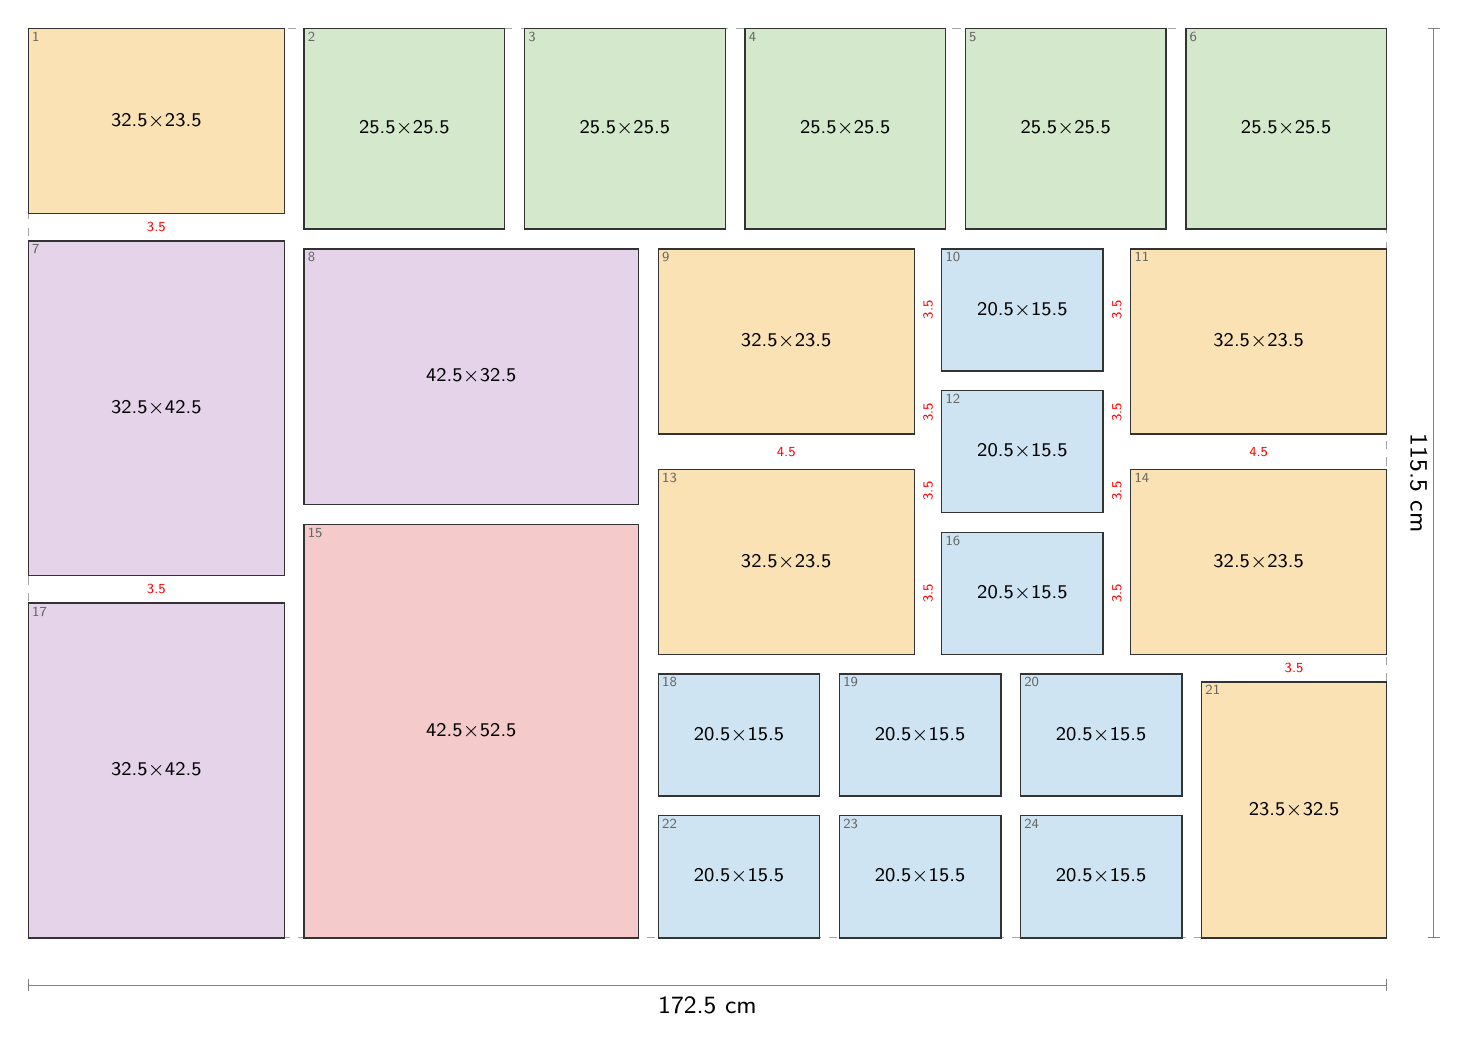
\begin{tikzpicture}[x=1mm, y=-1mm]
\draw[gray!70, dashed, line width=0.4pt] (0,0) rectangle (172.50,115.50);
\filldraw[fill=ft1, draw=black!80, line width=0.5pt] (0.00,0.00) rectangle (32.50,23.50);
\node[align=center, inner sep=0pt] at (16.25,11.75) {\scriptsize 32.5$\times$23.5};
\node[anchor=north west, inner sep=1.2pt, font=\tiny, text=black!60] at (0.00,0.00) {1};
\filldraw[fill=ft2, draw=black!80, line width=0.5pt] (35.00,0.00) rectangle (60.50,25.50);
\node[align=center, inner sep=0pt] at (47.75,12.75) {\scriptsize 25.5$\times$25.5};
\node[anchor=north west, inner sep=1.2pt, font=\tiny, text=black!60] at (35.00,0.00) {2};
\filldraw[fill=ft2, draw=black!80, line width=0.5pt] (63.00,0.00) rectangle (88.50,25.50);
\node[align=center, inner sep=0pt] at (75.75,12.75) {\scriptsize 25.5$\times$25.5};
\node[anchor=north west, inner sep=1.2pt, font=\tiny, text=black!60] at (63.00,0.00) {3};
\filldraw[fill=ft2, draw=black!80, line width=0.5pt] (91.00,0.00) rectangle (116.50,25.50);
\node[align=center, inner sep=0pt] at (103.75,12.75) {\scriptsize 25.5$\times$25.5};
\node[anchor=north west, inner sep=1.2pt, font=\tiny, text=black!60] at (91.00,0.00) {4};
\filldraw[fill=ft2, draw=black!80, line width=0.5pt] (119.00,0.00) rectangle (144.50,25.50);
\node[align=center, inner sep=0pt] at (131.75,12.75) {\scriptsize 25.5$\times$25.5};
\node[anchor=north west, inner sep=1.2pt, font=\tiny, text=black!60] at (119.00,0.00) {5};
\filldraw[fill=ft2, draw=black!80, line width=0.5pt] (147.00,0.00) rectangle (172.50,25.50);
\node[align=center, inner sep=0pt] at (159.75,12.75) {\scriptsize 25.5$\times$25.5};
\node[anchor=north west, inner sep=1.2pt, font=\tiny, text=black!60] at (147.00,0.00) {6};
\filldraw[fill=ft3, draw=black!80, line width=0.5pt] (0.00,27.00) rectangle (32.50,69.50);
\node[align=center, inner sep=0pt] at (16.25,48.25) {\scriptsize 32.5$\times$42.5};
\node[anchor=north west, inner sep=1.2pt, font=\tiny, text=black!60] at (0.00,27.00) {7};
\filldraw[fill=ft3, draw=black!80, line width=0.5pt] (35.00,28.00) rectangle (77.50,60.50);
\node[align=center, inner sep=0pt] at (56.25,44.25) {\scriptsize 42.5$\times$32.5};
\node[anchor=north west, inner sep=1.2pt, font=\tiny, text=black!60] at (35.00,28.00) {8};
\filldraw[fill=ft1, draw=black!80, line width=0.5pt] (80.00,28.00) rectangle (112.50,51.50);
\node[align=center, inner sep=0pt] at (96.25,39.75) {\scriptsize 32.5$\times$23.5};
\node[anchor=north west, inner sep=1.2pt, font=\tiny, text=black!60] at (80.00,28.00) {9};
\filldraw[fill=ft0, draw=black!80, line width=0.5pt] (116.00,28.00) rectangle (136.50,43.50);
\node[align=center, inner sep=0pt] at (126.25,35.75) {\scriptsize 20.5$\times$15.5};
\node[anchor=north west, inner sep=1.2pt, font=\tiny, text=black!60] at (116.00,28.00) {10};
\filldraw[fill=ft1, draw=black!80, line width=0.5pt] (140.00,28.00) rectangle (172.50,51.50);
\node[align=center, inner sep=0pt] at (156.25,39.75) {\scriptsize 32.5$\times$23.5};
\node[anchor=north west, inner sep=1.2pt, font=\tiny, text=black!60] at (140.00,28.00) {11};
\filldraw[fill=ft0, draw=black!80, line width=0.5pt] (116.00,46.00) rectangle (136.50,61.50);
\node[align=center, inner sep=0pt] at (126.25,53.75) {\scriptsize 20.5$\times$15.5};
\node[anchor=north west, inner sep=1.2pt, font=\tiny, text=black!60] at (116.00,46.00) {12};
\filldraw[fill=ft1, draw=black!80, line width=0.5pt] (80.00,56.00) rectangle (112.50,79.50);
\node[align=center, inner sep=0pt] at (96.25,67.75) {\scriptsize 32.5$\times$23.5};
\node[anchor=north west, inner sep=1.2pt, font=\tiny, text=black!60] at (80.00,56.00) {13};
\filldraw[fill=ft1, draw=black!80, line width=0.5pt] (140.00,56.00) rectangle (172.50,79.50);
\node[align=center, inner sep=0pt] at (156.25,67.75) {\scriptsize 32.5$\times$23.5};
\node[anchor=north west, inner sep=1.2pt, font=\tiny, text=black!60] at (140.00,56.00) {14};
\filldraw[fill=ft4, draw=black!80, line width=0.5pt] (35.00,63.00) rectangle (77.50,115.50);
\node[align=center, inner sep=0pt] at (56.25,89.25) {\scriptsize 42.5$\times$52.5};
\node[anchor=north west, inner sep=1.2pt, font=\tiny, text=black!60] at (35.00,63.00) {15};
\filldraw[fill=ft0, draw=black!80, line width=0.5pt] (116.00,64.00) rectangle (136.50,79.50);
\node[align=center, inner sep=0pt] at (126.25,71.75) {\scriptsize 20.5$\times$15.5};
\node[anchor=north west, inner sep=1.2pt, font=\tiny, text=black!60] at (116.00,64.00) {16};
\filldraw[fill=ft3, draw=black!80, line width=0.5pt] (0.00,73.00) rectangle (32.50,115.50);
\node[align=center, inner sep=0pt] at (16.25,94.25) {\scriptsize 32.5$\times$42.5};
\node[anchor=north west, inner sep=1.2pt, font=\tiny, text=black!60] at (0.00,73.00) {17};
\filldraw[fill=ft0, draw=black!80, line width=0.5pt] (80.00,82.00) rectangle (100.50,97.50);
\node[align=center, inner sep=0pt] at (90.25,89.75) {\scriptsize 20.5$\times$15.5};
\node[anchor=north west, inner sep=1.2pt, font=\tiny, text=black!60] at (80.00,82.00) {18};
\filldraw[fill=ft0, draw=black!80, line width=0.5pt] (103.00,82.00) rectangle (123.50,97.50);
\node[align=center, inner sep=0pt] at (113.25,89.75) {\scriptsize 20.5$\times$15.5};
\node[anchor=north west, inner sep=1.2pt, font=\tiny, text=black!60] at (103.00,82.00) {19};
\filldraw[fill=ft0, draw=black!80, line width=0.5pt] (126.00,82.00) rectangle (146.50,97.50);
\node[align=center, inner sep=0pt] at (136.25,89.75) {\scriptsize 20.5$\times$15.5};
\node[anchor=north west, inner sep=1.2pt, font=\tiny, text=black!60] at (126.00,82.00) {20};
\filldraw[fill=ft1, draw=black!80, line width=0.5pt] (149.00,83.00) rectangle (172.50,115.50);
\node[align=center, inner sep=0pt] at (160.75,99.25) {\scriptsize 23.5$\times$32.5};
\node[anchor=north west, inner sep=1.2pt, font=\tiny, text=black!60] at (149.00,83.00) {21};
\filldraw[fill=ft0, draw=black!80, line width=0.5pt] (80.00,100.00) rectangle (100.50,115.50);
\node[align=center, inner sep=0pt] at (90.25,107.75) {\scriptsize 20.5$\times$15.5};
\node[anchor=north west, inner sep=1.2pt, font=\tiny, text=black!60] at (80.00,100.00) {22};
\filldraw[fill=ft0, draw=black!80, line width=0.5pt] (103.00,100.00) rectangle (123.50,115.50);
\node[align=center, inner sep=0pt] at (113.25,107.75) {\scriptsize 20.5$\times$15.5};
\node[anchor=north west, inner sep=1.2pt, font=\tiny, text=black!60] at (103.00,100.00) {23};
\filldraw[fill=ft0, draw=black!80, line width=0.5pt] (126.00,100.00) rectangle (146.50,115.50);
\node[align=center, inner sep=0pt] at (136.25,107.75) {\scriptsize 20.5$\times$15.5};
\node[anchor=north west, inner sep=1.2pt, font=\tiny, text=black!60] at (126.00,100.00) {24};
\node[font=\tiny, text=red, fill=white, inner sep=0.3pt] at (16.25,25.25) {3.5};
\node[font=\tiny, text=red, fill=white, inner sep=0.3pt] at (16.25,71.25) {3.5};
\node[font=\tiny, text=red, fill=white, inner sep=0.3pt, rotate=90] at (114.25,35.75) {3.5};
\node[font=\tiny, text=red, fill=white, inner sep=0.3pt, rotate=90] at (114.25,48.75) {3.5};
\node[font=\tiny, text=red, fill=white, inner sep=0.3pt] at (96.25,53.75) {4.5};
\node[font=\tiny, text=red, fill=white, inner sep=0.3pt, rotate=90] at (138.25,35.75) {3.5};
\node[font=\tiny, text=red, fill=white, inner sep=0.3pt] at (156.25,53.75) {4.5};
\node[font=\tiny, text=red, fill=white, inner sep=0.3pt, rotate=90] at (138.25,48.75) {3.5};
\node[font=\tiny, text=red, fill=white, inner sep=0.3pt, rotate=90] at (138.25,58.75) {3.5};
\node[font=\tiny, text=red, fill=white, inner sep=0.3pt, rotate=90] at (114.25,58.75) {3.5};
\node[font=\tiny, text=red, fill=white, inner sep=0.3pt, rotate=90] at (114.25,71.75) {3.5};
\node[font=\tiny, text=red, fill=white, inner sep=0.3pt] at (160.75,81.25) {3.5};
\node[font=\tiny, text=red, fill=white, inner sep=0.3pt, rotate=90] at (138.25,71.75) {3.5};
\draw[Bar-Bar, gray] (0,121.50) -- (172.50,121.50) node[midway, below=1pt, font=\small, text=black] {172.5 cm};
\draw[Bar-Bar, gray] (178.50,0) -- (178.50,115.50) node[midway, right=1pt, font=\small, text=black, rotate=-90, anchor=north] {115.5 cm};
\end{tikzpicture}\\[4pt]
{\scriptsize Scale 1:10 (1 mm = 1 cm). Red numbers mark gaps that deviate from the nominal gap by more than 0.25 cm. Small grey numbers index the coordinate table.}
\end{minipage}\hfill
\begin{minipage}[t]{0.25\textwidth}\vspace{0pt}
\small
\begin{tabular}{@{}l l@{}}
\toprule
Outer size & 172.5 $\times$ 115.5 cm \\
Nominal gap & 2.5 cm \\
Actual gaps & 2.5 -- 4.5 cm \\
Max.\ deviation & 2.0 cm \\
Mean deviation & 0.31 cm \\
Border notches & right 4 cm \\
Corners filled & 4 / 4 \\
Frames used & 24 of 28 \\
\bottomrule
\end{tabular}

\vspace{8pt}
\scriptsize
\begin{tabular}{@{}c l l r r@{}}
\toprule
 & outer w $\times$ h (cm) & & used & have \\
\midrule
\tikz[baseline=-0.6ex]\fill[ft0,draw=black!60] (0,0) rectangle (1.2ex,1.2ex); & 20.5$\times$15.5 & L & 9 & 9 \\
\tikz[baseline=-0.6ex]\fill[ft0,draw=black!60] (0,0) rectangle (1.2ex,1.2ex); & 15.5$\times$20.5 & P & 0 & 2 \\
\tikz[baseline=-0.6ex]\fill[ft3,draw=black!60] (0,0) rectangle (1.2ex,1.2ex); & 32.5$\times$42.5 & P & 2 & 2 \\
\tikz[baseline=-0.6ex]\fill[ft3,draw=black!60] (0,0) rectangle (1.2ex,1.2ex); & 42.5$\times$32.5 & L & 1 & 1 \\
\tikz[baseline=-0.6ex]\fill[ft1,draw=black!60] (0,0) rectangle (1.2ex,1.2ex); & 32.5$\times$23.5 & L & 5 & 5 \\
\tikz[baseline=-0.6ex]\fill[ft1,draw=black!60] (0,0) rectangle (1.2ex,1.2ex); & 23.5$\times$32.5 & P & 1 & 1 \\
\tikz[baseline=-0.6ex]\fill[ft2,draw=black!60] (0,0) rectangle (1.2ex,1.2ex); & 25.5$\times$25.5 &  & 5 & 5 \\
\tikz[baseline=-0.6ex]\fill[ft4,draw=black!60] (0,0) rectangle (1.2ex,1.2ex); & 42.5$\times$52.5 & P & 1 & 1 \\
\tikz[baseline=-0.6ex]\fill[ft4,draw=black!60] (0,0) rectangle (1.2ex,1.2ex); & 52.5$\times$42.5 & L & 0 & 2 \\
\bottomrule
\end{tabular}

\vspace{8pt}
{\bfseries Positions} (top-left corner, cm)\\[2pt]
\tiny
\begin{tabular}{@{}r l r r@{}}
\toprule
\# & frame w $\times$ h & x & y \\
\midrule
1 & 32.5 $\times$ 23.5 & 0.0 & 0.0 \\
2 & 25.5 $\times$ 25.5 & 35.0 & 0.0 \\
3 & 25.5 $\times$ 25.5 & 63.0 & 0.0 \\
4 & 25.5 $\times$ 25.5 & 91.0 & 0.0 \\
5 & 25.5 $\times$ 25.5 & 119.0 & 0.0 \\
6 & 25.5 $\times$ 25.5 & 147.0 & 0.0 \\
7 & 32.5 $\times$ 42.5 & 0.0 & 27.0 \\
8 & 42.5 $\times$ 32.5 & 35.0 & 28.0 \\
9 & 32.5 $\times$ 23.5 & 80.0 & 28.0 \\
10 & 20.5 $\times$ 15.5 & 116.0 & 28.0 \\
11 & 32.5 $\times$ 23.5 & 140.0 & 28.0 \\
12 & 20.5 $\times$ 15.5 & 116.0 & 46.0 \\
13 & 32.5 $\times$ 23.5 & 80.0 & 56.0 \\
14 & 32.5 $\times$ 23.5 & 140.0 & 56.0 \\
15 & 42.5 $\times$ 52.5 & 35.0 & 63.0 \\
16 & 20.5 $\times$ 15.5 & 116.0 & 64.0 \\
17 & 32.5 $\times$ 42.5 & 0.0 & 73.0 \\
18 & 20.5 $\times$ 15.5 & 80.0 & 82.0 \\
19 & 20.5 $\times$ 15.5 & 103.0 & 82.0 \\
20 & 20.5 $\times$ 15.5 & 126.0 & 82.0 \\
21 & 23.5 $\times$ 32.5 & 149.0 & 83.0 \\
22 & 20.5 $\times$ 15.5 & 80.0 & 100.0 \\
23 & 20.5 $\times$ 15.5 & 103.0 & 100.0 \\
24 & 20.5 $\times$ 15.5 & 126.0 & 100.0 \\
\bottomrule
\end{tabular}
\end{minipage}
\clearpage

\begin{minipage}[t]{0.74\textwidth}\vspace{0pt}
{\LARGE\bfseries Layout 15}\hspace{1.5em}{\large 177.5 $\times$ 118.5 cm \quad gap 3.5 cm \quad 24 frames}\\[8pt]
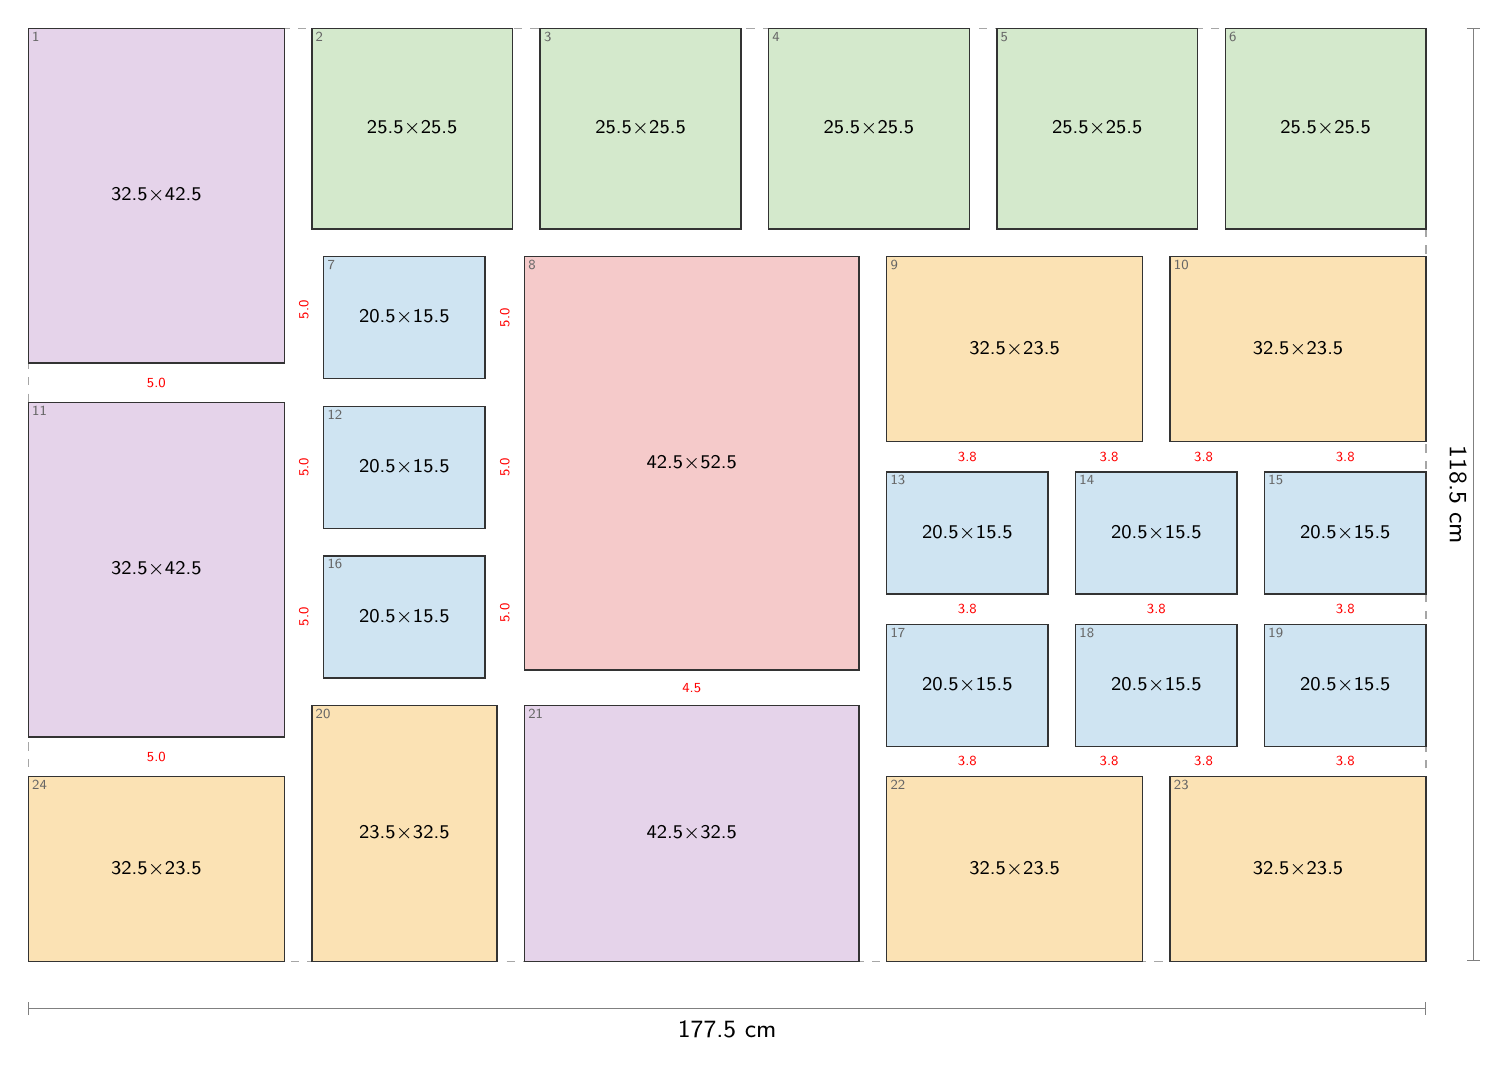
\begin{tikzpicture}[x=1mm, y=-1mm]
\draw[gray!70, dashed, line width=0.4pt] (0,0) rectangle (177.50,118.50);
\filldraw[fill=ft3, draw=black!80, line width=0.5pt] (0.00,0.00) rectangle (32.50,42.50);
\node[align=center, inner sep=0pt] at (16.25,21.25) {\scriptsize 32.5$\times$42.5};
\node[anchor=north west, inner sep=1.2pt, font=\tiny, text=black!60] at (0.00,0.00) {1};
\filldraw[fill=ft2, draw=black!80, line width=0.5pt] (36.00,0.00) rectangle (61.50,25.50);
\node[align=center, inner sep=0pt] at (48.75,12.75) {\scriptsize 25.5$\times$25.5};
\node[anchor=north west, inner sep=1.2pt, font=\tiny, text=black!60] at (36.00,0.00) {2};
\filldraw[fill=ft2, draw=black!80, line width=0.5pt] (65.00,0.00) rectangle (90.50,25.50);
\node[align=center, inner sep=0pt] at (77.75,12.75) {\scriptsize 25.5$\times$25.5};
\node[anchor=north west, inner sep=1.2pt, font=\tiny, text=black!60] at (65.00,0.00) {3};
\filldraw[fill=ft2, draw=black!80, line width=0.5pt] (94.00,0.00) rectangle (119.50,25.50);
\node[align=center, inner sep=0pt] at (106.75,12.75) {\scriptsize 25.5$\times$25.5};
\node[anchor=north west, inner sep=1.2pt, font=\tiny, text=black!60] at (94.00,0.00) {4};
\filldraw[fill=ft2, draw=black!80, line width=0.5pt] (123.00,0.00) rectangle (148.50,25.50);
\node[align=center, inner sep=0pt] at (135.75,12.75) {\scriptsize 25.5$\times$25.5};
\node[anchor=north west, inner sep=1.2pt, font=\tiny, text=black!60] at (123.00,0.00) {5};
\filldraw[fill=ft2, draw=black!80, line width=0.5pt] (152.00,0.00) rectangle (177.50,25.50);
\node[align=center, inner sep=0pt] at (164.75,12.75) {\scriptsize 25.5$\times$25.5};
\node[anchor=north west, inner sep=1.2pt, font=\tiny, text=black!60] at (152.00,0.00) {6};
\filldraw[fill=ft0, draw=black!80, line width=0.5pt] (37.50,29.00) rectangle (58.00,44.50);
\node[align=center, inner sep=0pt] at (47.75,36.75) {\scriptsize 20.5$\times$15.5};
\node[anchor=north west, inner sep=1.2pt, font=\tiny, text=black!60] at (37.50,29.00) {7};
\filldraw[fill=ft4, draw=black!80, line width=0.5pt] (63.00,29.00) rectangle (105.50,81.50);
\node[align=center, inner sep=0pt] at (84.25,55.25) {\scriptsize 42.5$\times$52.5};
\node[anchor=north west, inner sep=1.2pt, font=\tiny, text=black!60] at (63.00,29.00) {8};
\filldraw[fill=ft1, draw=black!80, line width=0.5pt] (109.00,29.00) rectangle (141.50,52.50);
\node[align=center, inner sep=0pt] at (125.25,40.75) {\scriptsize 32.5$\times$23.5};
\node[anchor=north west, inner sep=1.2pt, font=\tiny, text=black!60] at (109.00,29.00) {9};
\filldraw[fill=ft1, draw=black!80, line width=0.5pt] (145.00,29.00) rectangle (177.50,52.50);
\node[align=center, inner sep=0pt] at (161.25,40.75) {\scriptsize 32.5$\times$23.5};
\node[anchor=north west, inner sep=1.2pt, font=\tiny, text=black!60] at (145.00,29.00) {10};
\filldraw[fill=ft3, draw=black!80, line width=0.5pt] (0.00,47.50) rectangle (32.50,90.00);
\node[align=center, inner sep=0pt] at (16.25,68.75) {\scriptsize 32.5$\times$42.5};
\node[anchor=north west, inner sep=1.2pt, font=\tiny, text=black!60] at (0.00,47.50) {11};
\filldraw[fill=ft0, draw=black!80, line width=0.5pt] (37.50,48.00) rectangle (58.00,63.50);
\node[align=center, inner sep=0pt] at (47.75,55.75) {\scriptsize 20.5$\times$15.5};
\node[anchor=north west, inner sep=1.2pt, font=\tiny, text=black!60] at (37.50,48.00) {12};
\filldraw[fill=ft0, draw=black!80, line width=0.5pt] (109.00,56.33) rectangle (129.50,71.83);
\node[align=center, inner sep=0pt] at (119.25,64.08) {\scriptsize 20.5$\times$15.5};
\node[anchor=north west, inner sep=1.2pt, font=\tiny, text=black!60] at (109.00,56.33) {13};
\filldraw[fill=ft0, draw=black!80, line width=0.5pt] (133.00,56.33) rectangle (153.50,71.83);
\node[align=center, inner sep=0pt] at (143.25,64.08) {\scriptsize 20.5$\times$15.5};
\node[anchor=north west, inner sep=1.2pt, font=\tiny, text=black!60] at (133.00,56.33) {14};
\filldraw[fill=ft0, draw=black!80, line width=0.5pt] (157.00,56.33) rectangle (177.50,71.83);
\node[align=center, inner sep=0pt] at (167.25,64.08) {\scriptsize 20.5$\times$15.5};
\node[anchor=north west, inner sep=1.2pt, font=\tiny, text=black!60] at (157.00,56.33) {15};
\filldraw[fill=ft0, draw=black!80, line width=0.5pt] (37.50,67.00) rectangle (58.00,82.50);
\node[align=center, inner sep=0pt] at (47.75,74.75) {\scriptsize 20.5$\times$15.5};
\node[anchor=north west, inner sep=1.2pt, font=\tiny, text=black!60] at (37.50,67.00) {16};
\filldraw[fill=ft0, draw=black!80, line width=0.5pt] (109.00,75.67) rectangle (129.50,91.17);
\node[align=center, inner sep=0pt] at (119.25,83.42) {\scriptsize 20.5$\times$15.5};
\node[anchor=north west, inner sep=1.2pt, font=\tiny, text=black!60] at (109.00,75.67) {17};
\filldraw[fill=ft0, draw=black!80, line width=0.5pt] (133.00,75.67) rectangle (153.50,91.17);
\node[align=center, inner sep=0pt] at (143.25,83.42) {\scriptsize 20.5$\times$15.5};
\node[anchor=north west, inner sep=1.2pt, font=\tiny, text=black!60] at (133.00,75.67) {18};
\filldraw[fill=ft0, draw=black!80, line width=0.5pt] (157.00,75.67) rectangle (177.50,91.17);
\node[align=center, inner sep=0pt] at (167.25,83.42) {\scriptsize 20.5$\times$15.5};
\node[anchor=north west, inner sep=1.2pt, font=\tiny, text=black!60] at (157.00,75.67) {19};
\filldraw[fill=ft1, draw=black!80, line width=0.5pt] (36.00,86.00) rectangle (59.50,118.50);
\node[align=center, inner sep=0pt] at (47.75,102.25) {\scriptsize 23.5$\times$32.5};
\node[anchor=north west, inner sep=1.2pt, font=\tiny, text=black!60] at (36.00,86.00) {20};
\filldraw[fill=ft3, draw=black!80, line width=0.5pt] (63.00,86.00) rectangle (105.50,118.50);
\node[align=center, inner sep=0pt] at (84.25,102.25) {\scriptsize 42.5$\times$32.5};
\node[anchor=north west, inner sep=1.2pt, font=\tiny, text=black!60] at (63.00,86.00) {21};
\filldraw[fill=ft1, draw=black!80, line width=0.5pt] (109.00,95.00) rectangle (141.50,118.50);
\node[align=center, inner sep=0pt] at (125.25,106.75) {\scriptsize 32.5$\times$23.5};
\node[anchor=north west, inner sep=1.2pt, font=\tiny, text=black!60] at (109.00,95.00) {22};
\filldraw[fill=ft1, draw=black!80, line width=0.5pt] (145.00,95.00) rectangle (177.50,118.50);
\node[align=center, inner sep=0pt] at (161.25,106.75) {\scriptsize 32.5$\times$23.5};
\node[anchor=north west, inner sep=1.2pt, font=\tiny, text=black!60] at (145.00,95.00) {23};
\filldraw[fill=ft1, draw=black!80, line width=0.5pt] (0.00,95.00) rectangle (32.50,118.50);
\node[align=center, inner sep=0pt] at (16.25,106.75) {\scriptsize 32.5$\times$23.5};
\node[anchor=north west, inner sep=1.2pt, font=\tiny, text=black!60] at (0.00,95.00) {24};
\node[font=\tiny, text=red, fill=white, inner sep=0.3pt, rotate=90] at (35.00,35.75) {5.0};
\node[font=\tiny, text=red, fill=white, inner sep=0.3pt] at (16.25,45.00) {5.0};
\node[font=\tiny, text=red, fill=white, inner sep=0.3pt, rotate=90] at (60.50,36.75) {5.0};
\node[font=\tiny, text=red, fill=white, inner sep=0.3pt] at (84.25,83.75) {4.5};
\node[font=\tiny, text=red, fill=white, inner sep=0.3pt] at (119.25,54.42) {3.8};
\node[font=\tiny, text=red, fill=white, inner sep=0.3pt] at (137.25,54.42) {3.8};
\node[font=\tiny, text=red, fill=white, inner sep=0.3pt] at (149.25,54.42) {3.8};
\node[font=\tiny, text=red, fill=white, inner sep=0.3pt] at (167.25,54.42) {3.8};
\node[font=\tiny, text=red, fill=white, inner sep=0.3pt, rotate=90] at (35.00,55.75) {5.0};
\node[font=\tiny, text=red, fill=white, inner sep=0.3pt, rotate=90] at (35.00,74.75) {5.0};
\node[font=\tiny, text=red, fill=white, inner sep=0.3pt] at (16.25,92.50) {5.0};
\node[font=\tiny, text=red, fill=white, inner sep=0.3pt, rotate=90] at (60.50,55.75) {5.0};
\node[font=\tiny, text=red, fill=white, inner sep=0.3pt] at (119.25,73.75) {3.8};
\node[font=\tiny, text=red, fill=white, inner sep=0.3pt] at (143.25,73.75) {3.8};
\node[font=\tiny, text=red, fill=white, inner sep=0.3pt] at (167.25,73.75) {3.8};
\node[font=\tiny, text=red, fill=white, inner sep=0.3pt, rotate=90] at (60.50,74.25) {5.0};
\node[font=\tiny, text=red, fill=white, inner sep=0.3pt] at (119.25,93.08) {3.8};
\node[font=\tiny, text=red, fill=white, inner sep=0.3pt] at (137.25,93.08) {3.8};
\node[font=\tiny, text=red, fill=white, inner sep=0.3pt] at (149.25,93.08) {3.8};
\node[font=\tiny, text=red, fill=white, inner sep=0.3pt] at (167.25,93.08) {3.8};
\draw[Bar-Bar, gray] (0,124.50) -- (177.50,124.50) node[midway, below=1pt, font=\small, text=black] {177.5 cm};
\draw[Bar-Bar, gray] (183.50,0) -- (183.50,118.50) node[midway, right=1pt, font=\small, text=black, rotate=-90, anchor=north] {118.5 cm};
\end{tikzpicture}\\[4pt]
{\scriptsize Scale 1:10 (1 mm = 1 cm). Red numbers mark gaps that deviate from the nominal gap by more than 0.25 cm. Small grey numbers index the coordinate table.}
\end{minipage}\hfill
\begin{minipage}[t]{0.25\textwidth}\vspace{0pt}
\small
\begin{tabular}{@{}l l@{}}
\toprule
Outer size & 177.5 $\times$ 118.5 cm \\
Nominal gap & 3.5 cm \\
Actual gaps & 3.5 -- 5.0 cm \\
Max.\ deviation & 1.5 cm \\
Mean deviation & 0.35 cm \\
Border notches & left 10 cm \\
Corners filled & 4 / 4 \\
Frames used & 24 of 28 \\
\bottomrule
\end{tabular}

\vspace{8pt}
\scriptsize
\begin{tabular}{@{}c l l r r@{}}
\toprule
 & outer w $\times$ h (cm) & & used & have \\
\midrule
\tikz[baseline=-0.6ex]\fill[ft0,draw=black!60] (0,0) rectangle (1.2ex,1.2ex); & 20.5$\times$15.5 & L & 9 & 9 \\
\tikz[baseline=-0.6ex]\fill[ft0,draw=black!60] (0,0) rectangle (1.2ex,1.2ex); & 15.5$\times$20.5 & P & 0 & 2 \\
\tikz[baseline=-0.6ex]\fill[ft3,draw=black!60] (0,0) rectangle (1.2ex,1.2ex); & 32.5$\times$42.5 & P & 2 & 2 \\
\tikz[baseline=-0.6ex]\fill[ft3,draw=black!60] (0,0) rectangle (1.2ex,1.2ex); & 42.5$\times$32.5 & L & 1 & 1 \\
\tikz[baseline=-0.6ex]\fill[ft1,draw=black!60] (0,0) rectangle (1.2ex,1.2ex); & 32.5$\times$23.5 & L & 5 & 5 \\
\tikz[baseline=-0.6ex]\fill[ft1,draw=black!60] (0,0) rectangle (1.2ex,1.2ex); & 23.5$\times$32.5 & P & 1 & 1 \\
\tikz[baseline=-0.6ex]\fill[ft2,draw=black!60] (0,0) rectangle (1.2ex,1.2ex); & 25.5$\times$25.5 &  & 5 & 5 \\
\tikz[baseline=-0.6ex]\fill[ft4,draw=black!60] (0,0) rectangle (1.2ex,1.2ex); & 42.5$\times$52.5 & P & 1 & 1 \\
\tikz[baseline=-0.6ex]\fill[ft4,draw=black!60] (0,0) rectangle (1.2ex,1.2ex); & 52.5$\times$42.5 & L & 0 & 2 \\
\bottomrule
\end{tabular}

\vspace{8pt}
{\bfseries Positions} (top-left corner, cm)\\[2pt]
\tiny
\begin{tabular}{@{}r l r r@{}}
\toprule
\# & frame w $\times$ h & x & y \\
\midrule
1 & 32.5 $\times$ 42.5 & 0.0 & 0.0 \\
2 & 25.5 $\times$ 25.5 & 36.0 & 0.0 \\
3 & 25.5 $\times$ 25.5 & 65.0 & 0.0 \\
4 & 25.5 $\times$ 25.5 & 94.0 & 0.0 \\
5 & 25.5 $\times$ 25.5 & 123.0 & 0.0 \\
6 & 25.5 $\times$ 25.5 & 152.0 & 0.0 \\
7 & 20.5 $\times$ 15.5 & 37.5 & 29.0 \\
8 & 42.5 $\times$ 52.5 & 63.0 & 29.0 \\
9 & 32.5 $\times$ 23.5 & 109.0 & 29.0 \\
10 & 32.5 $\times$ 23.5 & 145.0 & 29.0 \\
11 & 32.5 $\times$ 42.5 & 0.0 & 47.5 \\
12 & 20.5 $\times$ 15.5 & 37.5 & 48.0 \\
13 & 20.5 $\times$ 15.5 & 109.0 & 56.3 \\
14 & 20.5 $\times$ 15.5 & 133.0 & 56.3 \\
15 & 20.5 $\times$ 15.5 & 157.0 & 56.3 \\
16 & 20.5 $\times$ 15.5 & 37.5 & 67.0 \\
17 & 20.5 $\times$ 15.5 & 109.0 & 75.7 \\
18 & 20.5 $\times$ 15.5 & 133.0 & 75.7 \\
19 & 20.5 $\times$ 15.5 & 157.0 & 75.7 \\
20 & 23.5 $\times$ 32.5 & 36.0 & 86.0 \\
21 & 42.5 $\times$ 32.5 & 63.0 & 86.0 \\
22 & 32.5 $\times$ 23.5 & 109.0 & 95.0 \\
23 & 32.5 $\times$ 23.5 & 145.0 & 95.0 \\
24 & 32.5 $\times$ 23.5 & 0.0 & 95.0 \\
\bottomrule
\end{tabular}
\end{minipage}
\clearpage

\begin{minipage}[t]{0.74\textwidth}\vspace{0pt}
{\LARGE\bfseries Layout 16}\hspace{1.5em}{\large 172.5 $\times$ 116.5 cm \quad gap 2.5 cm \quad 24 frames}\\[8pt]
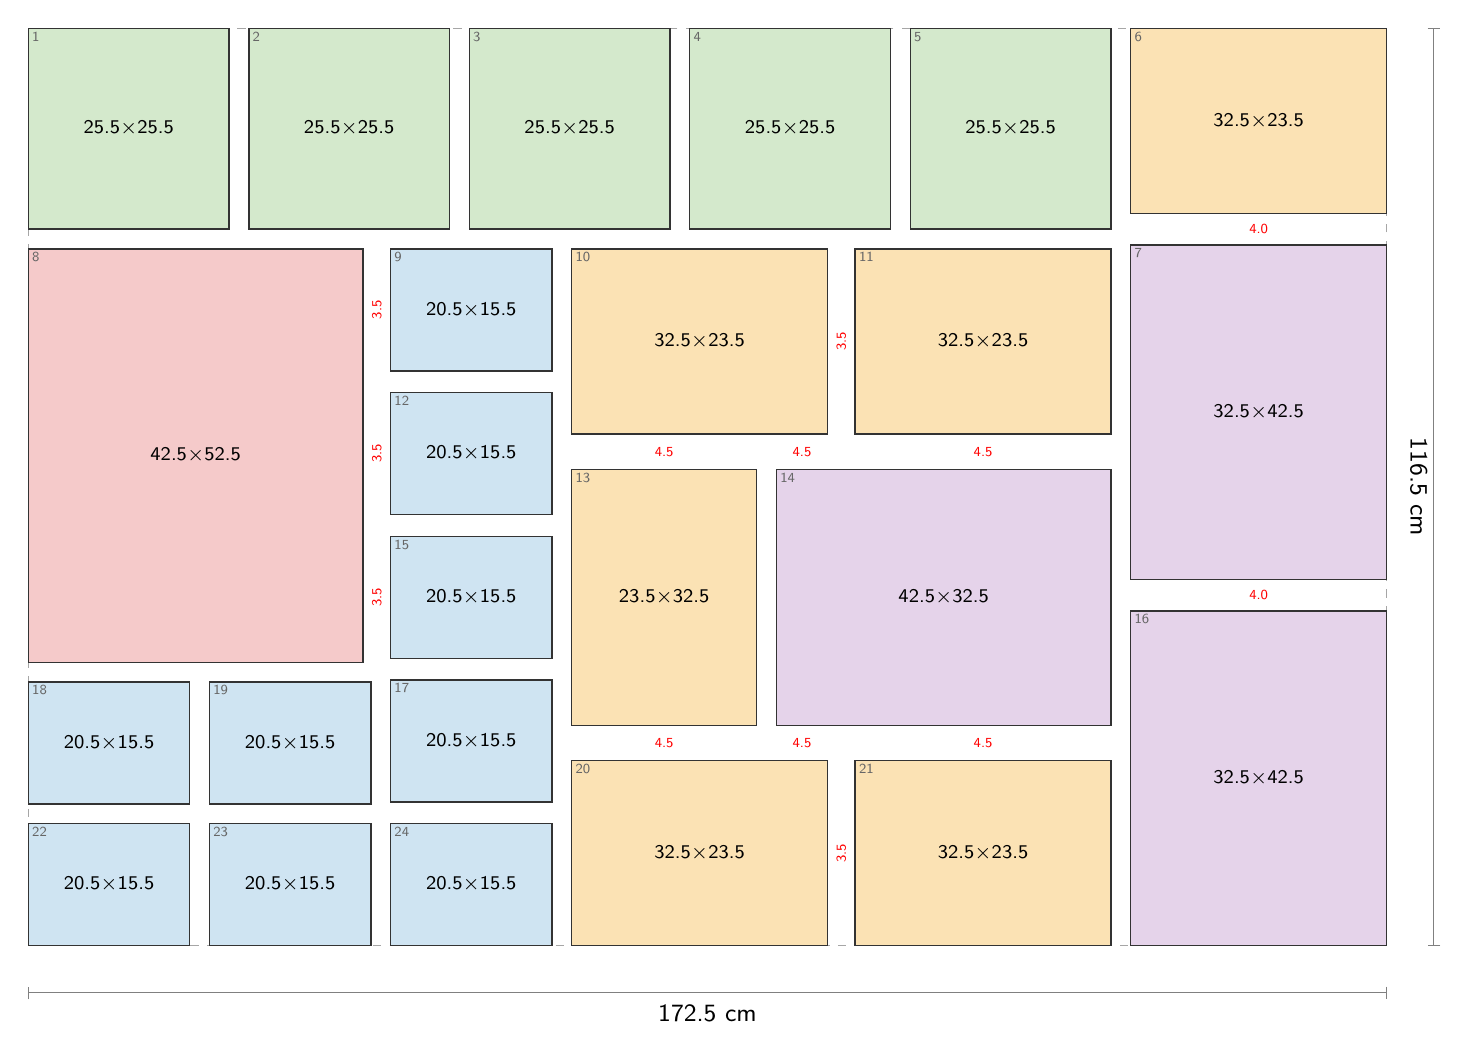
\begin{tikzpicture}[x=1mm, y=-1mm]
\draw[gray!70, dashed, line width=0.4pt] (0,0) rectangle (172.50,116.50);
\filldraw[fill=ft2, draw=black!80, line width=0.5pt] (0.00,0.00) rectangle (25.50,25.50);
\node[align=center, inner sep=0pt] at (12.75,12.75) {\scriptsize 25.5$\times$25.5};
\node[anchor=north west, inner sep=1.2pt, font=\tiny, text=black!60] at (0.00,0.00) {1};
\filldraw[fill=ft2, draw=black!80, line width=0.5pt] (28.00,0.00) rectangle (53.50,25.50);
\node[align=center, inner sep=0pt] at (40.75,12.75) {\scriptsize 25.5$\times$25.5};
\node[anchor=north west, inner sep=1.2pt, font=\tiny, text=black!60] at (28.00,0.00) {2};
\filldraw[fill=ft2, draw=black!80, line width=0.5pt] (56.00,0.00) rectangle (81.50,25.50);
\node[align=center, inner sep=0pt] at (68.75,12.75) {\scriptsize 25.5$\times$25.5};
\node[anchor=north west, inner sep=1.2pt, font=\tiny, text=black!60] at (56.00,0.00) {3};
\filldraw[fill=ft2, draw=black!80, line width=0.5pt] (84.00,0.00) rectangle (109.50,25.50);
\node[align=center, inner sep=0pt] at (96.75,12.75) {\scriptsize 25.5$\times$25.5};
\node[anchor=north west, inner sep=1.2pt, font=\tiny, text=black!60] at (84.00,0.00) {4};
\filldraw[fill=ft2, draw=black!80, line width=0.5pt] (112.00,0.00) rectangle (137.50,25.50);
\node[align=center, inner sep=0pt] at (124.75,12.75) {\scriptsize 25.5$\times$25.5};
\node[anchor=north west, inner sep=1.2pt, font=\tiny, text=black!60] at (112.00,0.00) {5};
\filldraw[fill=ft1, draw=black!80, line width=0.5pt] (140.00,0.00) rectangle (172.50,23.50);
\node[align=center, inner sep=0pt] at (156.25,11.75) {\scriptsize 32.5$\times$23.5};
\node[anchor=north west, inner sep=1.2pt, font=\tiny, text=black!60] at (140.00,0.00) {6};
\filldraw[fill=ft3, draw=black!80, line width=0.5pt] (140.00,27.50) rectangle (172.50,70.00);
\node[align=center, inner sep=0pt] at (156.25,48.75) {\scriptsize 32.5$\times$42.5};
\node[anchor=north west, inner sep=1.2pt, font=\tiny, text=black!60] at (140.00,27.50) {7};
\filldraw[fill=ft4, draw=black!80, line width=0.5pt] (0.00,28.00) rectangle (42.50,80.50);
\node[align=center, inner sep=0pt] at (21.25,54.25) {\scriptsize 42.5$\times$52.5};
\node[anchor=north west, inner sep=1.2pt, font=\tiny, text=black!60] at (0.00,28.00) {8};
\filldraw[fill=ft0, draw=black!80, line width=0.5pt] (46.00,28.00) rectangle (66.50,43.50);
\node[align=center, inner sep=0pt] at (56.25,35.75) {\scriptsize 20.5$\times$15.5};
\node[anchor=north west, inner sep=1.2pt, font=\tiny, text=black!60] at (46.00,28.00) {9};
\filldraw[fill=ft1, draw=black!80, line width=0.5pt] (69.00,28.00) rectangle (101.50,51.50);
\node[align=center, inner sep=0pt] at (85.25,39.75) {\scriptsize 32.5$\times$23.5};
\node[anchor=north west, inner sep=1.2pt, font=\tiny, text=black!60] at (69.00,28.00) {10};
\filldraw[fill=ft1, draw=black!80, line width=0.5pt] (105.00,28.00) rectangle (137.50,51.50);
\node[align=center, inner sep=0pt] at (121.25,39.75) {\scriptsize 32.5$\times$23.5};
\node[anchor=north west, inner sep=1.2pt, font=\tiny, text=black!60] at (105.00,28.00) {11};
\filldraw[fill=ft0, draw=black!80, line width=0.5pt] (46.00,46.25) rectangle (66.50,61.75);
\node[align=center, inner sep=0pt] at (56.25,54.00) {\scriptsize 20.5$\times$15.5};
\node[anchor=north west, inner sep=1.2pt, font=\tiny, text=black!60] at (46.00,46.25) {12};
\filldraw[fill=ft1, draw=black!80, line width=0.5pt] (69.00,56.00) rectangle (92.50,88.50);
\node[align=center, inner sep=0pt] at (80.75,72.25) {\scriptsize 23.5$\times$32.5};
\node[anchor=north west, inner sep=1.2pt, font=\tiny, text=black!60] at (69.00,56.00) {13};
\filldraw[fill=ft3, draw=black!80, line width=0.5pt] (95.00,56.00) rectangle (137.50,88.50);
\node[align=center, inner sep=0pt] at (116.25,72.25) {\scriptsize 42.5$\times$32.5};
\node[anchor=north west, inner sep=1.2pt, font=\tiny, text=black!60] at (95.00,56.00) {14};
\filldraw[fill=ft0, draw=black!80, line width=0.5pt] (46.00,64.50) rectangle (66.50,80.00);
\node[align=center, inner sep=0pt] at (56.25,72.25) {\scriptsize 20.5$\times$15.5};
\node[anchor=north west, inner sep=1.2pt, font=\tiny, text=black!60] at (46.00,64.50) {15};
\filldraw[fill=ft3, draw=black!80, line width=0.5pt] (140.00,74.00) rectangle (172.50,116.50);
\node[align=center, inner sep=0pt] at (156.25,95.25) {\scriptsize 32.5$\times$42.5};
\node[anchor=north west, inner sep=1.2pt, font=\tiny, text=black!60] at (140.00,74.00) {16};
\filldraw[fill=ft0, draw=black!80, line width=0.5pt] (46.00,82.75) rectangle (66.50,98.25);
\node[align=center, inner sep=0pt] at (56.25,90.50) {\scriptsize 20.5$\times$15.5};
\node[anchor=north west, inner sep=1.2pt, font=\tiny, text=black!60] at (46.00,82.75) {17};
\filldraw[fill=ft0, draw=black!80, line width=0.5pt] (0.00,83.00) rectangle (20.50,98.50);
\node[align=center, inner sep=0pt] at (10.25,90.75) {\scriptsize 20.5$\times$15.5};
\node[anchor=north west, inner sep=1.2pt, font=\tiny, text=black!60] at (0.00,83.00) {18};
\filldraw[fill=ft0, draw=black!80, line width=0.5pt] (23.00,83.00) rectangle (43.50,98.50);
\node[align=center, inner sep=0pt] at (33.25,90.75) {\scriptsize 20.5$\times$15.5};
\node[anchor=north west, inner sep=1.2pt, font=\tiny, text=black!60] at (23.00,83.00) {19};
\filldraw[fill=ft1, draw=black!80, line width=0.5pt] (69.00,93.00) rectangle (101.50,116.50);
\node[align=center, inner sep=0pt] at (85.25,104.75) {\scriptsize 32.5$\times$23.5};
\node[anchor=north west, inner sep=1.2pt, font=\tiny, text=black!60] at (69.00,93.00) {20};
\filldraw[fill=ft1, draw=black!80, line width=0.5pt] (105.00,93.00) rectangle (137.50,116.50);
\node[align=center, inner sep=0pt] at (121.25,104.75) {\scriptsize 32.5$\times$23.5};
\node[anchor=north west, inner sep=1.2pt, font=\tiny, text=black!60] at (105.00,93.00) {21};
\filldraw[fill=ft0, draw=black!80, line width=0.5pt] (0.00,101.00) rectangle (20.50,116.50);
\node[align=center, inner sep=0pt] at (10.25,108.75) {\scriptsize 20.5$\times$15.5};
\node[anchor=north west, inner sep=1.2pt, font=\tiny, text=black!60] at (0.00,101.00) {22};
\filldraw[fill=ft0, draw=black!80, line width=0.5pt] (23.00,101.00) rectangle (43.50,116.50);
\node[align=center, inner sep=0pt] at (33.25,108.75) {\scriptsize 20.5$\times$15.5};
\node[anchor=north west, inner sep=1.2pt, font=\tiny, text=black!60] at (23.00,101.00) {23};
\filldraw[fill=ft0, draw=black!80, line width=0.5pt] (46.00,101.00) rectangle (66.50,116.50);
\node[align=center, inner sep=0pt] at (56.25,108.75) {\scriptsize 20.5$\times$15.5};
\node[anchor=north west, inner sep=1.2pt, font=\tiny, text=black!60] at (46.00,101.00) {24};
\node[font=\tiny, text=red, fill=white, inner sep=0.3pt] at (156.25,25.50) {4.0};
\node[font=\tiny, text=red, fill=white, inner sep=0.3pt] at (156.25,72.00) {4.0};
\node[font=\tiny, text=red, fill=white, inner sep=0.3pt, rotate=90] at (44.25,35.75) {3.5};
\node[font=\tiny, text=red, fill=white, inner sep=0.3pt, rotate=90] at (44.25,54.00) {3.5};
\node[font=\tiny, text=red, fill=white, inner sep=0.3pt, rotate=90] at (44.25,72.25) {3.5};
\node[font=\tiny, text=red, fill=white, inner sep=0.3pt, rotate=90] at (103.25,39.75) {3.5};
\node[font=\tiny, text=red, fill=white, inner sep=0.3pt] at (80.75,53.75) {4.5};
\node[font=\tiny, text=red, fill=white, inner sep=0.3pt] at (98.25,53.75) {4.5};
\node[font=\tiny, text=red, fill=white, inner sep=0.3pt] at (121.25,53.75) {4.5};
\node[font=\tiny, text=red, fill=white, inner sep=0.3pt] at (80.75,90.75) {4.5};
\node[font=\tiny, text=red, fill=white, inner sep=0.3pt] at (98.25,90.75) {4.5};
\node[font=\tiny, text=red, fill=white, inner sep=0.3pt] at (121.25,90.75) {4.5};
\node[font=\tiny, text=red, fill=white, inner sep=0.3pt, rotate=90] at (103.25,104.75) {3.5};
\draw[Bar-Bar, gray] (0,122.50) -- (172.50,122.50) node[midway, below=1pt, font=\small, text=black] {172.5 cm};
\draw[Bar-Bar, gray] (178.50,0) -- (178.50,116.50) node[midway, right=1pt, font=\small, text=black, rotate=-90, anchor=north] {116.5 cm};
\end{tikzpicture}\\[4pt]
{\scriptsize Scale 1:10 (1 mm = 1 cm). Red numbers mark gaps that deviate from the nominal gap by more than 0.25 cm. Small grey numbers index the coordinate table.}
\end{minipage}\hfill
\begin{minipage}[t]{0.25\textwidth}\vspace{0pt}
\small
\begin{tabular}{@{}l l@{}}
\toprule
Outer size & 172.5 $\times$ 116.5 cm \\
Nominal gap & 2.5 cm \\
Actual gaps & 2.5 -- 4.5 cm \\
Max.\ deviation & 2.0 cm \\
Mean deviation & 0.43 cm \\
Border notches & right 8 cm \\
Corners filled & 4 / 4 \\
Frames used & 24 of 28 \\
\bottomrule
\end{tabular}

\vspace{8pt}
\scriptsize
\begin{tabular}{@{}c l l r r@{}}
\toprule
 & outer w $\times$ h (cm) & & used & have \\
\midrule
\tikz[baseline=-0.6ex]\fill[ft0,draw=black!60] (0,0) rectangle (1.2ex,1.2ex); & 20.5$\times$15.5 & L & 9 & 9 \\
\tikz[baseline=-0.6ex]\fill[ft0,draw=black!60] (0,0) rectangle (1.2ex,1.2ex); & 15.5$\times$20.5 & P & 0 & 2 \\
\tikz[baseline=-0.6ex]\fill[ft3,draw=black!60] (0,0) rectangle (1.2ex,1.2ex); & 32.5$\times$42.5 & P & 2 & 2 \\
\tikz[baseline=-0.6ex]\fill[ft3,draw=black!60] (0,0) rectangle (1.2ex,1.2ex); & 42.5$\times$32.5 & L & 1 & 1 \\
\tikz[baseline=-0.6ex]\fill[ft1,draw=black!60] (0,0) rectangle (1.2ex,1.2ex); & 32.5$\times$23.5 & L & 5 & 5 \\
\tikz[baseline=-0.6ex]\fill[ft1,draw=black!60] (0,0) rectangle (1.2ex,1.2ex); & 23.5$\times$32.5 & P & 1 & 1 \\
\tikz[baseline=-0.6ex]\fill[ft2,draw=black!60] (0,0) rectangle (1.2ex,1.2ex); & 25.5$\times$25.5 &  & 5 & 5 \\
\tikz[baseline=-0.6ex]\fill[ft4,draw=black!60] (0,0) rectangle (1.2ex,1.2ex); & 42.5$\times$52.5 & P & 1 & 1 \\
\tikz[baseline=-0.6ex]\fill[ft4,draw=black!60] (0,0) rectangle (1.2ex,1.2ex); & 52.5$\times$42.5 & L & 0 & 2 \\
\bottomrule
\end{tabular}

\vspace{8pt}
{\bfseries Positions} (top-left corner, cm)\\[2pt]
\tiny
\begin{tabular}{@{}r l r r@{}}
\toprule
\# & frame w $\times$ h & x & y \\
\midrule
1 & 25.5 $\times$ 25.5 & 0.0 & 0.0 \\
2 & 25.5 $\times$ 25.5 & 28.0 & 0.0 \\
3 & 25.5 $\times$ 25.5 & 56.0 & 0.0 \\
4 & 25.5 $\times$ 25.5 & 84.0 & 0.0 \\
5 & 25.5 $\times$ 25.5 & 112.0 & 0.0 \\
6 & 32.5 $\times$ 23.5 & 140.0 & 0.0 \\
7 & 32.5 $\times$ 42.5 & 140.0 & 27.5 \\
8 & 42.5 $\times$ 52.5 & 0.0 & 28.0 \\
9 & 20.5 $\times$ 15.5 & 46.0 & 28.0 \\
10 & 32.5 $\times$ 23.5 & 69.0 & 28.0 \\
11 & 32.5 $\times$ 23.5 & 105.0 & 28.0 \\
12 & 20.5 $\times$ 15.5 & 46.0 & 46.2 \\
13 & 23.5 $\times$ 32.5 & 69.0 & 56.0 \\
14 & 42.5 $\times$ 32.5 & 95.0 & 56.0 \\
15 & 20.5 $\times$ 15.5 & 46.0 & 64.5 \\
16 & 32.5 $\times$ 42.5 & 140.0 & 74.0 \\
17 & 20.5 $\times$ 15.5 & 46.0 & 82.8 \\
18 & 20.5 $\times$ 15.5 & 0.0 & 83.0 \\
19 & 20.5 $\times$ 15.5 & 23.0 & 83.0 \\
20 & 32.5 $\times$ 23.5 & 69.0 & 93.0 \\
21 & 32.5 $\times$ 23.5 & 105.0 & 93.0 \\
22 & 20.5 $\times$ 15.5 & 0.0 & 101.0 \\
23 & 20.5 $\times$ 15.5 & 23.0 & 101.0 \\
24 & 20.5 $\times$ 15.5 & 46.0 & 101.0 \\
\bottomrule
\end{tabular}
\end{minipage}
\clearpage

\end{document}
